%!TEX TS-program = xelatex
%!TEX encoding = UTF-8 Unicode

\documentclass[
	%12pt,
	%b5paper,
	twoside,
	openright,
]{book}

\usepackage[cam,a4,center]{crop}

\usepackage{imakeidx}
\usepackage[T1]{fontenc}

\usepackage[
  paperheight=26cm,
	paperwidth=13cm,
	top=1.23in,
	bottom=1.23in,
	left=1cm,
	right=1cm,
	%margin=0.707in,
	% pass,
	showframe,
	bindingoffset=6mm,
	verbose,
	heightrounded
]{geometry}

\usepackage[parfill]{parskip}
\usepackage{graphicx}
\usepackage{amssymb}
\usepackage{wrapfig}
\usepackage{float}
\usepackage{mdframed}

\usepackage{paralist}
\usepackage{array}
\usepackage{longtable}
\usepackage{multirow}

\usepackage{url}
\usepackage[colorlinks]{hyperref}
\hypersetup{citecolor=black}
\hypersetup{linkcolor=black}
\hypersetup{urlcolor=black}
\usepackage{cleveref}

\usepackage{microtype} % Improves spacing
\usepackage{multicol}
\usepackage{pdfpages}

\usepackage{tikz}
\usetikzlibrary{shapes.geometric}
\usetikzlibrary{matrix}
\usetikzlibrary{snakes}

\usepackage{color}
\usepackage{lipsum}

\usepackage[
	framed,
	numbered
]{sclang-prettifier}

\makeindex[title=Indice dei nomi]

\graphicspath{{images/}}

\usepackage[
	autostyle,
	italian=guillemets,
	% altre opzioni
	]{csquotes}

\newmdenv[
	topline=false,
	bottomline=false,
	skipabove=\topsep,
	skipbelow=\topsep
	]{siderules}

\usepackage[
	% altre opzioni,
	style=authoryear,
	%backend=biber
]{biblatex}

\addbibresource{musebib/nono-luigi.bib}
\addbibresource{musebib/novecento.bib}


%-------------------------------------------------------------
%----------------------------------------------------- FONTS -
%-------------------------------------------------------------

\linespread{1.04}

\usepackage{etoolbox}

\usepackage{fontspec,
			xltxtra,
			xunicode
			}

\defaultfontfeatures{Mapping=tex-text}

\setromanfont[
	Mapping=tex-text
	]{Alegreya}

\setsansfont[
	Scale=MatchLowercase,
	Mapping=tex-text,
	% LetterSpace=3.0,
	% Scale=0.707,
	]{Fira Sans}

\setmonofont[]{Fira Mono}

\newfontfamily{\scaps}{Alegreya SC}

\newfontfamily\quotefont[
	Scale=MatchLowercase,
	Mapping=tex-text,
	LetterSpace=3.0,
	%Scale=1.123,
	]{Fira Sans}
\AtBeginEnvironment{quote}{\quotefont\small}

\usepackage[
	english,
	italian,
	]{babel}

\usepackage{lilyglyphs}

\usepackage[
	hang,
	small,
	labelfont=bf,
	up,
	textfont=it,
	up
	]{caption}

%-------------------------------------------------------------
%------------------------------------------------ TIPOGRAFIA -
%-------------------------------------------------------------

\setlength{\columnsep}{.4in}

\setcounter{secnumdepth}{3}
\setcounter{tocdepth}{1}

\usepackage{changepage}

%-------------------------------------------------------------
%---------------------------------------------------- HEADER -
%-------------------------------------------------------------

\usepackage{fancyhdr}

\fancypagestyle{plain}{%
\fancyhf{} % clear all header and footer fields
%\fancyhead[CO,CE]{---Draft---}
\fancyfoot[RO,LE]{\fontsize{18pt}{18pt}\selectfont\thepage} % except the center
\renewcommand{\headrulewidth}{0pt}
\renewcommand{\footrulewidth}{0pt}}
\pagestyle{plain}

%-------------------------------------------------------------
%---------------------------------------------- COPERTINA BG -
%-------------------------------------------------------------

\makeatletter
%\frameattext{<backgroundcolor>}{linecolor}{<linewidth>}
\newdimen\extraxsep
\newdimen\extraysep
\extraxsep=20mm
\extraysep=20mm
\newcommand\frameattext[3]{%
  \linethickness{#3}%
  \AddToShipoutPicture*{%
    \AtTextLowerLeft{%text-boder
       \put(\LenToUnit{-,5\extraxsep},\LenToUnit{-0.5\extraysep}){\color{#1}%
             \rule{\dimexpr\textwidth+\extraxsep\relax}{\dimexpr\textheight+\extraysep\relax}}%
       \put(\LenToUnit{-,5\extraxsep},\LenToUnit{-0.5\extraysep}){\color{#2}%
       \framebox(\LenToUnit{\dimexpr\textwidth+\extraxsep\relax},%
                 \LenToUnit{\dimexpr\textheight+\extraysep\relax}){}
       }
    }%
  }%
}
%\frameatpage{<backgroundcolor>}{linecolor}{<linewidth>}
\newcommand\frameatpage[3]{%
  \linethickness{#3}%
  \AddToShipoutPicture*{%
    \AtPageLowerLeft{%page-border
      \put(0,0){\color{#1}\rule{\paperwidth}{\paperheight}}%
      \put(\LenToUnit{\@wholewidth},\LenToUnit{\@wholewidth}){%
       \color{#2}\framebox(\LenToUnit{\dimexpr\paperwidth-2\@wholewidth\relax},%
                  \LenToUnit{\dimexpr\paperheight-2\@wholewidth\relax}){}%
      }%
    }%
  }%
}

\makeatother


%-------------------------------------------------------------
%--------------------------------------------- CHAPTER PHOTO -
%-------------------------------------------------------------

% \makeatletter
% \newcommand\ChapImage{\includepdf[
% 	scale=1.05,
% 	pagecommand={
% 		\begin{tikzpicture}[
% 		remember picture,
% 		overlay
% 		]
% 			\node [xshift=2cm,yshift=1cm] at (current page.south west) {\color{white}{\emph{Roberto \textbf{Masotti}}}};
% 			\end{tikzpicture}}
% 			]{images/masotti/cage.pdf}
% 			}
% \newcommand*\Invcleardoublepage{
% \clearpage\if@twoside
%   \ifodd\c@page \null\newpage\if@twocolumn\null%
%   \newpage\fi\fi\fi
% }
% \renewcommand\chapter{%
%   \if@openright
%     \ifodd\c@page{\Invcleardoublepage}\else{\clearpage}\fi
%     {
%     \pagestyle{empty}
%     \ChapImage
%     \clearpage
%     }
%   \else
%     \clearpage
%   \fi
%   \thispagestyle{\chapterpagestyle}%
%   \global\@topnum\z@
%   \@afterindentfalse
%   \secdef\@chapter\@schapter
% }
% \makeatother

\newcommand{\link}[2]{\href{#1}{{#2}$%
            \blacktriangleright
						\blacktriangleright
						\blacktriangleright%
						$}}

\newcommand{\bianca}{$%
            ~%
            \thispagestyle{empty}%
            \clearpage%
						$}

\newcommand{\entry}[4]{\textbf{#1}\markboth{#1}{#1}\ {(#2)}\ \textit{#3}\ $\bullet$\ {#4}} % Defines the command to print each word on the page, \markboth{}{} prints the first word on the page in the top left header and the last word in the top right

%-------------------------------------------------------------
%-------------------------------------------------- DOCUMENT -
%-------------------------------------------------------------

\begin{document}

%-------------------------------------------------------------
%------------------------------------------------- COPERTINA -
%-------------------------------------------------------------

\AddToShipoutPictureBG*{%
	\put(-60,-10){
	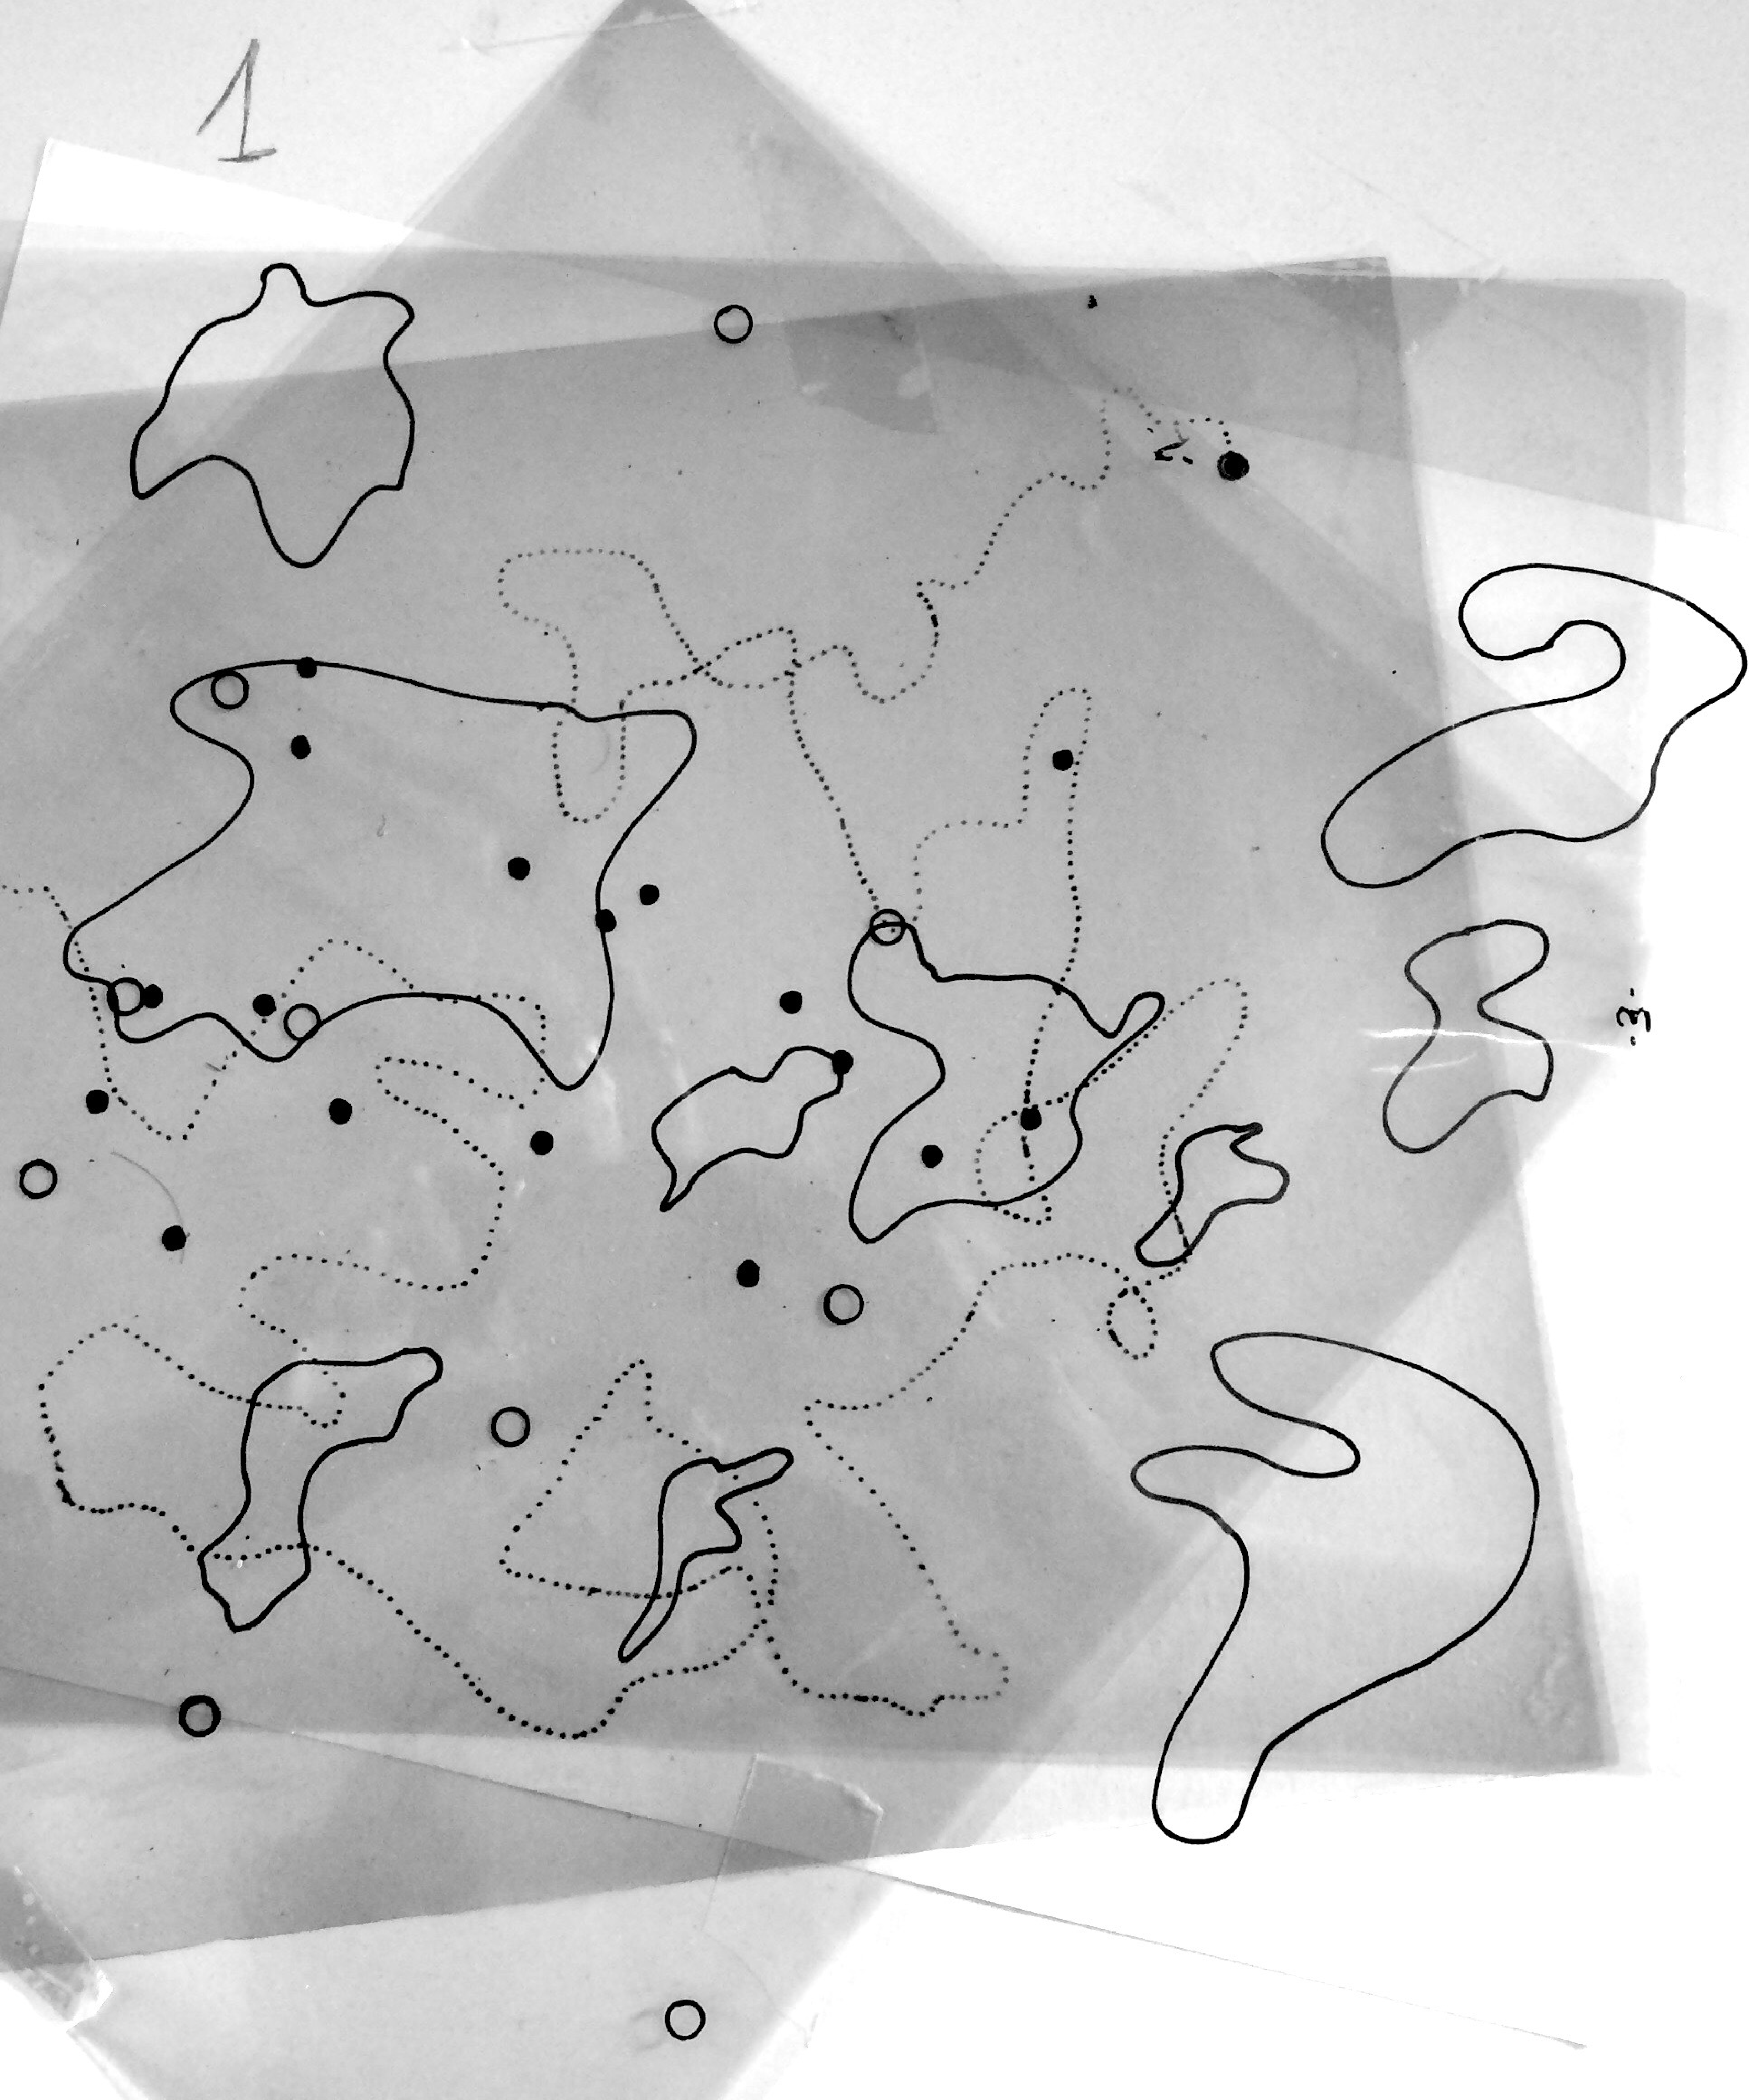
\includegraphics[keepaspectratio,scale=.3123]{bg}}
	}

\frameattext{white}{black}{2pt}

\begin{center}

	~

	\vfill

  \fontsize{19}{19}\selectfont{Giuseppe SILVI}

	\vspace{.23in}

	\noindent\makebox[\linewidth]{\rule{.3\paperwidth}{1pt}}

	\fontsize{51}{51}\selectfont{\emph{l'invito \\ all'ascolto}} \\

	\vfill %\vspace{1in}
	~
	\vfill

	\fontsize{19}{19}\selectfont{Antologia elettroacustica}

	% \bigskip
	%
  % \fontsize{19}{19}\selectfont{
	% 		\emph{COME/01 \\
	% 		Esecuzione ed Interpretazione della \\
	% 		Musica elettroacustica \\
	% 		2016/2019}
	% 		} \\

	\vfill

	\fontsize{13}{13}\selectfont{draft \emph{\# 003}\\ \today}

	\vfill

	~

\end{center}

\thispagestyle{empty}

\clearpage


%!TEX TS-program = xelatex
%!TEX encoding = UTF-8 Unicode
% !TEX root = ../../2017-GS-COME01-INVITO-ASCOLTO.tex

%-------------------------------------------------------------
%-------------------------------------------------- COLOPHON -
%-------------------------------------------------------------

\thispagestyle{empty}

Conservatorio di Musica S. Cecilia di Roma \\
DIPARTIMENTO DI MUSICA ELETTRONICA \\
\emph{Esecuzione ed Interpretazione della Musica Elettronica - COME/01} \\
Triennio Accademico 2016-2019
\vfill

Attribution 4.0 International (CC BY 4.0)

You are free to:
\begin{description}
	\item[Share] - copy and redistribute the material in any medium or format
	\item[Adapt] - remix, transform, and build upon the material for any purpose, even commercially.
\end{description}

Under the following terms:
\begin{description}
	\item[Attribution] You must give appropriate credit, provide a link to the license, and indicate if
	changes were made. You may do so in any reasonable manner, but not in any way that suggests the licensor
	endorses you or your use.
	\item[No additional restrictions] You may not apply legal terms or technological measures that legally
	restrict others from doing anything the license permits.
\end{description}

Notices:\\
You do not have to comply with the license for elements of the material in the public domain or where your
use is permitted by an applicable exception or limitation. No warranties are given. The license may not give
you all of the permissions necessary for your intended use. For example, other rights such as publicity,
privacy, or moral rights may limit how you use the material.

\clearpage


%-------------------------------------------------------------
%---------------------------------------------------- INDICE -
%-------------------------------------------------------------

\tableofcontents
\thispagestyle{empty}

\bianca
\input{includes/capitoli/0002-PREMESSA.tex}

%!TEX TS-program = xelatex
%!TEX encoding = UTF-8 Unicode
% !TEX root = ../../2017-GS-COME01-INVITO-ASCOLTO.tex

%-------------------------------------------------------------
%---------------------------------------------- INTRODUZIONE -
%-------------------------------------------------------------

\chapter*{Introduzione}
\addcontentsline{toc}{chapter}{Introduzione}

Operando la scelta dei brani per il corso di interpretazione ho provato a rispondere ad una domanda piuttosto semplice quanto necessaria: \emph{perché fare repertorio?} Questa domanda, prima di risposte, ha generato una successiva domanda: \emph{cos'è repertorio?} Ed anche rispondendo a queste prime domande ne è emersa una successiva: \emph{qual è il ruolo del repertorio nel fare contemporaneo?} Si ma \emph{cos'è contemporaneo?}.

%Attraverso l'oscuro di questi dubbi ho individuato l'oscuro argomento del mio corso, quindi il focus sul repertorio: l'\emph{ascolto}. \emph{Fare repertorio nell'espressione del suo senso pi\`u completo \`e imparare ad ascoltare.}

Dato che le domande sono strettamente intrecciate tra loro, proverei a dare una prima definizione di uomo contemporaneo con le parole di Agamben\index{Agamben, Giorgio}:

\begin{quote}
	Contemporaneo è colui che riceve in pieno viso il fascio di tenebra che proviene dal suo tempo.
\end{quote}

È una definizione fortemente poetica che pone di nuovo la percezione al centro dell'asse uomo-tenebra.
La contemporaneità è quindi un momento mobile del tempo che identifica la facoltà di osservare l'oscurità del tempo specifico.

L'osservazione può avvenire solo per distanza perché il contemporaneo, affinando la definizione con le parole di Nietzche, è intempestivo, inattuale.

\begin{quote}
	Appartiene veramente al suo tempo, è veramente contemporaneo colui che non coincide perfettamente con esso, non si adegua alle sue pretese ed è perciò, in questo senzo, inattuale; ma proprio per questo scarto e questo anacronismo, egli è capace pi\`u degli altri di percepire ed afferrare il suo tempo.
\end{quote}

La contemporaneità è quindi

\begin{quote}
	quella relazione col tempo che aderisce a esso attraverso una sfasatura e un anacronismo
\end{quote}

che ci permette di valutare, vedere ed analizzare, alla dovuta distanza. Spazio e tempo quindi legati nell'istante percettivo.

Il tempo del nostro repertorio

\begin{quote}
	è la contemporaneità, esso esige di essere contemporaneo dei testi e degli autori che esamina.
\end{quote}

Attraverso l'oscuro di questi dubbi ho individuato l'oscuro argomento del mio corso, quindi il repertorio, l'\emph{ascolto}: \emph{fare repertorio nell'espressione del suo senso pi\`u completo \`e imparare ad ascoltare.}

Crescere in un processo analitico-conoscitivo che amplifichi le capacità percettive, interpretando, nel significato pratico del termine, praticando. In questa direzione ho reso superfluo chiedersi \emph{perché fare repertorio} (per imparare ad ascoltare risponderemmo) ma al suo posto sorge spontaneamente la domanda \emph{come?} \emph{Come si fa repertorio?} Credo si possa fare repertorio solo ricostruendo, assemblando contesti sulle informazioni disponibili, affinch\'e la pratica poggi su una coscienza, ricostruita, che si stratifichi come pietra calcarea nel sapere sociale. Solo in questo senso il repertorio può essere, al pari della scrittura, esercizio, necessità, nutrimento della percezione.

\begin{quote}
	Alla scarsa attenzione alla problematica musicale da parte della riflessione estetica e filosofica in genere, fa riscontro - e alludo qui naturalmente in modo esclusivo alla situazione italiana - nei confronti della questione di una teoria generale della musica, disinteresse che non ha conseguenze solo su maggiori o minori profondità speculative, ma che ha generato una relativa arretratezza nel campo delle indagini pi\`u strettamente analitiche che esigono in via di principio opzioni di ordine teorico e metodico spesso apertamente confinanti nell'ambito delle questioni filosofiche [\ldots] La necessità di un punto di vista di una teoria generale si impone qui con particolare evidenza in stretta connessione con problematiche analitiche specifiche e con la consapevolezza del suo raggio di azione che raggiunge il problema della costruzione di un apparato categoriale capace di offrire strumenti per la comprensione delle strutture musicali di culture non europee, così come quello di un  rinnovamento della presentazione dei \emph{concetti fondamentali} che non può non avere conseguenze importanti nella didattica musicale. \footnote{Giovanni Piana (1991, p. 253, nota 14)}
\end{quote}

È un procedere che stratifica, solidifica conoscenza. Dopo aver studiato, letto ed interpretato \emph{Mantra} non si può tornare ad uno strato inferiore di coscienza, ad uno strato precedente di conoscenza. \emph{Mantra} si presenta come un paradigma del sapere musicale. Allo stesso tempo musicale, Cage, illumina la musica, sorride al senso del fare musica, porta l'idea di interprete ad un livello superiore, di manipolazione dell'idea, ai confini della libertà musicale e sociale, li dove spesso la mancata consapevolezza lascia smarriti e senza anima.


%!TEX TS-program = xelatex
%!TEX encoding = UTF-8 Unicode
% !TEX root = ../../2017-GS-COME01-INVITO-ASCOLTO.tex

%-------------------------------------------------------------
%----------------------------- SUONO. SEGNO. INTERPRETAZIONE -
%-------------------------------------------------------------

\chapter*{Suono. Segno. Interpretazione.}
\addcontentsline{toc}{chapter}{Suono. Segno. Interpretazione.}

	\begin{flushright}
		\textit{Nella nostra anima c'\`e una incrinatura che, se sfiorata, \\
		risuona come un vaso prezioso riemerso dalle profondit\`a della terra} \\
		Wassilly Kandinsky - \emph{Lo Spirituale nell'Arte}
	\end{flushright}

	\begin{flushright}
		\textit{Music of Changes // John ChAnGEs} \\
		Pierre Boulez
	\end{flushright}

	\begin{flushright}
		\textit{Si dice che i compositori abbiano orecchio per la musica e \\
		di solito significa che non sentono nulla che arrivi alle loro orecchie. \\
		Le loro orecchie sono murate dai suoni di loro creazione.} \\
		John Cage - \emph{45' for a Speaker} (1954)
	\end{flushright}

\bigskip

%\begin{multicols}{2}

Le percezioni cambiano con il tempo. Ci sono diversi tempi, anche simultanei, del cambiamento.
Il tempo ciclico della riflessione. È quello breve, del pensiero ricorsivo, che non torna mai su se stesso identico al se stesso precedente.
In questo tempo la percezione stratifica, l'oggetto di senso percepito, osservato, muta, ne evolve il significato.
L'apparente movimento ciclico del pensiero ricorsivo non si muove ad anello, nbensì in una sorta di spirale per cui sì, bidimensionalmente, può apparire un ritornare, ma ad una visione almeno tridimensionale questo appare a forma di spirale.
Quadrimensionalmente questa è una spirale che si muove nel tempo, che quindi accupa uno spazio temporale ampio, del divenire. Due tempi quindi, quello ciclico, ricorsivo, e quello lungo, della mutazione nelle spazio-tempo.

\begin{tikzpicture}[segment amplitude=10pt]
  \draw[snake=coil]                  (0,1) -- (3,1);
  %\draw[snake=coil,segment aspect=0] (0,0) -- (3,0);
\end{tikzpicture}

A queste percezioni che mutano nel tempo e nello spazio siamo abituati a dare nomi. Suono, è un nome.
L'idea di suono è separata dalla cosa che rappresenta.
Potremmo dire che il suo significato è rimasto quasi invariato nel corso dei tempi
In questo gli studi etimologici sono strumenti indispensabili.
Il rapporto sensoriale che identificheremo con le parole cambiano però piuttosto rapidamente.
Con la parola suono definiamo una percezione. Definiamo suono una percezione.
Il suo significato risale a epoche antiche.

Le arti del tempo condividono la stessa struttura percettiva: un testo fissato ed il suo alter ego evento momentaneo.

\begin{quote}
	la scrittura in tutti i campi si costituisce nel momento in cui si può disporre di un sistema di marcatori visivi che assolvono a fruizioni precedentemente affidate alla memoria o ad altri artifici più rudimentali\footnote{borio 9}
\end{quote}

Suono e Segno. I due stati dell'oggettivazione musicale sui quali l'interpretazione, sguardo ad oggettività limitata, vede collegamenti e potenzialità. Suono e gesto viaggiano su un asse temporale diverso da quello della sua rappresentazione. Ma circoscrivere il segno a “semplice” rappresentazione è grossolanamente sbagliato.

Se suono e gesto possiedono un tempo separato da quella della sua rappresentazione (tradizione orale) allora c'è da domandarsi cosa la scrittura abbia aggiunto e se si è verificata una eventuale perdita.

\begin{quote}
	il testo musicale [\ldots] solleva una pretesa normativa di fronte a chi lo legge\footnote{Borio}.
\end{quote}

Non ci vuole molto ad ipotizzare quindi una perdita di spontaneità e fantasia espressiva dell'interprete contemporaneo, incatenato alle regole scritte più del suo collega libero, che usava le parole piuttosto che i segni per imbrigliare il discorso musicale. Evidentemente quindi potrebbe risultare la perdita di spontanea immaginazione nel rapporto con il solo istinto musicale. Non si può nemmeno ignorare il fatto che è la forma scritta a regolare al tempo funzione informativa ed evolutiva tale da strutturare complesse relazioni orizzontali e verticali riconoscibili dalla memoria. Il segno che permette al raginamento di formare il tempo musicale. La scrittura come sistema di relazione tra segni nel tempo.

\begin{quote}
	la sua efficacia è strettamente connessa alla precisione e alla rapidità con cui vengono riconosciuti i simboli e i loro composti, cioè i tempi e modi con cui si svolge la lettura del testo\footnote{Borio}.
\end{quote}

L'evento momentaneo nella espressione della sua unicità è legato nel tempo stesso all'arte che rappresenta attraverso lo sguardo, la voce e il gesto dell'interprete. L'interpretazione nelle arti del tempo è manifestazione di una storia parallela a quella della percezione, della scrittura, e della pratica musicale. L'interpretazione è di fatto una riscrittura nel tempo del tempo. Ma ci deve essere una differenza tra l'interpretazione nel dominio orale piuttosto che scritto.

\begin{quote}
	lun discorso lineare e non ripetittivo per non parlare di una costruzione sillogistica, presuppine l'esistenza di un \emph{MEDIUM} che permetta alla psiche di sospendere le sue relazioni immediate; la scrittura è particolarmente adatta a tale scopo\footnote{Borio 14}.
\end{quote}

Nella composizione del percorso musicale quindi la pratica di scrittura è un mezzo per gestire limiti psico-cognitivi doiversi tra soggetti diversi. Non è quindi un paragone disumano tra oralità e scrittura quanto ognuno di questi in relazione all'uomo che li produce.

\begin{quote}
	alla base della scrittura moderna vi è dunque un processo di astrazione mediante cui il discorso temporale viene raffigurato nella successine spaziale\footnote{Borio 15}.
\end{quote}

Suono, evento momentaneo.

Segno, discorso temporale astratto.

Interpretazione, lettura multi-sensoriale del tempo. Solo l'interpretazione può riconoscere il progetto musicale celato nel testo e nella sua identità sonora.

\begin{center}
\begin{tikzpicture}[
    auto,
    arrow/.style = {
    	draw,
		thick,
		<->,
		shorten >=2pt
		}
  ]
\matrix [column sep=10mm, row sep=10mm] {
    & &	\node [] (segno) {Segno}; \\
	\node [] (suono) {Suono}; & &\\
    & \node [] (interpretazione) {Interpretazione}; &	 \\	
  };

\begin{scope} [every path/.style=arrow]
  	\path (suono) -- (segno);
	\path (interpretazione) -- (suono);
	\path (interpretazione) -- (segno);
\end{scope}
  
\end{tikzpicture}
\end{center}

\begin{quote}
	\ldots sono segni rivelatori delle cose, immagini delle parole, dotate di tal
	forza che, pur senza suono alcuno, ci trasmettono ciò che è stato detto da
	persone lontane: [le lettere, infatti, permettono alle parole di entrare in noi
	attraverso gli occhi e non attraverso l'udito]\footnote{controllare bene citazione isidoro di siviglia}
\end{quote}

questo vale quanto mai anche per la scrittura musicale, dove le “note” sono le immagini sonore dei suoni.


La musica, come le altre arti del tempo, danza, teatro, poesia presentano uno sdoppiamento su due piani dimensionali: testo ed evento.
La partitura musicale in particolare propone una dialettica tra testo e suoni che non si riscontra però in un copione o in notazioni coreografiche. Il testo stesso offre solo scansione metrica. Il testo musicale è prescrizione di un insieme di azioni e contemporaneamente è una prima oggettivazione di senso\footnote{Gianmario Borio, \emph{Segno e suono. Sulle funzioni della scrittura per la rappresentazione del pensiero musicale} in \emph{La scrittura come rappresentazione del pensiero musicale}. In nota Borio propone, per approfondimenti sull'esemplarità della notazione musicale nella relazione con una teoria generale dell'arte Nelson Goodman, \emph{I linguaggi dell'arte}}.

Queste considerazioni

%\end{multicols}

%\begin{tikzpicture} [
    auto,
    mic/.style = {
    	font=\scriptsize\sffamily,
		circle,
		draw=black,
    	thick,
    	%fill=blue!20,
    	text width=2em,
    	text badly centered,
    	inner sep=1pt,
	},
    block/.style    = {
    	font=\scriptsize\sffamily,
    	rectangle,
		draw=black,
		thick,
		%fill=black!10,
		text width=6em,
		text centered,
		%rounded corners,
		minimum height=2em
		},
	line/.style = {
    	draw,
		thick,
		fill=black
		%shorten >=2pt
		},
	control/.style = {
    	draw,
		circle,
		thick,
		fill=black,
		%shorten >=2pt
		},
    arrow/.style = {
    	draw,
		thick,
		->,
		shorten >=2pt
		},
  ]
  % Define nodes in a matrix
  \matrix [column sep=5mm, row sep=10mm] {
	\node [mic] (mic1) {Mic1}; & \node [] (null1) {}; & \node [mic] (mic2) {Mic2}; & & \node [block] (tape) {TAPE}; & \\
	& \node [draw,circle] (inputs) {+}; & & & \node [draw,circle] (direct) {+}; & \\
	& \node [control] (node1) {}; & & \node [block] (victor) {VICTOR}; & \node [draw,circle] (mix1) {+}; & \\
	& \node [control] (node2) {}; & & \node [block] (freezer) {FREEZER}; & \node [draw,circle] (mix2) {+}; & \\
	& \node [control] (node3) {}; & & \node [block] (sdelay) {SPECTRAL DELAY}; & \node [draw,circle] (mix3) {+}; & \\
	& & & \node [block] (bfmt) {B-FORMAT}; & \node [block] (afmt) {A-FORMAT}; & \\
	& & & \node [block] (outputs) {STEREO / QUAD}; & \node [block] (stone) {S.T.ONE}; & \\
  };

  \begin{scope} [every path/.style=line]
  	\path (mic1) -- (inputs) -- (node1) -- (node2) -- (node3);
	\path (mic2) -- (inputs) -- (direct);
    \path (node1) -- (victor) -- (mix1);
    \path (node2) -- (freezer) -- (mix2);
    \path (node3) -- (sdelay) -- (mix3);
    \path (tape) -- (direct) -- (mix1) -- (mix2) -- (mix3);
    \path (mix3) -- (afmt) -- (stone);
    \path (afmt) -- (bfmt) -- (outputs);

  \end{scope}

\end{tikzpicture}



%!TEX TS-program = xelatex
%!TEX encoding = UTF-8 Unicode
% !TEX root = ../../2017-GS-COME01-INVITO-ASCOLTO.tex

\clearpage

\thispagestyle{empty}

\includepdf[scale=1.05,
		    pagecommand={
		    	\begin{tikzpicture}[
					remember picture,
					overlay]
		    	\node [xshift=2cm,yshift=1cm] at (current page.south west) {\color{white}{\emph{Roberto \textbf{Masotti}}}};
				\end{tikzpicture}}
		    ]{images/masotti/cage.pdf}

\clearpage

%-------------------------------------------------------------
%------------------------- JOHN CAGE - IMAGINARY LANDSCAPE 3 -
%-------------------------------------------------------------

\chapter*{1942. John Cage. \\ \emph{Imaginary Landscape n. 3}.}
\addcontentsline{toc}{chapter}{1942. John Cage. \emph{Imaginary Landscape n. 3}.}

%	\begin{flushright}
%		\textit{Nella nostra anima c'\`e una incrinatura che, se sfiorata, \\
%		risuona come un vaso prezioso riemerso dalle profondit\`a della terra} \\
%		Wassilly Kandinsky - \emph{Lo Spirituale nell'Arte}
%	\end{flushright}
%
%	\begin{flushright}
%		\textit{Music of Changes // John ChAnGEs} \\
%		Pierre Boulez
%	\end{flushright}
%
%	\begin{flushright}
%		\textit{Si dice che i compositori abbiano orecchio per la musica e \\
%		di solito significa che non sentono nulla che arrivi alle loro orecchie. \\
%		Le loro orecchie sono murate dai suoni di loro creazione.} \\
%		John Cage - \emph{45' for a Speaker} (1954)
%	\end{flushright}
%
%\bigskip

\begin{lstlisting}[style=SuperCollider-IDE]
// Constant Frequency Record
(
SynthDef("constant-frequency", { arg out=0;
    Out.ar(out,
    SinOsc.ar(1000,0, 0.2))
}).play;
s.record(duration:900, numChannels:0);
)

// Continuously Variable Frequency Record
(
SynthDef("continuously-variable-frequency", { arg out=0;
    Out.ar(out,
    SinOsc.ar(LFNoise2.ar(0.5).range(400, 4000), 0, 0.2))
}).play;
s.record(duration:900, numChannels:0);
)

// Generator Whine Record
(
SynthDef("generator-whine", { arg out=0;
    Out.ar(out,
        LFBrownNoise2.ar(2000, 1, 0, 0.25) + SinOsc.ar(LFNoise2.ar(1234).range(9751, 10000),0, 0.012345)
    )
}).play;
s.record(duration:900);
)
\end{lstlisting}


%!TEX TS-program = xelatex
%!TEX encoding = UTF-8 Unicode
% !TEX root = ../../2017-GS-COME01-INVITO-ASCOLTO.tex

\clearpage

\thispagestyle{empty}

\includepdf[scale=1.03,
		    pagecommand={
		    	\begin{tikzpicture}[
					remember picture,
					overlay]
		    	\node [xshift=2cm,yshift=1cm] at (current page.south west) {\color{white}{\emph{Heinz \textbf{Karnine}}}};
				\end{tikzpicture}}
		    ]{images/stockhausen/stockhausen.pdf}

\clearpage

%-------------------------------------------------------------
%--------------------------- KARLHEINZ STOCKHAUSEN STUDIE II -
%-------------------------------------------------------------

\chapter*{1956.\\ Karlheinz STOCKHAUSEN. \\ \emph{Studie II}.}
\addcontentsline{toc}{chapter}{1956. Karlheinz STOCKHAUSEN. \emph{Studie II}.}

\vfill

Lo \emph{StudieII} nel repertorio elettroacustico rappresenta il reperto archeologico, il grado zero della conoscenza elettronica, pensiero cristallizzato ed articolato in testo musicale tuttora leggibile, interpretabile, attraverso un processo compositivo ri-eseguibile.

Il materiale sonoro è quanto di più antico in termini di produzione umana elettronica in musica. Per ricostruire lo spazio tecnico di lavoro che ha plasmato quelle idee musicali, le possibilità tecniche ed il lessico specifico ci serviamo delle parole di alcuni personaggi di quella storia. Così Prieberg scrive dei suoni sinusoidali in \emph{Musica Ex Machina}:

\begin{quote}
	[\ldots] Il suono sinusoidale è un fenomeno completamente nuovo nella musica. Si intende un suono senza armonici, cioè il suono nudo, che forma una vibrazione sinusoidale. È un prodotto dei vibratori graduati elettronici, con i quali di solito vengono prodotti nelle stazioni radio il segnale orario, il diapason per i musicisti e – prima e dopo l’orario giornaliero di trasmissione – le frequenze pilota.
	[\ldots] è veramente senza luogo, una vibrazione isolata, che nasce ed è amplificata nella valvola elettronica e diventa udibile solo nell’altoparlante. Il suono sinusoidale si sottrae a ogni definizione all’infuori di quella con il numero di \emph{Hertz} delle sue vibrazioni. Girando l’interruttore del condensatore del generatore elettronico lo si può spostare in qualsiasi punto dell’intera sfera uditiva\footcite[pag. 170--179]{prieberg:mexm}.
\end{quote}

Lo stesso Prieberg si serve poi delle parole di Herbert Eimert\footnote{
	Herbert Eimert, tra le due guerre lavorava alla Radio di Colonia dal 1927 al 1933. Nel 1945, sotto l'amministrazione britannica, fu il primo tecnico assunto dalla nuova Radio di Colonia (\emph{NWDR}). Nel 1951 insieme a Werner Meyer-Eppler persuade Hanns Hartmann, direttore di NWDR, a creare il primo studio per la musica elettronica che diresse fino al 1962, quando gli successe Karlheinz Stockhausen. Insieme a Hans Ulrich Humpert, scrisse il \emph{Lexikon der elektronischen Musik}, (dizionario della musica elettronica).
} il quale descrive il suono sinusoidale come

\begin{quote}
  neutrale e già abbastanza forte a un’intensità media, perciò non è affatto smorto e insussistente. Siccome manca degli armonici caratteristici, non ha alcun timbro ben definito. Il suo contrassegno principale è la diretta immediatezza del suono. Dipende dalla sua natura elettrica il fatto che esso risuona come una corrente uniforme, rigido e non modulato\footcite[\emph{idem}]{prieberg:mexm}.
\end{quote}

Prieberg descrive alcune pratiche e tecniche di laboratorio di quegli anni

\begin{quote}
	[\ldots] Suoni sinusoidali possono essere sovrapposti in qualsiasi numero e frequenza, sia armonicamente, di modo che si ottiene un suono con un corteggio di armonici naturale, sia non armonicamente, di modo che nasce una cosiddetta « mescolanza di suoni ». [\ldots] L’inizio del suono coincide con l’innesto, e con il disinnesto s’interrompe immediatamente. Perciò il carattere del suono deve essere aggiunto alla composizione e per fare questo si offrono le più varie possibilità. Con le forbici il compositore taglia via dal nastro inciso non solo la lunghezza ma anche le cosiddette « curve di inviluppo », le caratteristiche forme dei suoi elementi acustici. [. . . ] Inoltre egli può servirsi di un apparecchio di risonanza o della riverberazione che si trova in ogni stazione radio. Se la formazione lo soddisfa, inizia allora il montaggio dei molti piccoli ritagli di nastro nella disposizione ritmica desiderata.
	Complicatissimi passaggi dinamici nascono sotto un costante controllo con il centimetro. Siccome il compositore conosce la velocità del nastro, di solito $ 76,2 $ o $ 38,1 $ centimetri al secondo, misurando la lunghezza di pause e suoni egli può produrre ritmi « irrazionali » precisissimi, mentre ogni compositore di musica strumentale fallirebbe senza speranza in quest’impresa.
\end{quote}

Su Studio 2

\begin{quote}
	[\ldots] Esistono diverse possibilità di fissare la musica elettronica in qualcosa di simile a uno « spartito ». Una « partitura » elettronica, lo Studio II di Karlheinz Stockhausen, è già stampata. Un progetto di costruzione, un disegno tecnico per cosìdire, documento unico di una musica dell’avvenire. Al primo sguardo si presenta come un disegno affascinante di vari rettangoli e triangoli.
	L’idea della notazione, cioè la distribuzione del tempo in senso orizzontale da sinistra a destra, e la collocazione delle note e dei suoni in senso verticale, dal basso in alto, rimane inalterata. Invece è nuova l’annotazione assoluta. Le note musicali si limitano a dare un sistema di riferimento. Esse sono relative. Il loro valore assoluto dipende da una convenzione non obbligatoria, dall’altezza relativa del diapason. Un’esecuzione più o meno autentica – anche per quel che riguarda l’altezza di suono – riesce unicamente se si ha una precisa conoscenza di questa convenzione. Invece la musica elettronica è incisa su nastro conformemente alle idee del compositore. L’interpretazione non è nénecessaria népossibile. Perciò la rappresentazione grafica dell’opera elettronica deve essere vera e assolutamente precisa: il tecnico dello studio lavora su di essa. Molte novità saltano agli occhi. L’altezza del suono si misura in Hertz, cioè in vibrazioni al secondo; l’intensità si esprime in Decibel, cioè nei gradi di un aumento del 26 per cento circa dell’energia sonora, che vengono ancora percepiti dall’orecchio – non più con indicazioni così vaghe come forte e pianissimo; per la velocità si evitano le arbitrarie indicazioni andante, presto o largo, si calcola secondo i centimetri del nastro che scorre. Al posto dell’approssimazione interpretativa è subentrata matematica esattezza. La « partitura » elettronica di Stockhausen corrisponde alle premesse di un caso compositivo speciale: le centonovantatre mescolanze di suoni, di cinque suoni sinusoidali ciascuno, che egli usa, non sono montati singolarmente ma risultano dalla relazione meccanica dei suoni sinusoidali sonati uno dopo l’altro nella riverberazione. Siccome si tratta esclusivamente di suoni di uguale intensità e con intervalli costanti, ne consegue subito che una simile annotazione semplificata può valere soltanto per questa composizione elettronica.

	Se si esamina ora nei particolari, si vede che la parte superiore della « partitura » – un po’ più della metà – è costituita da un sistema di linee che comprende lo spazio da 100 fino a $ 17200 $ \emph{Hertz} sfruttato da Stockhausen nello Studio II. Rettangoli di varie forme simbolizzano blocchi di cinque suoni sinusoidali ciascuno, cioè mescolanze di suoni. Sotto questa parte la lunghezza dei blocchi è riportata ancora una volta su di una scala in centimetri di nastro. $ 76,2 $ centimetri corrispondono alla velocità allora usuale del nastro. Più sotto ancora vi è un secondo più sottile sistema di linee per la dinamica da 402 fino a 0 decibel. L’altezza del grafico in questo sistema indica l’intensità corrispondente. Le sue forme determinano i contorni, cioè le curve di inviluppo delle mescolanze dei suoni. In alcuni punti dei due sistemi mancano figure, il che significa pausa. Anche la durata è visibile dal numero nella scala delle lunghezze. Una pagina della partitura rappresenta all’incirca sei secondi di musica.
	I primi sette pezzi elettronici dello studio di Colonia [\ldots] Sono come uno scenario acustico, che provoca senza dubbio eccitamenti molto violenti i quali, pur non causando uno shock, opprimono tuttavia in modo quasi insopportabile il sistema nervoso.
\end{quote}

da La Musica Elettronica3

\begin{quote}
	[\ldots] L’articolazione e l’esatto metodo di produzione del materiale sono stati interamente esposti nella prefazione alla “partitura”, una delle rare rappresentazioni di musica elettronica pubblicate: si potrà rimandare ad essa. In effetti, in essa si ottiene una fusione molto maggiore degli “elementi” all’interno dei “suoni complessi”. Essa è dovuta, in primo luogo, alla loro “uguaglianza dinamica” ed alla complessità molto più grande dei loro rapporti armonici (ricordiamo che nel Primo Studio non si trattava di spettri “armonici” propriamente detti, centrati su un fondamentale unico; almeno tutti gli intervalli facenti parte di un blocco erano degli intervalli giusti, degli intervalli semplici e “trasparenti”). Essa è anche dovuta, per alcuni di essi (per i più “agglomeranti”), al serrarsi di questi intervalli costitutivi che provoca (non soltanto per la percezione, ma, si potrebbe dire, oggettivamente) la distruzione reciproca delle periodicità individuali e (come già il cromatismo simultaneo nelle musiche strumentali di cui abbiamo parlato nel primo capitolo) genera dei veri rumori (molto controllati, tuttavia). Inoltre, l’utilizzazione della camera a eco (“naturale”) come uno degli stessi mezzi della produzione sonora (metodo che reintroduce fin da allora un elemento non elettronico e per questo non strettamente controllato) rinforza ancora la fusione delle componenti (valorizzando i legami interferenziali) e conferisce ai risultati un’unità supplementare, dovuta al colore proprio di cui riveste in un certo senso tutto ciò che passa attraverso di essa.

	Infine, l’attacco simultaneo di diversi blocchi di questa specie da cui si ritagliano eventualmente le regioni armoniche (e la cui ulteriore evoluzione divergente dà, per contrasto, conferma), ed il fatto che Stockhausen abbia superato su questi attacchi di un poco le soglie di registrazione del nastro magnetico (di passare nella zona “rossa” dei potenziometri: fino a + 6dB), producendo, con la distorsione che ne deriva, dei veri transitori, paragonabili agli attacchi di certi strumenti (a percussione), contribuiva ad ottenere dei fenomeni sonori molto più unitari, la cui unità era già caratterizzata da un certo tasso di evoluzione interna, e li rendeva capaci di sopportare meglio il paragone con il carattere “organico” dei fenomeni naturali. Certo, a questo si univa una (molto relativa, ma innegabile nel rigore della prospettiva iniziale) perdita di controllo. Tuttavia le immediate conclusioni che se ne sarebbero potute tirare, le conseguenze che questo avrebbe avuto, nel senso di un certo ammorbidimento dei principi di realizzazione (e in primo luogo di concezione) non erano il solo insegnamento che se ne potesse trarre: Stockhausen (e coloro che seguivano da vicino le sue esperienze cominciando eventualmente a dedicarsi ad esperienze parallele) aveva appreso qui ogni sorta di nozioni precise sulla struttura dei fatti sonori, sulla possibilità di continuare a ricercarne il controllo integrale, anche se questo dovesse durare per un periodo abbastanza lungo e passare attraverso tappe apparentemente in contraddizione.
	In effetti, fin dal compimento del Primo Studio di Stockhausen, altri compositori erano stati invitati a lavorare temporeneemente allo studio di Colonia ed a realizzarvi una composizione per forza di cose modesta. Cosi, alla fine del 1954, una prima esecuzione dei lavori (che occupavano la metà di un concerto) potévenir proposta al pubblico (l’altra parte comprendeva esecuzioni di nuova musica americana da parte di John Cage e di David Tudor). Ad eccezione di qualche dettaglio, tuttavia, nessuno di questi lavori apportava nulla di fondamentalmente nuovo rispetto alle realizzazioni di Stockhausen.

	[\ldots] fenomeni paragonabili fino a un certo punto agli aggregati più indivisibili del Secondo Studio di Stockhausen, potevano essere ottenuti filtrando un fenomeno elettronico il meno periodico, il più disordinato possibile, la cui applicazione acustica si chiama “rumore bianco”. Ed infine alcuni momenti dell’una o dell’altra composizione particolarmente movimentati, particolarmente “microstrutturati” provavano (soprattutto se accelerati ancora, cosa di cui si poteva fare esperienza quotidiana durante il lavoro di studio) che si potevano raggiungere unità di una nuova specie, la cui instabilità, la cui mobilità, sarebbe una delle caratteristiche principali, che le contrapporrebbe dunque in maniera molto netta alla maggior parte dei suoni strumentali (analoghe solo alle misture a un tempo molto dense e molto rapide, come ne esistevano già, per esempio nella seconda delle prime Structures per due pianoforti di Boulez, o nei Kontrapunkte di Stockhausen). Prescindendo dalla perdita di controllo che il tentativo di sistematizzare dei fenomeni di questo tipo poteva rappresentare (e che potrebbe, per lo meno provvisoriamente, essere compensato da criteri di determinazione statistica) era proprio questo l’effetto di una di quelle “immaginazioni concrete” di cui dicevamo, che furono all’origine della nascita della musica seriale generalizzata, immaginazione che ci sforziamo dunque, intravedendola, di rendere attuale con un massimo di efficacia, ad un tempo “espressiva” (cioè piuttosto “qualitativa”) e strutturale (o più “quantitativa”). Sembrava che ci fossero delle vie per condurre a questo senza passare per il missaggio ed il montaggio di elementi sinusoidali (operazione naturalmente fastidiosa nel caso in cui si vogliano realizzare dei fenomeni formalmente antinomici rispetto alla sinusoide – e del resto poco efficaci a causa dei “rumori di fondo,” nel senso molto generale della parola, che la molteplicità delle operazioni introduce ed accumula). Le sinusoidi non rappresentarono dunque più che uno degli estremi di un campo di cui gli altri due “poli” simbolici sembrano essere: l’onda periodica “angolare” cioè il meno sinusoidale possibile, definibile in termini di “impulso” (dente di sega, “ago” o rettangolo) ed il “rumore bianco” o processo vibratorio il meno periodico possibile. Questo allargamento delte “riserve” materiali a cui poteva attingere il compositore apriva ad un tratto alla musica elettronica uno spazio figurativo molto pid ricco, molto più duttile. Se i compositori sapessero rivelarsi sufficientemente attenti, la luce momentanea (ed in alcuni casi del tutto relativa) del principio del controllo integrale, potrebbe non essere che una specie di astuzia per permettere l’appropriazione e la progressiva realizzazione di questi materiali sonori in diverse tappe. Tuttavia la prima di esse sarebbe una tappa in cui l’accento sarebbe posto più sovente, perlomeno per una parte dei compositori (e non necessariamente per i meno “prospettici”), sull’aspetto qualitativo, spontaneo, e quindi sulla generazione relativamente empirica, talvolta davvero improvvisata, delle nuove sonorità).
	[\ldots]
\end{quote}

da Musica Espansa4

\begin{quote}
	Gran parte dell’esperienza seriale elettronica maturata a Colonia è sorretta dall’operare teorico a compositivo di Stockhausen, dalla sua estrema fiducia nell’analisi cognitiva e da una metodologia scientifica di lavoro. Nel periodo dal 1953 al 1954, egli realizza alla WDR i pezzi elettronici Studie I e II, che rimangono tra i progetti musicali più rappresentativi di quella stagione musicale. Un condensato di riflessione teorica e di tecnica realizzativa, ma anche di scontro compositivo con il materiale e con i problemi della percezione musicale\footnote{(nota presente nel testo originale) Lo Studie II è inoltre il primo esempio di musica elettronica rappresentata da una partitura, un tentativo riuscito di creare una mediazione tra gesto formale e ascolto, mediante una descrizione grafica puntuale dello spazio sonoro: ampiezze, durate, misture frequenziali, inviluppi, densità verticale e movimento delle sequenze nel tempo. Dal punto di vista della grafia musicale nella musica elettronica degli anni Cinquanta, esistono altri esempi importanti, tra cui Incontri di fasce sonore (1956) di F. Evangelisti, e Artikulation (1958) di G. Ligeti. Entrambe hanno avuto una stesura che si avvicina a delle partiture di ascolto. Altre musiche concrete o elettroniche dispongono di partiture che vanno intese come partiture di lavoro, tra queste: Timbre-Durèes (1952) di O. Messiaen, Essay (1957) di M. Koenig. Il problema di una grafia della musica elettronica è anche contraddittorio per il significato stesso di partitura, cioè di mezzo simbolico non astratto ma finalizzato per l’esecuzione musicale. Il nastro magnetico è di per séla partitura.}

	Se lo Studie I può essere considerato una prova generale importante di progettazione musicale nel laboratorio della serialità elettronica, lo Studie II rivela un approfondimento compositivo indirizzato a ricercare una maggiore caratterizzazione interna dei materiali elettronici, a un maggiore contrasto tra le diverse tipologie delle misture sonore. In particolare, caratterizzando il pezzo con un uso delle strutture frequenziali molto più ricco e complesso, caricato da una bassa armonicità, in cui prevale alla fine una risultante timbrica assimilabile a quella ottenuta con rumori variamente filtrati e inviluppati. La contrapposizione tra i diversi transitori di attacco e tra le dinamiche è molto più netta; il fortissimo si avvale anche di una controllata saturazione dinamica del magnetofono, che conferisce di conseguenza una maggiore “coloratura” che, come sottolinea Henri Pousseur, “ contribuiva a ottenere dei fenomeni sonori molto più unitari, la cui unità era già caratterizzata da un certo tasso di evoluzione interna, che li rendeva capaci di sopportare meglio il paragone con il carattere organico dei fenomeni naturali”6.
	è utile portare l’attenzione sulla definizione di “organico” in contrapposizione al non organico che Pousseur utilizza nella descrizione del modo di suonare di certi blocchi sonori dello Studie II. Tale osservazione mette in luce uno degli aspetti di maggiore criticità della musica elettronica seriale, dovuta all’immobilità interna del suono. alla mancanza di microarticolazione della materia che conferisce viceversa una stimolazione percettiva e un interesse nell’ascolto e che ci permette di parlare di timbro e di agglomerati sinusoidali, cosa che Stockhausen aveva rilevato.
	Da un lato, il permutare e il combinare continuo dei parametri acustici delle “misture sonore” non facilita l’articolazione del tessuto sonoro, a causa del prodursi di una continua indifferenziazione, dovuta anche all’esiguo numero di parziali che compongono in genere le misture; dall’altra le difficoltà intrinseche nella realizzazione di una vera e propria sintesi additiva del timbro. Quindi il “comporre il suono” con i mezzi tecnologici dell’epoca, conduce ad accentuare volutamente soluzioni più dirette. Da qui l’introduzione di accorgimenti elaborativi estranei, come il passaggio delle misture nella “camera di riverberazione”, con lo scopo di conferire al risultato contorni “di disturbo” non prevedibili e quindi aleatori, in grado di dare respiro e circolazione sanguigna ai blocchi di suono.
	[...] In generale l’ascolto delle opere realizzate nello Studio di Colonia rivela una difficoltà nell’uscire da un’omologazione timbrica e da una economia dei materiali che non permette di ottenere una maggiore flessibilità linguistica.
	è individuabile un interesse primario rivolto soprattutto al sistema delle frequenze, che guida il procedere compositivo anche in un simile contesto sperimentale; Stockhausen, per esempio, utilizza in Studie II un rapporto di 5:1 suddiviso in 25 parti. Probabilmente ha ragione Franco Evangelisti quando sottolinea la necessità di ricorrere a rapporti di distanza, nello spazio frequenziale, espressi da numeri non interi, come condizione per uscire da certi vincoli di periodicità nella generazione spettrale dei suoni e conquistare realmente un diverso mondo sonoro. La sua composizione Incontri di fasce sonore (1956) è l’ultimissimo esempio di una musica elettronica che parte da un’idea costruttiva del timbro secondo il modello delle misture sonore sinusoidali, anche se esistono nel pezzo altre soluzioni a sostegno di una maggiore ricchezza di materiale disponibile. Scrive Evangelisti a proposito dell’organizzazione delle misture sonore presenti nella sua opera:

	\begin{quote}
		La suddivisione dello spazio sonoro e delle sue durate è stata concepita in base ai rapporti psicofisici e in funzione dei parametri degli stessi. La scala delle grequenze è stata suddivisa in 91 gradi a partire dalla frequenza più bassa di 87 Hz alla più alta di 11 ̇950 Hz. Il problema fondamentale è stato qello di non stabilire rapporti di armonia di nessun genere, espressi mediante numeri razionali interi, come per esempio nella scala temperata il rapporto di 2:1, o come nello studio di k. Stockhausen il rapporto di 5:1. [...]
	\end{quote}

La questione non risolta della mobilità interna del suono e della diversificazione dei materiali è un problema di tale complessità che gli assiomi iniziali vengono ben presto rivisitati e frantumata così l’estetica dell’elettronica pura.

\end{quote}


%!TEX TS-program = xelatex
%!TEX encoding = UTF-8 Unicode
% !TEX root = ../../2017-GS-COME01-INVITO-ASCOLTO.tex

\clearpage

\thispagestyle{empty}

\includepdf[scale=1.15,
		    pagecommand={
		    	\begin{tikzpicture}[
					remember picture,
					overlay]
		    	\node [xshift=2cm,yshift=1cm] at (current page.south west) {\color{white}{\emph{Roberto \textbf{Masotti}}}};
				\end{tikzpicture}}
		    ]{images/masotti/cage2.pdf}

\clearpage

%-------------------------------------------------------------
%----------------------------------- JOHN CAGE - FONTANA MIX -
%-------------------------------------------------------------

\chapter*{1958. John CAGE. \\ \emph{Fontana Mix}.}
\addcontentsline{toc}{chapter}{1958. John CAGE. \emph{Fontana Mix}.}


%!TEX TS-program = xelatex
%!TEX encoding = UTF-8 Unicode
% !TEX root = ../../2017-GS-COME01-INVITO-ASCOLTO.tex

\clearpage

\thispagestyle{empty}

\includepdf[scale=1.05,
		    pagecommand={
		    	\begin{tikzpicture}[
					remember picture,
					overlay]
		    	\node [xshift=2cm,yshift=1cm] at (current page.south west) {\color{white}{\emph{Roberto \textbf{Masotti}}}};
				\end{tikzpicture}}
		    ]{images/masotti/cage.pdf}

\clearpage

%-------------------------------------------------------------
%------------------------------- JOHN CAGE - CARTRIDGE MUSIC -
%-------------------------------------------------------------

\chapter*{1960. John Cage. \\ \emph{Cartridge Music}.}
\addcontentsline{toc}{chapter}{1960. John Cage. \emph{Cartridge Music}.}

	\begin{flushright}
		\textit{Nella nostra anima c'\`e una incrinatura che, se sfiorata, \\
		risuona come un vaso prezioso riemerso dalle profondit\`a della terra} \\
		Wassilly Kandinsky - \emph{Lo Spirituale nell'Arte}
	\end{flushright}

	\begin{flushright}
		\textit{Music of Changes // John ChAnGEs} \\
		Pierre Boulez
	\end{flushright}

	\begin{flushright}
		\textit{Si dice che i compositori abbiano orecchio per la musica e \\
		di solito significa che non sentono nulla che arrivi alle loro orecchie. \\
		Le loro orecchie sono murate dai suoni di loro creazione.} \\
		John Cage - \emph{45' for a Speaker} (1954)
	\end{flushright}

\bigskip

\begin{multicols}{2}

\begin{quote}
	Ogni opera d'arte \`e figlia del suo tempo, e spesso \`e madre dei nostri
	sentimenti.

	Analogamente, ogni periodo culturale esprime una sua arte, che non si ripeter\`a mai pi\`u.
	Lo stesso sforzo di ridar vita a principi estetici del passato pu\`o creare al massimo delle opere d'arte che sembrano bambini nati morti.
	Noi non possiamo, ad esempio, avere la sensibilit\`a e la vita interiore\footnote{Wassilly Kandinsky, \emph{Lo Spirituale nell'Arte}, SE. 1989}\ldots
\end{quote}

di John Cage, in luogo degli antichi Greci, come avrebbe continuato Kandinsky.
Ci deve essere un certo grado di consapevolezza in relazione al livello di
comprensione-incomprensione del pensiero di John Cage. Ma ammettendo di
averlo compreso, per quanto noi potremmo approfondire lo studio del suo
pensiero e della sua musica, potremmo solo arrivare ad imitarne alcuni tratti
stilistici. E se tentassimo di

\begin{quote}
	adottare i loro princ\`{\i}pi, non faremmo che produrre forme simili alle loro, ma prive di anima\footnote{\emph{idem}}.
\end{quote}

Questo non esclude che si possa riuscire ad entrare in contatto con le
motivazioni e gli stimoli artistici, soprattutto
e si attinge ai tratti
condivisi tra le somiglianze delle forme artistiche,

\begin{quote}
	delle aspirazioni interiori e degli ideali (che un tempo erano stati raggiunti
	e poi vennero dimenticati), la somiglianza cio\`e fra i climi culturali di due
	epoche che pu\`o portare alla ripresa di forme che erano gi\`a state utilizzate in
	passato per esprimere le stesse tensioni\footnote{\emph{idem}}.
\end{quote}

Costruire il repertorio, utilizzare il tempo presente per reinventare il tempo passato.
Respirare la stessa aria di un autore non pi\`u presente attraverso la comprensione, intima,
a livello percettivo, delle molteplici ineffabilit\`a della sua epoca.
Consumare la sua poetica acquisendo ogni io sotteso e nascosto. Percepirne il dopo,
il passato meno passato delle conseguenze lasciate al mondo, al suo futuro.
Tutto questo, di un personaggio poliforme ed enorme come John Cage, \`e piuttosto complesso.

%John Cage \`e stato al mondo in maniera totale.

Essere John Cage, \emph{compositore}: ha scritto testi, libri, ha tenuto conferenze, ha dipinto,
ha consultato gli oracoli, ha meditato, ha suonato, ha indagato, ha scritto musica.

%Questo essere, di una sensibilit\`a totale, significa utilizzare la percezione attraverso tutti i canali percettivi di cui si \`e dotati.

In questo senso l'attivit\`a artistica, plastica, sonora, letteraria \`e manifestazione di uno
stesso percepire comune.

Nel luogo temporale di John Cage c'\`e la grande depressione statunitense che trova al suo rientro dall'Europa,
con la quale deve fare i conti, per la prima volta, per guadagnarsi da vivere. Lo fa a suo modo,
sulle tracce di quello che negli anni settanta definir\`a anarchia:

\begin{quote}
	I'm an anarchist. I don't know whether the adjective is pure and simple, or philosophical, or what, but I don't
	like government! And I don't like institutions! And I don't have any confidence in even good institutions.\footnote{John
		Cage at Seventy: An Interview by Stephen Montague. American Music, Summer 1985. Ubu.com. Accessed May 24, 2007.}
\end{quote}

Alla fine degli anni settanta dedica\footnote{\emph{Score (40 Drawings by Thoreau) and 23 Parts} at John Cage's Database of Works www.johncage.org:\\ This work is comprised of drawings by Henry David Thoreau, superimposed on 12 lines, each divided into 5+7+5 segments, the structure of Japanese Haiku poetry (a process similar to that Cage used in the composition of Renga). The tape recording used in this work was made by David Behrman. In performing this work, each individual haiku is to be followed by a silence equal to the length of time of the performance of the This score consists of 20 unnumbered pages plus title page with performance instructions. These 20 pages may be used in whole or in part by between 1 and 20 pianists. The performer(s) make(s) a program of a determined time length and then translates this to the page(s) to be played (with space equating to time). Each page of the score contains 5 systems, notated on 5 bars. Some pages contain very few events, while others are brimming. Most events are aggregates of notes to be played as a single ictus. Dynamics, resonances, overlappings, and interpenetrations are free. Cage?s composing means involved both chance operations and use of the imperfections found in the paper upon which the music was written. This work may be performed with Atlas Eclipticalis or Song Books. This score consists of 20 unnumbered pages plus title page with performance instructions. These 20 pages may be used in whole or in part by between 1 and 20 pianists. The performer(s) make(s) a program of a determined time length and then translates this to the page(s) to be played (with space equating to time). Each page of the score contains 5 systems, notated on 5 bars. Some pages contain very few events, while others are brimming. Most events are aggregates of notes to be played as a single ictus. Dynamics, resonances, overlappings, and interpenetrations are free. Cage?s composing means involved both chance operations and use of the imperfections found in the paper upon which the music was written. This work may be performed with Atlas Eclipticalis or Song Books. All twelve haikus should be followed by the tape recording, equal in duration to performed time of all twelve haiku.}

\begin{quote}
	\emph{Geometria}

	Dentro ogni forma, dietro ogni figura si nasconde una geometria. Questo nascondersi \`e come
	un silenzio che filtra alla superficie con linee sottili e rende intellegibili le forme
	senza che sia necessario comprenderle a fondo: \`e proprio tale muta eloquenza a comunicare
	allo sguardo il senso intimo di un'opera.

	La geometria ha in s\'e elementi ineffabili, pur se immersa in visioni corrusche, in cosmi
	travolti dalle dissimmetrie o capovolti in spirali avvolgenti; e non \`e soltanto
	l'austera evidenza ortogonale di una struttura a farsi Geometria, ma una risonanza segreta
	a far brillare e fiammeggiare, a sollevare e sospendere, ad affermare o togliere al
	corpo della pittura il suo \emph{necessario} silenzio.
\end{quote}

Tra le caratteristiche non convenzionali di John Cage ce n'\`e per me una piuttosto
curiosa: davanti ad una mastodontica produzione musicale, ad una quasi totale
assenza di apparato critico strutturato, non \`e difficile individuare gli
\emph{stili musicali} di John Cage, dividendoli in quattro sezioni temporali
scandite da date piuttosto precise: 1939, 1951, 1969.

Le prime opere sono caratterizzate da un cromatismo strutturato e dalla
sperimentazione soprattutto con gli strumenti a percussione.
Con \emph{Firts Construction in Metal} del 1939 realizza la prima opera
utilizzando strutture temporali. Nel 1951 con \emph{Music of Changes} e
\emph{Imaginary Landscape No. 4} si compie il passaggio dall'organizzazione
sistematica alla combinazione di elementi sistematici, gusti personali e
indeterminazione casuale. Gli anni che seguirono il 1951 furono decisivi per
lo sviluppo delle operazioni casuali.

\`e dal 1957 che Cage inizi\`o a concepire opere nelle quali tutti gli aspetti
dell'interpretazione fossero indeterminati. Tutte le decisioni in merito ai
suoni e alla loro successione sono delegate dal compositore all'esecutore;
la partitura permette soltanto di assicurare una certa disciplina quanto al
modo di prendere decisioni che produrranno dei risultati imprevedibili. In quegli
anni \emph{Fontana Mix, Cartridge Music}\footnote{\emph{Cartridge
Music} at John Cage's Database of Works www.johncage.org: \\ This work was later used as music for the choreographed piece by Merce Cunningham
entitled Changing Steps, with stage and costume design by Charles Atlas (from 1973,
Mark Lancaster); still later, it was used for the choreographed pieces by
Cunningham entitled Exercise Piece II and Exercise Piece III.
The word 'Cartridge' in the title refers to the cartridge of phonographic
pick-ups, into the aperture of which is fitted a needle. In Cartridge Music,
the performer is instructed to insert all manner of unspecified small objects
into the cartridge; prior performances have involved such items as pipe cleaners,
matches, feathers, wires, etc. Furniture may be used as well, amplified via
contact microphones. All sounds are to be amplified and are controlled by the
performer(s). The number of performers should be at least that of the cartridges,
but not greater than twice the number of cartridges. Each performer makes his or
her own part from the materials provided: 20 numbered sheets with irregular
shapes (the number of shapes corresponding to the number of the sheet) and 4
transparencies, one with points, one with circles, another with a circle marked
like a stopwatch, and the last with a dotted curving line, with a circle at one
end. These transparencies are to be superimposed on one of the 20 sheets, in
order to create a constellation from which one creates one's part. It is also
possible to create other pieces from these materials, such as Duet for Cymbal
or a Piano Duet. Cage also used Cartridge Music as a means to compose several
of his lectures, including ?Where Are We Going? And What Are We Doing?? (1960),
?Rhythm, Etc.? (1962), ?Jasper Johns: Stories and Ideas? (1963), and
?On Robert Rauschenberg, Artist, and His Work? (1961).} e la serie delle \emph{Variations},
consisteva in fogli lucidi trasparenti, con linee, punti e curve, a partire dalle
quali si costruivano partiture (strutture, materiali e relazioni, applicabili non
solo alla musica) che era possibile eseguire in diverse circostanze.

La regolarit\`a e la continuit\`a estetica di questa produzione fu interrotta nel 1969
con il brano \emph{HPSCHD} per sette clavicembali amplificati e tape multicanale.
La musica di Cage ri riappropria quindi di una notazione convenzionale in uninione
con la tecnicna del \emph{collage}. L'anno successivo Cage porse le prime domande
di composizione all'\emph{I Ching}.

\begin{quote}
	I procedimenti casuali sono solo uno strumento tra altri che Cage ha utilizzato
	per perseguire coerentemente un unico scopo: l'accettazione disciplinata, in
	contesti musicali, di ci\`o che fino ad allora era stato rifiutato. «Sono sempre
	stato dalla parte delle cose che non si devono fare», ha osservato una volta,
	«cercando il modo di rimettere in gioco gli elementi rifiutati»\footnote{William
	Brooks, \emph{Scelte e Cambiamenti Nella Musica Recente di Cage} 1982}.
\end{quote}

\centering{***}

\begin{quote}
	L'artista cercher\`a di suscitare sentimenti pi\`u delicati, senza nome [\ldots]
	Attualmente per\`o lo spettatore \`e quasi sempre incapace di emozioni.
	Nell'opera d'arte cerca una mera imitazione della natura a scopo pratico.
	[\ldots] certo l'immedesimazione (e la contrapposizione) non deve essere
	vacua o superficiale: anzi, l'atmosfera dell'opera deve rendere pi\`u
	coinvolgente e visionaria l'atmosfera in cui \`e immerso lo spettatore. [\ldots]
	L'affinamento e la diffusione della loro voce nel tempo e nello spazio
	rimangono per\`o un fatto soggettivo, che non esaurisce le potenzialit\`a dell'arte.
\end{quote}

\begin{quote}
	Indeterminacy gets personal preference out of the compositional process.\footnote{Alvin Lucier, Music 109}
\end{quote}

\begin{quote}
    Cage claimed to be an anarchist. By that he didn't mean that everyone simply does whatever they want to or does things in a shoddy manner. If everybody did whatever they did as well as they could, there wouldn't be the need to refer to a higher authority.
\end{quote}

\begin{quote}
	He wanted to make a composition that was free of personal taste and memory, which existed outside the traditions of music, and was, above all, free of psychology.
There are wonderful images in the \emph{I Ching}? Fire in the Lake, The Wanderer, Inner Truth? but Cage didn't use them.
\end{quote}

\begin{quote}
	La situazione diventava abbastanza confusa, con le persone che ruotavano diverse manopole, senza poter in alcun modo prevedere il risultato delle proprie azioni. (Tom Darter 1982. Lettera a uno sconosciuto)
\end{quote}

\begin{quote}
	\emph{Cartridge Music} prevede che ci siano numerose persone che eseguono programmi che hanno determinato per mezzo di materiali. Ma le azioni di una persona modificheranno in modo non intenzionale le azioni di un'altra, dal momento che le azioni prevedono dei cambiamenti nei controlli di tono e di volume. Cos\`i ci si \`o trovare a suonare qualcosa senza ottenere alcun suono. (Cole Gagne e Tracy Caras 1982)
\end{quote}

\begin{quote}
	\ldots utilizza l'elettronica, ma fa uso anche di oggetti di scarto che sono parte integrante della nostra esistenza quotidiana. Abbiamo una situazione complessa [\ldots] e degli oggetti a cui sono applicati dei \emph{pick-up} [\ldots] Si entra in una situazione simile a quando si imbocca il lungo tunnel del New Jersey. [\ldots] Una persona può magari abbassare il volume, mentre qualcun altro sta suonando qualcosa. Cause ed effetti sono scollegati. Gli elementi personali sembrano far sì che il meccanismo non funzioni in modo proprio perfetto.
\end{quote}

Rapporto con il concerto e la sala da concerto

\begin{quote}
	Se c'è un concerto come questo il pubblico è in grado di sentire anche quando esce dalla sala, e i rumori non sembreranno loro così spiacevoli come avevano pensato. [\ldots] È un tentativo di apriore le nostre menti a possibilità diverse da quelle che possiamo ricordare, e che già sappiamo che ci piacciono. Si deve far qualcosa che ci liberi dai nostri ricordi, dalle nostre preferenze. (David Sterrit 1982)
\end{quote}

\begin{quote}
	\emph{L'atto di formulare domande rappresenta, di fatto, un processo creativo}.\\
	È proprio quello di c ui sono convinto.\\
	\emph{\emph{Cartridge Music} costituisce un buon esempio. in qualche modo è possibile affermare che \emph{Cartridge Music} sempre come \emph{Cartridge Music}. Quel pezzo manterrò la sua identità anche se da un evento all'altro potranno accadere molte cose diverse, e questo a causa dell'invenzione originaria del mezzo attraverso il quale i suoni operano, cioè le testine magnetiche stesse. Questo potrebbe consentirci di affermare che, in una certa misura, ciascun pezzo di John Cage suonerà sempre sia come qualcosa in sé che come un pezzo di John Cage. Pensa questo sia vero?} \\
	Parzialmente.
	\emph{Fino a che punto non è vero?}
	Be, mi fa sempre piacere ricordare quanto avvenne a Beverly Hills mentre prendevo un drink con un'amica, di cui ho dimenticato il nome. Mentre Stavamo parlando e bevendo, c'era un disco che suonava in un'altra stanza, e mi colpì perché si trattava di un pezzo molto interessante. Le chiesi cosa fosse e lei rispose: <<Non stai parlando sul serio vero?>>. Si trattava di un mio pezzo, e non lo avevo affatto riconosciuto.\\
	\emph{E scoprì di che pezzo si trattava?}\\
	Era proprio \emph{Cartridge Music}. Quando david Tudor ed io lo registrammo per la Mainstream, l'etichetta discografica di Earle Brown, Earle ci chiese se desideravamo ascoltare il missaggio finale, e tutti e due rispondemmo che non volevamo sentirlo, e così quella fu probabilmente la prima volta che lo ascoltai. (Tom Darter 1982)

\end{quote}




\end{multicols}


%!TEX TS-program = xelatex
%!TEX encoding = UTF-8 Unicode
% !TEX root = ../../2017-GS-COME01-INVITO-ASCOLTO.tex

\clearpage

\thispagestyle{empty}

\includepdf[offset=-10 0,
			scale=2.15,
		    pagecommand={
		    	\begin{tikzpicture}[
					remember picture,
					overlay]
		    	\node [xshift=4cm,yshift=1cm] at (current page.south west) {\color{white}{\emph{\textbf{Massimo Cacciari} e \textbf{Luigi Nono}, Venezia 1983}}};
				\end{tikzpicture}}
		    ]{images/nono/luigi-nono-massimo-cacciari.pdf}

%Massimo Cacciari e Luigi Nono, Venezia 1983.

\clearpage

%-------------------------------------------------------------
%---------------------------- DOMENICO GUACCERO - SINFONIA 1 -
%-------------------------------------------------------------

\chapter*{1983. Luigi NONO.\\\emph{Omaggio a György Kurtág}.}
\addcontentsline{toc}{chapter}{1983. Luigi NONO. \emph{Omaggio a György Kurtág}.}

La lista delle opere di un autore disegna un percorso, una trama. Al suo interno una fitta rete di relazioni tra scelte ed occasioni, tra progetti e potenzialità che collega per grado congiunto il filamento del DNA dell'autore stesso. Non solo un filo cronologico bidirezionale ma una molteplicità di connessioni che ad ogni passo, ad ogni titolo aggiunto, cristallizza una fitta trama di riferimenti storici e sociali che si dipana nel tempo, che ripercorre un sentiero fino alla sorgente e contemporaneamente spinge il percorso verso un'idea di futuro.

Studiando il repertorio, focalizzando il breve periodo che porta all'opera analizzata, che la precede ed immediatamente segue, intessendo ai testi musicali i testi letterari, le interviste e gli scritti, si può ricostruire il processo compositivo di sentimenti e trasformazioni, di scelte ed obiettivi che ha portato il pensiero musicale alla scoperta di quella composizione, o un numero di composizioni in un dato periodo.

I riferimenti cronologici ci permettono di fissare punti sulla mappa temporale mentre i singoli percorsi a definire il disegno storico. È indispensabile applicare questo ragionamento internamente ad ogni singolo autore, per apprenderne il più intimo percorso, quanto alla relazione tra gli autori, o meglio, tra le loro opere, al fine di comprenderne il punto inesatto nel contesto storico, piuttosto che il punto esatto della catalogazione storica.

\begin{quote}
		\raggedright
		\ldots Sarebbe quindi sbagliato dedurre lo sviluppo spirituale della musica dall'esatta cronologia delle opere. La considerazione storica della musica fino ai tempi nostri poggia sulle relazioni culturali-spirituali anziché su date enumerate\footcite[pag. 2 ]{fleischer:mcont}.
\end{quote}

Questo guardare costantemente alle relazioni, ai ruoli nello spazio e nel tempo, fanno costantemente ricorso ad una capacità di visione d'insieme, dall'alto, che attinga a coscienza storica, a quadro d'unione. L'analisi sull'opera contemporanea, la capacità di ridurre l'informazione istantanea all'intimo legame tra suono e pensiero, deve passare inevitabilmente per un \emph{pensare la musica oggi} di quell'oggi costantemente in un altro tempo del suo presente.

\begin{quote}
L'Ottocento rappresenta certo il culmine dell'epoca borghese, ma subito, già nel medesimo secolo, comincia la decadenza. Il \emph{borgese} diventa man mano \emph{piccolo borghese}, la sua vita appare vuota, superficiale, monotona, il sentimento cosmico e il contatto intimo con la natura scompaiono; l'orizzonte spirituale si restringe in un ingranaggio quotidiano ormai meccanico e burocratico. Ciò che è piccolo, la forma, sorta da un mondo adattato all'occhio umano, diventa minimo.

La visuale sul vasto mondo viene oscurata; l'interesse è rivolto al particolare. Il greto interessamento per la particella più minuta, l'incapacità di riconoscere il cosmo nel più minuto particolare, seguono la tragedia della borghesia morente. Teoria atomica e psicoanalisi costituirono i sintomi estremi della degenerazione spirituale: corpo e anima sono analizzati nelle più minuscole particelle, da cui devono ricostruirsi a guisa di mosaico. Nell'analisi va perduto ogni senso cosmico.
\end{quote}

Voglio usare questa capacità di collegare i punti per filare la trama attorno all'\emph{Omaggio}, risalendo, dove possibile, ricucendo gli strappi e le inopportune interpretazioni che il tempo contemporaneo possono aver generato.

\begin{compactitem}
  \item 1975.	\emph{Al gran sole carico d’amore per scena}
  \item 1976.	\emph{Al gran sole carico d’amore (frammenti)}
  \item 1976.	\emph{\ldots sofferte onde serene\ldots}
  \item 1976.	\emph{I turcs tal Friúl}
  \item 1979.   \emph{Con Luigi Dallapiccola}
  \item 1980.	\emph{Fragmente – Stille, An Diotima}
  \%item 1981.	\emph{Io, frammento dal Prometeo}
  \item 1981.	\emph{Das atmende Klarsein}
  \item 1982.	\emph{Quando stanno morendo. Diario polacco n. 2}
  \item 1982.	\emph{¿Donde estás hermano?}
  \item 1983.	\emph{Omaggio a György Kurtág}
  \item 1983.	\emph{Guai ai gelidi mostri}
  \item 1984.	\emph{A Carlo Scarpa, architetto, ai suoi infiniti possibili}
  \item 1984.	\emph{Prometeo. Tragedia dell’ascolto per scena}
\end{compactitem}

Si potrebbe definire questa lista di opere come un tratto, nel cammino di Nono, tra due spazi-tempo. È un mare che collega un'isola ad un'altra. È lo sguardo sul buio tra due stelle. Gli estremi, \emph{Al gran sole} e \emph{Prometeo}, di un silenzio.

\begin{quote}
[\ldots] un silenzio inesprimibile: non avevo cioè i mezzi adatti ad esprimermi. Contemporaneamente è iniziato il mio rapporto di amicizia con Massimo Cacciari che pure conoscevo dal 1965. Ho sentito una necessità di studio non solo sul mio linguaggio musicale ma anche di analisi delle mie categorie mentali e ho ripreso a comporre con \ldots \emph{sofferte onde serene} \ldots, un lavoro che mi ha impegnato moltissimo.

	Due o tre anni fa Ronconi mi chiese di andare a Prato per partecipare ai suoi incontri teatrali con gli attori e gli studenti del Laboratorio. Lì ho pensato per la prima volta al \emph{Prometeo}; ne ho parlato con Massimo che mi ha dato la prima stesura del testo.\footcite[vol. II p. 245, \emph{Intervista di Renato Garavaglia 1979-80}]{nono:scrcol}.
\end{quote}

Una fase quindi, quella che va tra \emph{al gran sole} a \emph{prometeo} che vede, durante il percorso, la nascita di una nuova esigenza compositiva strutturata in un nuovo linguaggio e nuove categorie mentali. Un percorso che fa tappa a Friburgo, nello studio di Fonologia, dove queste nuove esigenze fioriscono in un nuovo metodo compositivo.

La visione di “luoghi” di suono, sonori, da raggiungere con il movimento spaziale è un'immagine radicata nell'idea musicale del \emph{Prometeo}.

\begin{quote}
	Mentre nel \emph{Gran Sole} c'è stato tutto un intersecarsi dei vari momenti, dei testi, ecc., qui ci sono come delle “isole” in continua trasformazione; ci sono dei continui viaggi tra queste “isole” che introducono nuove prospettive, nuove angolazioni conoscitive. Non ci sarà una successione, uno sviluppo tradizionale delle scene, ma tutta una sovrapposizione complessa, con ritorni, prospettive utopiche che si richiamano continuamente. Per adesso non mi interessa tanto un movimento scenico ma l'utilizzazione dello spazio in cui avviene l'esecuzione e come lo spazio può legare, comporre, slegare, i vari momenti e tutte le formanti musicali (voci, strumenti, ecc.). Penso di utilizzare il testo anche attraverso la programmazione del computer. Mi interessa dunque l'utilizzaione dello spaio in vui tutti questi momenti si devono incontrar, collegarsi. Ciò mi richiede un'attenzione diversa alle capacità percettive fisiche, intellettuali, emozionali; un'attenzione ai vari rapporti tra testo e musica\footcite[vol. II p. 245, \emph{Intervista di Renato Garavaglia} 1979-80]{nono:scrcol}.
\end{quote}

Il percorso di Nono di questo periodo, che porterà alla tragedia, è dedicato all'\emph{ascolto} e ne descrive il declino ed il ruolo nella società sottolineando quanto

\begin{quote}
nel nostro tempo sia diventato molto difficile ascoltare la musica. Si è più abituati a vedere che ad ascoltare, e si vuole perciò subito tradurre i fatti musicali in contenuti visivi, verbali, ideologici. Si cerca, spasmodicamente, nell'ascolto, la conferma di categorie mentali che si hanno nella testa e non nelle orecchie\footcite[vol. II p. 259, \emph{Intervista di Dino Villatico} 1981]{nono:scrcol}.
\end{quote}

Il \emph{Prometeo}

\begin{quote}
Mi si sta frammentando nello spazio. Ma per l'ascolto. Escludendo completamente sia il fatto concertistico, sia il fatto teatrale. Voglio invece trovare attraverso i mezzi che mi offre la tecnologia non già la diffusione nello spazio, ma l'uso musicale dello spazio, considerare, per esempio il Palasport non come un contenitore, ma come uno strumento musicale da adoperare musicalmente, per dire cose assolutamente musicali. [\ldots] L'intelligenza di Cacciari è stata di proporre [\ldots] un collage di pensieri che offrono rotte multiple, accostamenti incendiari, Veramente un arcipelago o una selva cui non ci si smarrisce ma si procede per successive folgorazioni che non danno rispsote, complicano anzi i suggerimenti, le suggestioni, le infinite possibili associazioni intellettuali ed emotive. \footcite[vol. II p. 259-260, \emph{Intervista di Dino Villatico} 1981]{nono:scrcol}.
\end{quote}

%
%%\begin{quote}
%%	Dopo otto anni di studio al Conservatorio di Musica di Venezia, arrivai da Bruno Maderna, che mi chiarì subito che io in quegli otto anni non avevo imparato niente di significativo. Studiammo insieme i trattati teorici del Medioevo e del Rinascimento e allo stesso tempo Beethoven, Schönberg e Webern [\ldots] Noi ricervamo la natura di una composizione nel suo rapporto con lo stato del materiale compositivo della relativa epoca, il rapporto tra teoria e sviluppo storico\footcite[vol. II p. 224, \emph{Intervista di Frank Schneider} 1977]{nono:scrcol}.
%%\end{quote}
%%
%%\begin{quote}
%%	[\ldots] È stato Bruno Maderna a suggerirmi di andare a Darmstadt. Si trattava di un centro molto articolato, [\ldots] di incontri aperti alle necessità di studio analitico, aperti alle nuove proposte sia di metodo critico che di metodologia pratica-compositiva\footcite[vol. II p. 236, \emph{Intervista di Renato Garavaglia} 1979-80]{nono:scrcol}.
%%\end{quote}
%
Sull'omaggio

\begin{quote}
L’opera nacque sulla base di improvvisazioni effettuate da Roberto Fabbriciani, Ciro Scarponi e Giancarlo Schiaffini nello Studio Sperimentale della Fondazione Heinrich Strobel di Friburgo. Sotto la guida di Nono e con l’ausilio delle apparecchiature elettroniche i tre solisti avevano scoperto che certi suoni dei registri estremi, eseguiti al limite della percettibilità, si avvicinavano moltissimo ai suoni sinusoidali (senza armonici) della musica elettronica. In un’esecuzione in gruppo non era più riconoscibile l’identità e la posizione della fonte sonora. All’insieme di questi suoni statici e indeterminati Nono aggiunse un contralto che pronuncia i fonemi del nome del dedicatario spaziando nell’intero ambito registrico.

Formalmente il brano è costituito da 14 episodi di diversa durata separati ogni volta da una corona o da una lunga pausa generale (la più lunga dovrebbe superare il minuto, cosa che raramente viene realizzata). Gli episodi sono governati da diversi principi: gravitazioni intorno a una nota con produzione di microintervalli e debordamento in alcune parziali dello spettro; espansione cromatica a partire da un intervallo base (spesso la quinta); modulazione timbrica tramite sovrapposizione di trilli. La parte del contralto è contrassegnata da quel “virtuosismo statico” che Nono aveva sviluppato sugli strumenti a fiato: le difficoltà non riguardano acrobatici salti intervallari o figure rapide e complicate ritmicamente, bensì nella realizzazione di passaggi il più graduale possibile tra soffio e suono, tra aria e suono pulito, nella corretta esecuzione di microintervalli e crescendi nell’ambito della dinamica pianissimo. È una voce che risuona in grande lontananza e spesso non è distinguibile dagli strumenti. In uno dei momenti salienti dell’opera – prima della pausa più lunga – il contralto, che fino ad allora si era mosso nei registri grave e medio, esegue un Sol diesis 4 tenuto per diverse battute, abbandonato per un istante con un salto nella quinta inferiore, questo suono si stabilizza con una corona per poi sparire: qui Nono scrive «come sospeso, interrotto» rimandando al clima del Canto sospeso, composto nel 1956 su frammenti di lettere dei condannati a morte della Resistenza europea\footnote{Gianmario Borio
 (tratto dal catalogo “Con Luigi Nono". Festival internazionale di musica contemporanea, La Biennale di Venezia, 1992-93, Ricordi, Milano 1993, pp. 66-67)}.
\end{quote}

\section*{scheda del brano}

\begin{table}[htp]
\caption{Scheda del Brano, dalla \link{http://www.luiginono.it/opere/omaggio-a-gyorgy-kurtag/}{\emph{Fondazione Archivio Luigi Nono}.}}
\begin{center}
\begin{tabular}{rl}

Titolo: & Omaggio a György Kurtág \\
Data di composizione: & 1983-1986 \\
Prima versione: & 1983\footnotemark \\
Versione definitiva: & 1986\footnotemark \\
Testo: & “György Kurtág” \\
Organico: & Contralto \\
          & Flauto \\
          & Clarinetto in Si\flat \\
          & Basso tuba \\
          & live electronics \\
Dedica: & nel titolo [“a György Kurtág”] \\
Durata: & 35’ \\
Editore: & Ricordi, 133784 \\
         & 1983 per la prima edizione \\
         & 1996 per l’edizione definitiva \\
         & a cura di André Richard e Marco Mazzolini

\end{tabular}
\end{center}
\label{omkurtag}
\end{table}%

\footnotetext{Prima esecuzione assoluta della prima versione: Firenze, Teatro della Pergola, 10 giugno 1983. Maggio Musicale Fiorentino. Susanne Otto, contralto – Roberto Fabbriciani, flauto – Ciro Scarponi, clarinetto – Giancarlo Schiaffini, basso tuba – Luigi Nono, direttore – Experimentalstudio der Heinrich-Strobel-Stiftung des Südwestfunks E.V., Freiburg (Breisgau), realizzazione live electronics – Hans-Peter Haller,regia del suono – Alvise Vidolin, assistenza alla regia del suono – Rudolf Strauss, ingegnere del suono – Bernd Noll, Arturo Kempter, tecnici del suono}

\footnotetext{Prima esecuzione assoluta della versione definitiva: Torino, RAI Torino, Aula Magna Caserma Cernia, 6 giugno 1986. Susanne Otto, contralto – Roberto Fabbriciani, flauto – Ciro Scarponi, clarinetto – Giancarlo Schiaffini, basso tuba – Roberto Cecconi, direttore – Experimentalstudio der Heinrich-Strobel-Stiftung des Südwestfunks E.V., Freiburg (Breisgau), realizzazione live electronics – Luigi Nono, Hans-Peter Haller, regia del suono – Alvise Vidolin, assistenza alla regia del suono – Rudolf Strauss, ingegnere del suono – Bernd Noll, Arturo Kempter, tecnici del suono}

\begin{quote}

37. Omaggio a György Kurtág (1986). Risonanze Erranti, Liederzyklus a Massimo Cacciari (1986)

varianti informazioni in queste due mie proposte di ascolto di altro sangue – anima:

amicizia profonda – grata ammirazione – affetto:

omaggio a G. Kurtág – dedica a M. Cacciari del Liederzyklus

altri studi – analisi – sperimentazioni – combinatoria

nel continuamente sorprendente studio di Freiburg

voce di affascinante intelligenza – invenzione di Susanne Otto

flauto e clarinetto in sib nei registri bassi – suoni risultanti quasi onde sinusoidali senza armonici superiori ppppppp - p

ottavino e tuba (a sei pistoni) nell’incanto di spettri armonici diversi

nuova maestria virtuosistica di Fabbriciani di Scarponi di Schiaffini:

studio rigoroso per altre proposte tecnico lessicali – altri cieli altri abissi di meraviglia

3 bongos – 3 campane di pastori sardi – crotali: violenti – dolcissimi segnali di ... per.....

altre confusioni tra suoni originali – trasformati – sovrapposti tra loro con nuovi strumenti – possibilità del live electronics

suoni erranti nello spazio vero strumento componente sempre più in attesa

sicurissima e cangiante pratica – teoria con Peter Haller – Rudi Strauss – Bernd Noll – Artur Kempter

frammenti altrimenti significanti dai Battle-Pieces and Aspects of the War (1866) di H. Melville che si ricompongono con frammenti interroganti drammatici dell’ultima poesia Keine Delikatessendi I. Bachmann (sento ancora la sua voce disperata dell’ultimo frammento della sua vita) sperando nella tecnologia dirompente per studio – critico – fantastico per proposte o tentativi? di altri ascolti spesso obiettivamente difficili o problematici? per altre qualità di spettri acustici – spazio vagabondi in pensari in ricerca anche oltre i sette cieli

il WINTERREISE di F. Schubert, p – fff – ppp – f – ppppppp – fffff nel mio cuore\footnote{Luigi Nono. Scritti e colloqui, a cura di A.I. De Benedictis e V. Rizzardi, Ricordi-LIM («Le Sfere», 35), Milano 2001, vol. I, p. 497-498

IE: I concerti di Torino. Giornate della nuova musica, (programma di sala per il concerto del 6 giugno 1986), [pp. 12-13] (TESTO BASE).

RT: LN-Restagno, pp. 270-271;

LN-Feneyrou, pp. 334-335

Il testo fu stilato in occasione della prima esecuzione assoluta di Omaggio a György Kurtág e della prima esecuzione italiana di Risonanze erranti, Liederzylus a Massimo Cacciari. In ALN si conserva una stesura manoscritta di una versione non definitiva}

\end{quote}

%- Diego GARRO, Implementazione del Live electronics su workstation M.A.R.S. : Luigi Nono: Omaggio a György Kurtág  (1983-1986) Risonanze erranti (1985), Tesi di Laurea, Università degli Studi di Padova, 1994
%
%- Han Peter HALLER, A PIERRE - OMAGGIO A GYÖRGY KURTÁG. Two compositions in the compository processes of which Luigi Nono stringently integrated an extended function of time by means of sound transformation – sound control, Relazione tenuta alla Fondazione G. Cini di Venezia, il 10-11.12.1999 (inglese e tedesco)

Conferenza tenuta a Venezia da Hans Peter Haller

Grazie a Experimentalstudio der Heinrich-Strobel-Stiftung, Reinhold Braig, Thomas Hummel und Rudolf Strauss, per l'aiuto durante la produzione di immagini ed esempi di sondaggi.


A PIERRE
OMAGGIO A GYÖRGY KURTÁG

Due composizioni nei processi compositivi di cui Luigi Nono ha integrato in modo stringente una funzione estesa del tempo attraverso la trasformazione del suono - il controllo del suono.

Entrambe le composizioni hanno un design comune nei contenuti: saluto e memoria di due compositori, ai quali ha avuto una relazione speciale - Saluto di Pierre Boules il suo sessantesimo compleanno, saluto e memoria di György Kurtág.
La breve storia di A Pierre sottolinea le caratteristiche di questa composizione:
1. La strumentazione con due strumenti bassi in ottone, flauto contrabbasso e clarinetto contrabbasso.
2. Uso di strumenti elettronici per superare la funzione a tempo limitato come elemento formale.

Era l'inizio di febbraio 1985. I flauti di Roberto Fabbriciani e quelli di Ciro Scarponi entrano nello Studio Sperimentale di Friburgo, per lavorare con Luigi Nono. Roberto ha portato per la prima volta il flauto contrabbasso. Siamo stati tutti usciti per ascoltare gli esperimenti sonori con questo strumento, tutti gli analizzatori spettrali importanti sono stati accesi. Ma poi arrivò la notizia che Luigi Nono era ancora impegnato nell'Halden hotel e che non sarebbe arrivato in studio fino al pomeriggio. Dato che i musicisti erano presenti comunque, ho chiesto loro di eseguire alcuni esperimenti sonori. Per molto tempo la questione del limite di tempo della ripetizione era stata nella mia mente, di una forma canonica, dopo la quale l'originale del segnale audio ripetuto non è più interamente presente nella propria mente. Cioè, l'ascolto selettivo diventa meno discriminante. Certo, era molto importante per questo esperimento, che non ci doveva essere un silenzio acustico tra la sequenza originale delle note e la sua ripetizione, ma fino al momento della ripetizione si doveva ascoltare una continua informazione acustica. Il risultato del nostro esperimento: con un ritardo di circa 24 secondi è stato raggiunto il limite di tempo precedentemente indicato. La fila di toni è stata identificata solo parzialmente, ma più di un suono appena riprodotto, in altre parole, nessuna ripetizione di un segnale audio riprodotto 24 secondi prima.
Il risultato di ulteriori esperimenti ha dimostrato che questo processo psicologico di ascolto dipende dal colore del suono, dalle forme ritmiche e dalla posizione del suono del replay. Così, ho cambiato le sequenze ripetute di toni, selezionato il suono con filtri passa banda e mescolato in alcuni riverberi. Il risultato è stato sorprendente: il limite di tempo potrebbe essere ridotto di circa la metà, circa 12 secondi. Ho suonato il segnale elettroacustico all'originale per mezzo di due altoparlanti. Era inevitabile riregistrare piccole parti di questi segnali, in modo che ci fosse un feedback appena udibile, che di nuovo creava un suono di fondo molto diffuso. Nono ha esteso e reso ancora più colorato questo suono nella sua composizione per mezzo di una trasformazione del suono molto, molto morbida. Lo schema seguente, un primo schizzo tecnico, mostra graficamente questa funzione elettroacustica.

\begin{figure}[htbp]
\begin{center}
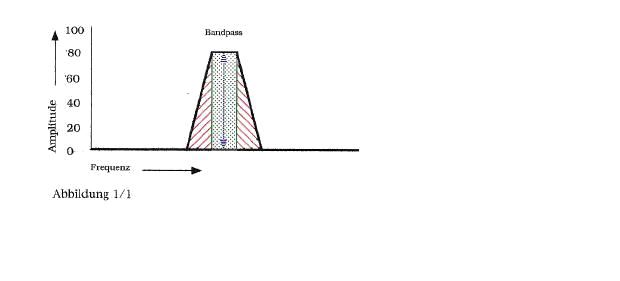
\includegraphics[width=1\textwidth]{images/nono/hph/ab_v_01.jpg}
\caption{}
\label{hph-img1}
\end{center}
\end{figure}

Mentre i due musicisti ed io abbiamo condotto i nostri esperimenti acustici, Luigi Nono deve aver aperto la porta del nostro studio e ascoltato gli esperimenti. All'improvviso entrò inaspettatamente, sorrise e disse: sono arrivato dopo tutto.
Poi ha annotato i risultati tecnici e sonori e come sono stati creati. Soprattutto Roberto ha dovuto mostrargli il suo nuovo flauto contrabbasso. Nono studiò i singoli campi di tono e suono, mise i suoi appunti nella sua borsa e disse: Devo tornare all'Halden-Hotel e continuare a lavorare. E quello stesso pomeriggio e sera, Luigi Nono ha composto le prime battute per "A Pierre", che ha provato, corretto e perfezionato con i musicisti e i tecnici dello Experimental Studio il giorno successivo.
Tornato a Venezia Nono finì immediatamente la versione finale di "A PIERRE", la prima esibizione avvenne pochi giorni dopo il 26 marzo 1985 a Baden-Baden, in occasione del 60 ° compleanno di Boulez.
Quindi, fate la genesi di Luigi Nonos A Pierre. Nono aveva studiato i nostri esperimenti sonori con molta attenzione e integrato nel suo nuovo lavoro in una forma completamente nuova. Il tempo di ritardo 12 e 24 secondi sono stati adottati da lui. Ha fatto uso del fatto che il suono della ripetizione filtrata e poco riverberata è andato ad estendere lo strato dopo 12 secondi.

\begin{figure}[htbp]
\begin{center}
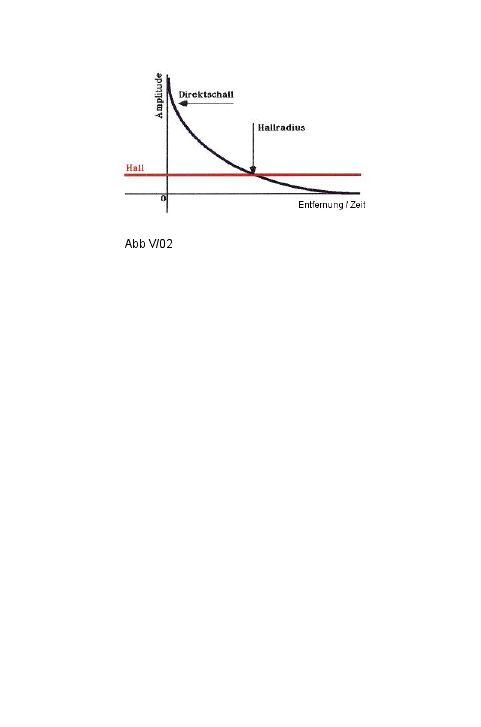
\includegraphics[width=1\textwidth]{images/nono/hph/ab_v_02.jpg}
\caption{}
\label{hph-img2}
\end{center}
\end{figure}

Conosciamo questo processo acustico come eco radiale, immagine 2. Con la diminuzione della dinamica del suono diretto e l'identica intensità del riverbero, percepiamo psicologicamente il suono diretto sempre più diffusamente in una distanza crescente. Questa estensione dello spazio sonoro diventa più chiara dalla trasformazione del suono diretto, dalla selezione del suono. Accanto al suono originale degli strumenti ci sono altri due livelli sonori, che sono enfatizzati dal loro ritardo di 12 e 24 secondi. Questa non è una dinamica, ma come accennato prima, un'estensione dello spazio dell'immagine sonora.
Nono sapeva dai nostri esperimenti a Friburgo, che questo poteva essere realizzato con un'idea musicale speciale e creato una forma di composizione strettamente orizzontale.

\begin{figure}[htbp]
\begin{center}
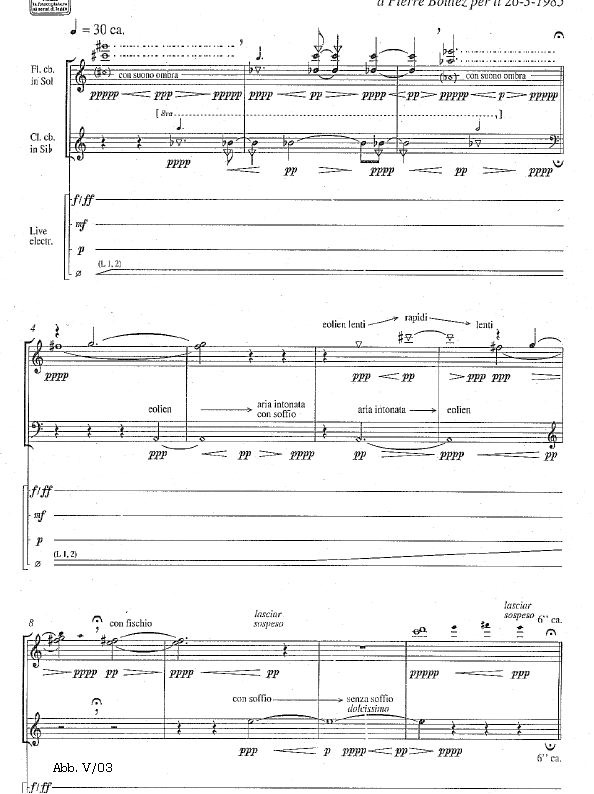
\includegraphics[width=1\textwidth]{images/nono/hph/ab_v_03.jpg}
\caption{}
\label{hph-img3}
\end{center}
\end{figure}


A prima vista, la partitura appare molto semplice, ma chiunque abbia studiato l'eccellente introduzione a A PIERRE nella Ricordi - avrà notato che Nono richiede per quasi ogni nota una forma di interpretazione individuale: dal fischio al fischietto. Per questo motivo, posso raccomandare lo studio di questi testi in tre lingue: italiano, inglese e tedesco.
Nono crea strutture sonore piene di contrasti che, secondo il tono, variano da suoni e toni pacifici ad aggressivi. Oltre a questo, il compositore ha utilizzato una trasformazione del suono per gli strumenti. Questa trasformazione - un piccolo sept e un tritone più basso - era guidata da un yy slow vibrato, che portava a un controllo variabile del pitch. Al fine di evitare un effetto sirena, questa trasposizione deve essere controllata molto dolcemente. Questa ricchezza di schemi sonori di entrambi gli strumenti suona insieme alla selezione del suono nei filtri passa banda e la trasformazione del suono crea nuovi spettri sonori molto interessanti, che - come mostrato nella figura 3 - possono essere ascoltati nella forma orizzontale di composizione di Nono in tutte le sottigliezze e vari livelli di suoni.
Certamente, Luigi Nono aveva già utilizzato materiali sonori simili per gli strumenti in "Amendes Klarsein" o in "Prometeo", ma insieme alla legenda tecnica finale come mostrato nel diagramma 4, il compositore realizza un'espressione musicale completamente nuova.

\begin{figure}[htbp]
\begin{center}
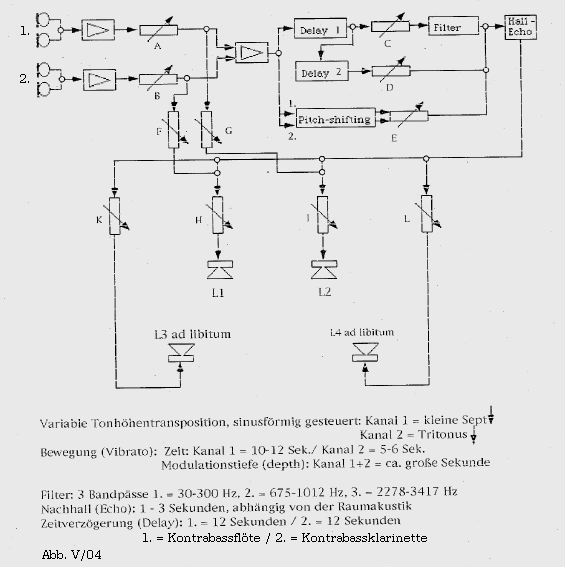
\includegraphics[width=1\textwidth]{images/nono/hph/ab_v_04.jpg}
\caption{}
\label{hph-img4}
\end{center}
\end{figure}

I singoli valori per il controllo dinamico e il tempo di riverbero sono indicati in percentuali relative e devono essere adattati all'acustica individuale della sala da concerto. La dinamica di Nono spazia da 5 pianissimos a forte, dove l'eruzione al forte appare solo una volta. Il più delle volte il volume varia attorno al pianissimo. Nono sviluppò ulteriormente la mia concezione di base dei miei esperimenti per evitare la ripetizione canonica udibile. Sulla base dei fermati a ripetizione continua di circa 6 secondi, la sequenza rigida di ripetizioni di 12 e 24 secondi si dissolve completamente. Così Nono impedisce una periodicità all'interno della sua musica che spesso si rivela molto differenziata e non ritmica, la cui forma interiore è composta in funzione del tempo. Pertanto, la direzione del suono deve essere così trasparente che l'ascoltatore non può verificare ciò che viene riprodotto in origine o ciò che viene riprodotto dagli altoparlanti. Due altoparlanti collocati dietro i solisti sono stati forniti per una performance. Successivamente, Nono collocò due altoparlanti aggiuntivi sul retro dell'auditorium, soprattutto nelle grandi sale da concerto, con la nota esplicita "ad libitum". Inoltre, il volume di questi 2 altoparlanti aggiuntivi 3 e 4 - dopo gli esperimenti con il compositore - deve essere controllato separatamente dagli altoparlanti 1 e 2. Il diagramma 5 mostra la relazione di dinamica tra gli altoparlanti.

\begin{figure}[htbp]
\begin{center}
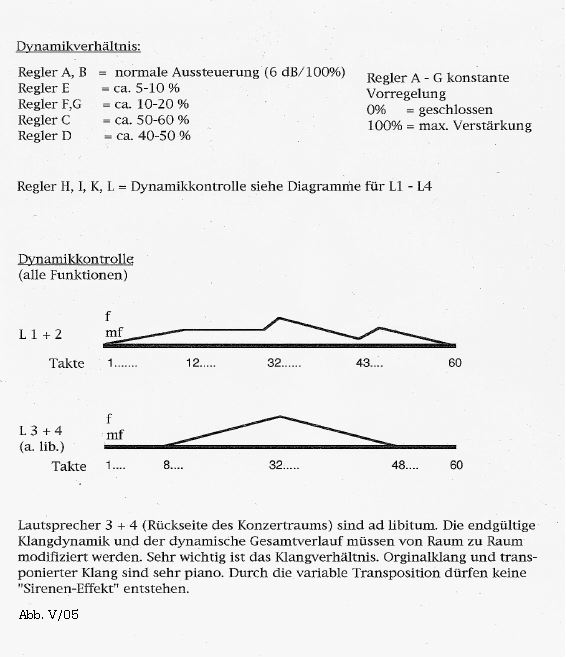
\includegraphics[width=1\textwidth]{images/nono/hph/ab_v_05.jpg}
\caption{}
\label{hph-img5}
\end{center}
\end{figure}

C'è stato il rimprovero che Live-Electronics, la trasformazione elettronica del suono sarebbe attributi di una composizione, che era stata aggiunta dopo il completamento del lavoro. Penso che non ci siano più composizioni tipiche di A Pierre e Omaggio a György Kurtag di Luigi Nono, che sconfiggono totalmente questo rimprovero. In entrambi i lavori, Nono ha incluso nel suo processo compositivo Live-Electronic come materiale equivalente accanto a strumenti meccanici tradizionali o voci. Entrambe le opere perderebbero la loro sostanza musicale senza l'estensione elettronica.
Lo sperimenteremo soprattutto nella recensione di Omaggio a György Kurtag. Per questo ora ho preparato un piccolo esempio con flauto solo. Innanzitutto, ascolterai un paio di battute da "A Pierre" senza Live-Electronics, quindi la stessa parte con estensione sonora elettronica:

Gli esempi sonori sono in mono. Il download completo è necessario prima dell'ascolto.

suono esempio 1 (Martin Fahlenbrock, flauto contrabbasso)
suono di esempio 2

Ci sono esempi che mostrano chiaramente che senza la transistor elettronica del suono, l'estensione del suono, uno strumento, manca una parte della sostanza compositiva. Come ho detto prima, dagli esperimenti di Freiburger, Nono sapeva esattamente i risultati sonori delle doppie ripetizioni, originali e trasformati. Ha composto le note degli strumenti con questo risultato, creando così una perfetta armonia tra meccanica e strumento elettronico. Non nego che ci siano composizioni, ad esempio Emmanuel Nunes: "Wandlungen", che può essere eseguita con e senza Live-Electronics. Tuttavia ciò non è possibile con le opere di Nonos create in collaborazione con Experimental Studio. Esigono un equilibrio tra i suoni degli strumenti tradizionali e i suoni della trasformazione elettronica. Di conseguenza non è possibile organizzare né nelle parti strumentali né nelle parti vocali e tecniche senza distruggere il suono che il compositore aveva puntato all'originale.

Ascoltiamo ora una sezione di "A Pierre" di Luigi Nono in una registrazione subito dopo il completamento della composizione, realizzata nel Freiburg Experimentalstudio (flauto di contrabbasso Roberto Fabbriciani e clarinetto contrabbasso Ciro Scarponi).

suono di esempio 3

\section{OMAGGIO A GYÖRGY KURTÁG}

La prima rappresentazione di "Omaggio a György Kurtág" il 10.6.83 a Firenze è stata una delusione per molti ascoltatori. È stata davvero una prima esibizione?
Nono stava lavorando a "Guai ai gelidi mostri" e "Prometeo" in quell'anno. Molte prove sperimentali hanno avuto luogo con la cantante Susanne Otto, lo strumentista Roberto Fabricciani, Ciro Scarponi e Giancarlo Schiaffini nello studio di Friburgo, una di queste prove è stato il concerto a Firenze. La composizione "Omaggio a György Kurtág" consisteva in valori soglia musicali, che Nono aveva indicato per ogni interprete in tono, spettri sonori e dinamici. Il compositore aveva anche dato alcuni suggerimenti per la tecnica della trasformazione del suono, che, tuttavia, non aveva nulla da fare con la versione finale di "Omaggio". Va detto che Luigi Nono, Alvise Vidolin e io - con la collaborazione dei musicisti - avevamo presentato una introduzione sulla trasformazione del suono elettronico all'inizio del concerto. Vorrei dire che la performance è stata un concerto di lavoro con il titolo: Composizione in corso. Nono non ha tratto profitto da questa esperienza in concerto fino alla sua composizione "Post-Prae-Ludium Donau" del 1987 per tuba solo e live-electronics. In questa composizione, per il musicista, valori di soglia, altezza, spettro sonoro, strutture ritmiche, scale di toni, volume e, soprattutto, sono state definite le strutture temporali. Gli intervalli devono essere riempiti dall'interprete mediante improvvisazioni. Sono indicati funzioni sonore e programmi per l'elettronica.
Quello che sto per dire ora si riferisce esclusivamente alla versione di "Omaggio", che è stata eseguita per la prima volta a Torino, il 6 giugno 1986.
All'inizio della mia conferenza scrissi: composizioni, in cui Luigi Nono aveva integrato in modo stringente una funzione estesa del tempo. Per A Pierre, Nono applica un ritardo di segnali acustici nel tempo, ripetizioni senza feedback. Sebbene questi determinino formalmente la composizione, l'idea di base di "Omaggio a György Kurtag" era completamente diversa.
Nono mi aveva comunicato il suo primo schizzo in una lettera:

\begin{figure}[htbp]
\begin{center}
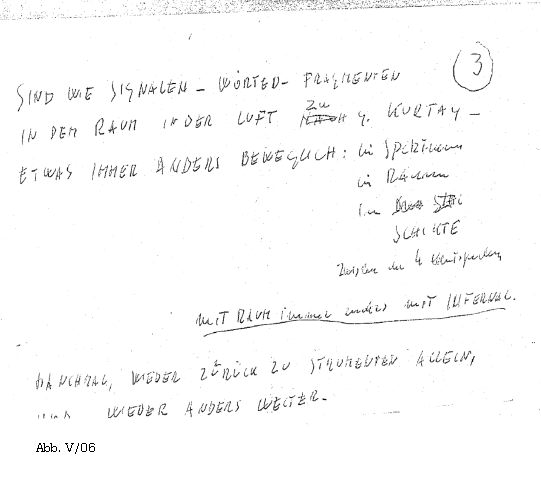
\includegraphics[width=1\textwidth]{images/nono/hph/ab_v_06.jpg}
\caption{}
\label{hph-img6}
\end{center}
\end{figure}

Cosa significa questo?
1.) La musica dovrebbe essere come segnali, parole, frammenti nell'aria, in
spazio a György Kurtag.
2.) Riguardo l'uso della trasformazione del suono elettronico Nono scrive:
Sempre nuovo, mai rigido, ma
cambio dello spettro, filtro passa banda,
cambiamento del suono dello spazio, varie posizioni del suono (4 altoparlanti), movimenti del suono, (esteso a 6 altoparlanti durante le prove),
La modifica del feedback significa feedback diverso al ritardo dei segnali.
3:) A volte solo strumenti, nient'altro che il suono strumentale e vocale originale.
4.) E ancora con live-electronics.
Per capire meglio, daremo un'occhiata alla foto 7, la leggenda tecnica, che ho registrato in questa forma durante le prove a Torino.

\begin{figure}[htbp]
\begin{center}
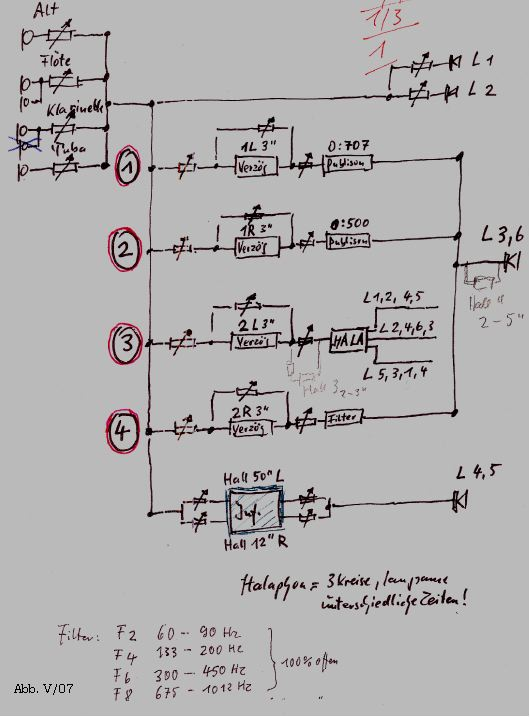
\includegraphics[width=1\textwidth]{images/nono/hph/ab_v_07.jpg}
\caption{}
\label{hph-img7}
\end{center}
\end{figure}

Per evitare equivoci, ho chiamato i programmi con combinazioni. Tutti e quattro sono ritardati di 3 secondi, con e senza feedback. A seconda della dinamica del feedback, i segnali di ingresso degli strumenti e la voce si attenuano in modo diverso. Al massimo una miscela di suoni nell'apparecchiatura di ritardo può essere memorizzata acusticamente per un periodo di tempo più lungo, alimentando le scale parzialmente orizzontali dei suoni originali sovrapposti, compressi e trasformati in una struttura verticale del suono. Nella sua lettera, Nono lo chiama: cambiamento nel feedback, che significa volume di feedback. Il cambiamento dello spettro sonoro - Nono non solo può ascoltarli durante le prove, ma anche vederli tridimensionalmente su uno schermo e battere con precisione - queste mutazioni sonore sono ottenute da tre possibilità:

1.) suddivisione dello spettro sonoro nei suoi singoli toni parziali. Conosciamo queste selezioni dalla prima ripetizione su A Pierre.
2.) Trasposizione di spettro in un harmonizer. Per "Omaggio" Nono ha scelto la trasposizione di un tritone e un'ottava più in basso. Mescolato con il suono originale, viene creato un nuovo spettro sonoro, dipendente dal volume di trasposizione.

Da un lato, lo spazio sonoro è cambiato da varie classi con i segnali di uscita ai 6 altoparlanti, dall'altro un movimento sonoro '150; ricorda alla combinazione tre. I movimenti sonori sono realizzati in tre diverse direzioni di movimento lente con un'apparecchiatura di controllo dello spazio sonoro universale, l'halaphone e sono definiti con precisione dal compositore. I singoli movimenti di direzione sono controllati tramite altoparlanti.
Fin dall'inizio, Luigi Nono ha avuto un'idea molto precisa dell'uso della trasformazione del suono elettronico per la sua composizione, che poi è stata resa più precisa durante le prove, Confrontiamo ancora una volta le figure 7 e 6.

Immagine 6

Immagine 7

Spectre - combinazione 4 , 5 filtri passa banda

spettro - combinazione 1 e 2 , trasformazione del suono

Combinazione 3- spazio - classificazione di altoparlanti, movimento del suono
Riverbero (12 + 50 secondi)

Feedback: ritardo di tre secondi con vari feedback

Corrispondente al suo schizzo tecnico, Nono ha composto la voce e la partitura strumentale:

Contrariamente a una forma prevalentemente verticale di Pierre, soprattutto alla realizzazione del lungo riverbero e dei suoni compressi dal feedback.

\begin{figure}[htbp]
\begin{center}
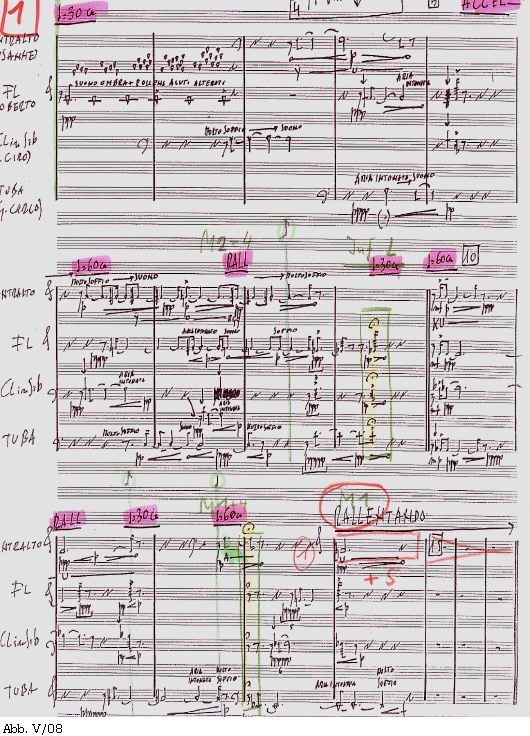
\includegraphics[width=1\textwidth]{images/nono/hph/ab_v_08.jpg}
\caption{}
\label{hph-img8}
\end{center}
\end{figure}

Nella figura 8 vediamo la prima pagina della partitura scritta a mano con note supplementari di controllo del suono, prima esecuzione, Torino. Nella barra 9, contrassegnata in verde, l'accordo dello strumento di ottone viene riverberato artificialmente per 50 secondi. Naturalmente, l'intensità di questo accordo - pianissimo - accorcia molto il riverbero. La durata del riverbero dipende dall'intensità del segnale di ingresso. Pertanto, Nono non indica una durata esatta, ma collega questo riverbero tecnicamente inesatto da un arresto. Ma ciò che può essere ascoltato, tuttavia, è il volume del suono, che corrisponde alla dimensione di una stanza geometrica di 50 secondi. Pertanto è importante che vengano utilizzate solo apparecchiature di ritardo con un volume di spazio controllato. La suddetta fermata consente al controllo del suono di variare in modo variabile attenuando il tempo di riverbero in base alle dimensioni della sala da concerto. Gli intervalli sonori realizzano lo schizzo di Nono. "come segnali a György Kurtag" Dove troviamo un intervallo sonoro più breve nella battuta 13, Nono impiega la prima versione di un intervallo sonoro di delay con feedback per il contralto nella barra da 14 a 17. Il tempo prescritto è un quarto di nota uguale a 60 , il tempo di ritardo con feed-back di 3 secondi. Con una mezza nota del contralto, si ottiene una ripetizione con un semplice feedback. La funzione di fadeout altrettanto breve del feedback è contrassegnata in rosso. Il suono originale della voce viene trasposto nel delay di un tritone in basso (combinazione 1).

\begin{figure}[htbp]
\begin{center}
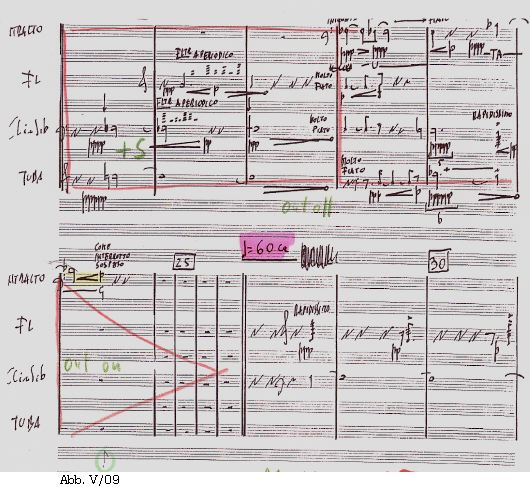
\includegraphics[width=1\textwidth]{images/nono/hph/ab_v_09.jpg}
\caption{}
\label{hph-img9}
\end{center}
\end{figure}

Nelle barre 18-20, Nono impiega la seconda versione dell'intervallo sonoro per ritardo con feedback. Tuttavia, vista formalmente, questa versione è completamente cambiata rispetto alla battuta 14. Il suono originale degli strumenti di ottone viene di nuovo ritardato di tre secondi con un feedback e una trasposizione di un tritone più in basso. Il risultato non può essere ascoltato immediatamente, ma viene riprodotto nella battuta 23 -27. Questo effetto acustico può essere chiamato eco con una lunga riverberazione, ovvero l'intensificazione del suono della barra 18-20 può essere percepita solo 20 secondi dopo. Un'idea compositiva, che combina due funzioni temporali in un unico complesso: durata della ripetizione con feedback e durata dell'eco. Nell'esempio 4, prima ascolteremo lo spazio sonoro ingrandito e il riverbero sovradimensionato.

suono di esempio 4

Il feedback è stato sbiadito. Nell'esempio seguente, ascolteremo un ritardo con feedback, formiamo uno senza cambiamenti nel tempo. Vorrei richiamare la tua attenzione sulla trasposizione in un tritone più in basso.

suono di esempio 5

La terza versione, il suono originale compresso e trasposto con riproduzione indietro spostato nel tempo. Il feedback si attenua lentamente, c'è un naturale sbiadimento dovuto alla dissoluzione della densità del suono. Questa procedura tecnica è particolarmente importante per una performance.

esempio sonoro 6

Questi esempi sonori sono continuamente modificati - come sappiamo dalla leggenda tecnica - durante l'intero lavoro. Così il compositore realizza il suo concetto: "Qualcosa è continuamente e diversamente flessibile"

La restante parte di voce e strumento rimane invariata senza la trasformazione del suono. Con questo, Luigi Nono enfatizza la funzione di live-electronic, gli intervalli sonori creano nuove dimensioni del suono e del tempo. Citazione del compositore: nello spazio cosmico verso l'universo, altri spazi, altre terre, altri abissi, altre fantasie. (Fine della citazione).
Con questi due lavori, "A Pierre" e "Omaggio a György Kurtág", Luigi Nono ha scoperto nuovi strati sonori, che ha potuto realizzare con l'aiuto della tecnica moderna, la trasformazione elettronica del suono. Sebbene diversi negli strumenti, diversi nella forma della composizione, entrambe le opere hanno un significato comune, un concetto spirituale comune.

Ascoltiamo "Omaggio a György Kurtag" due volte. Durante il primo replay, ti mostrerò il punteggio sullo schermo, per dimostrare cosa intendevo mostrare. prima. Poi ascolteremo il breve brano, circa 15 minuti, ascolteremo la musica di Nono, senza essere distratti dalle impressioni visive. Quest'opera di Nono è stata pubblicata in un'ottima edizione dalla casa editrice Ricordi. Sto usando una copia della partitura originale, poiché ho usato i colori per tutte le funzioni di live-electronic durante le prove per la prima esibizione a Torino.

Esempio 7 (con schermo)
Esempio 8 (senza schermo) Si prega di ascoltare gli esempi 7 e 8 dal CD "luigi nono 3", AUVIDIS FRANCE, MO 782047.


%!TEX TS-program = xelatex
%!TEX encoding = UTF-8 Unicode
% !TEX root = ../../2017-GS-COME01-INVITO-ASCOLTO.tex

\clearpage

\thispagestyle{empty}

\includepdf[scale=1.05,
		    pagecommand={
		    	\begin{tikzpicture}[
					remember picture,
					overlay]
		    	\node [xshift=2cm,yshift=1cm] at (current page.south west) {\color{white}{\emph{Roberto \textbf{Masotti}}}};
				\end{tikzpicture}}
		    ]{images/lucier/lucier_road_cc.pdf}

\clearpage

%-------------------------------------------------------------
%---------------------- ALVIN LUCIER - I'M SITTING IN A ROOM -
%-------------------------------------------------------------

\chapter*{1998. Alvin LUCIER. \\ \emph{Waves Song}.}
\addcontentsline{toc}{chapter}{1998. Alvin LUCIER. \emph{Waves Song}.}

	\begin{flushright}
		\textit{Nella nostra anima c'è una incrinatura che, se sfiorata, \\
		risuona come un vaso prezioso riemerso dalle profondità della terra} \\
		Wassilly Kandinsky - \emph{Lo Spirituale nell'Arte}
	\end{flushright}

	\begin{flushright}
		\textit{Music of Changes // John ChAnGEs} \\
		Pierre Boulez
	\end{flushright}

	\begin{flushright}
		\textit{Si dice che i compositori abbiano orecchio per la musica e \\
		di solito significa che non sentono nulla che arrivi alle loro orecchie. \\
		Le loro orecchie sono murate dai suoni di loro creazione.} \\
		John Cage - \emph{45' for a Speaker} (1954)
	\end{flushright}

\bigskip

\section*{Ever Present}

%\begin{multicols}{2}

\begin{quote}
	On 24 September 1960, I attended a concert by John Cage, David Tudor, Merce Cunningham and Carolyn Brown at La
	Fenice Theater in Venice. I had come to Venice that summer on a Fulbright Scholarship to study at the Benedetto
	Marcello Conservatory before going on to Rome where I would spent the next 2 years. The Cage-Tudor event came
	like a bolt out of the blue-all the protocols of the concert situation were violated.
	The concert began, as I remember, with David Tudor striding down the aisle of the theatre and diving under
	the piano, hitting the underside to make the first sound of the concert. Cage made an appearance playing
	a piano that rose up into the pit hydraulically. The four per- formers had cards upon which were written instructions
	regarding sound s or actions to be made and where to make them. The entire theatre was used-stage, aisles, balconies.
	The work was \emph{Music Walk with Dancers} (1958). During that concert a man walked down the aisle and struck the piano
	with an umbrella and announced: "Now I am composer!" At the height of the pandemonium, Cage was tuning a radio
	that he used as a sound source, and the Pope came on asking for peace on earth.

	That concert forever altered the way I thought about mu- sic. Until that time I had followed the conventional pattern of
	composer-performer-audience relationships. One would compose a work, wait for some soloist, ensemble or orchestra to perform it, then hope that the audience would like it. It was a lonely life; a waiting game.
\end{quote}

di John Cage, in luogo degli antichi Greci, come avrebbe continuato Kandinsky.
Ci deve essere un certo grado di consapevolezza in relazione al livello di
comprensione-incomprensione del pensiero di John Cage. Ma ammettendo di
averlo compreso, per quanto noi potremmo approfondire lo studio del suo
pensiero e della sua musica, potremmo solo arrivare ad imitarne alcuni tratti
stilistici. E se tentassimo di

\begin{lstlisting}[style=SuperCollider-IDE]
// oscillazione sinistra che sale
// questa deve uscire sul canale 1
{ SinOsc.ar(
  Line.kr(
    start: 60.midicps,
    end: 84.midicps,
    dur: 504,
), 0, 0.5) }.play;

// oscillazione destra che scende
// questa deve uscire sul canale 2
{ SinOsc.ar(
  Line.kr(
    start: 60.midicps,
    end: 56.midicps,
    dur: 252,
), 0, [0, 0.5]) }.play;

// come far suonare eventi in successione?

//   UP da c3 a c4 in 252
// DOWN da c3 a aes2 in 252
{ SinOsc.ar([Line.kr(60.midicps, 72.midicps, dur: 252), Line.kr(60.midicps, 56.midicps, dur: 252)], 0, 0.5) }.play;

//   UP da c3 a c4 in 252
// DOWN da c3 a aes2 in 252
{ SinOsc.ar([Line.kr(72.midicps, 84.midicps, dur: 252), Line.kr(56.midicps, 47.midicps, dur: 252)], 0, 0.5) }.play;

(
  SystemClock.sched(0.0,{
    "00:00 starting point".postln;
    x = SynthDef.new("sinosc", { Out.ar(0, SinOsc.ar([Line.kr(60.midicps, 72.midicps, 252), Line.kr(60.midicps, 56.midicps, 252.1)], 0, 0.5))}).play;
    nil;
});

  SystemClock.sched(252.0,{
    "252 bottom cue".postln;
    x.free;
    y = SynthDef.new("sinosc", { Out.ar(0, SinOsc.ar([Line.kr(72.midicps, 84.midicps, 252), Line.kr(56.midicps, 47.midicps, 252.1)], 0, 0.5))}).play;
    nil;
});

  SystemClock.sched(504.0,{
    "middle point".postln;
    y.free;
    nil;
});
  s.record(duration:504);
)
\end{lstlisting}

%\end{multicols}


%!TEX TS-program = xelatex
%!TEX encoding = UTF-8 Unicode
% !TEX root = ../../2017-GS-COME01-INVITO-ASCOLTO.tex

\clearpage

\thispagestyle{empty}

\includepdf[scale=1.03,
		    pagecommand={
		    	\begin{tikzpicture}[
					remember picture,
					overlay]
		    	\node [xshift=2cm,yshift=1cm] at (current page.south west) {\color{white}{\emph{Heinz \textbf{Karnine}}}};
				\end{tikzpicture}}
		    ]{images/stockhausen/stockhausen.pdf}

\clearpage

%-------------------------------------------------------------
%---------------------------- KARLHEINZ STOCKHAUSEN - MANTRA -
%-------------------------------------------------------------

\chapter*{1970. Karlheinz Stockhausen.\\\emph{Mantra}.}
\addcontentsline{toc}{chapter}{1970. Karlheinz Stockhausen. \emph{Mantra}.}

%	\begin{flushright}
%		\textit{Nella nostra anima c'è una incrinatura che, se sfiorata, \\
%		risuona come un vaso prezioso riemerso dalle profondità della terra} \\
%		Wassilly Kandinsky - \emph{Lo Spirituale nell'Arte}
%	\end{flushright}
%
%	\begin{flushright}
%		\textit{Music of Changes // John ChAnGEs} \\
%		Pierre Boulez
%	\end{flushright}
%
%	\begin{flushright}
%		\textit{Si dice che i compositori abbiano orecchio per la musica e \\
%		di solito significa che non sentono nulla che arrivi alle loro orecchie. \\
%		Le loro orecchie sono murate dai suoni di loro creazione.} \\
%		John Cage - \emph{45' for a Speaker} (1954)
%	\end{flushright}

\bigskip

\begin{multicols}{2}

In una presentazione del 2009 per la prima neozelandese di \emph{Mantra}, Robin Maconie traccia i collegamenti storici tra la genialità di Stockhausen e una serie di semine musicali che negli anni precedenti ne hanno costruito il background immaginifico.

Il primo nome che Maconie collega a Stockhausen è quello di Arnold Schoenberg, mettendo in relazione il gli intervalli iniziali di \emph{Mantra} con alcuni tratti melodici dell'inizio dell'\emph{Op. 11 N. 2} per pianoforte. Maconie mette in relazione la nota perno \emph{La} attorno alla quale si muovono formule simmetriche con l'\emph{Op. 27} di Webern e \emph{Music for String, Percussion e Celesta} di Bartok:

\begin{quote} The mirror-symmetry in both cases is significant, and also the date: both works were composed in 1936. For the postwar Darmstadt generation of serial composers, mirror-imagery takes the form of a symmetrical all-interval series, the utopian generative principle commended by Herbert Eimert, Stockhausen's mentor and coeditor of the periodical Die Reihe, and adopted by Boulez, Stockhausen, and Nono. [\ldots] In Mantra a listener is able to detect echoes and allusions to a western tradition of music-making.\footnote{La simmetria speculare in entrambi i casi è significativa, e lo è anche la data: entrambe le opere furono composte nel 1936. Per la generazione postbellica dei compositori serialisti di Darmstadt, le immagini speculari presero la forma di una serie simmetrica che contemplasse tutti gli intervalli, un principio generativo utopico proposto da Herbert Eimert, mentore e coeditore di Stockhausen del periodico \emph{Die Reihe}, e adottato da Boulez, Nono e Stockhausen stesso. [\ldots] In \emph{Mantra} l'ascoltatore è in grado di riconoscere gli echi e le allusioni alla tradizione musicale occidentale.}
\end{quote}

Il collegamento tra Stockhausen e Boulez passa anche per la costruzione formale, per gli sviluppi interni della struttura che si contrae ed espande per tutta l'estensione della tastiera all'interno delle tessiture musicali, che Maconie collega alle \emph{Structures} per due pianoforti del 1951-52.

L'ultima riflessione di Maconie sulle radici storiche di \emph{Mantra} è relativa alla presenza delle percussioni. I nomi che qui collega sono quelli di John Cage, che negli anni cinquanta raggiunge l'Europa con le sue sonorità pianistiche non convenzionali, e di Bela Bartok con la \emph{Sonata per due pianoforti e percussione} sulla quale nel 1951 Stockhausen redige la sua tesi di diploma musicale.


%1969 quattro persone che chiacchierano di questo e quello in una macchina tra medicine connecticut e boston.
%lungo la strada scrive su una busta che aveva in tasca una melodia che contiene tutte e dodici le note. un anno dopo
%inizia il suo lavoro per due pianoforti e riprende questa melodia.
%tutta la melodia stirata sull'intera durata del brano, un'ora. e contemporanemamente compressa nella più piccola portzione temporale.
%ogni nota a sua volta richiamava a se tutte le altre note rendendo per ognuno di questi punti il complesso delle 12 note. Il tutto somiglia
%molto ad un sistema di stelle.
%
%tutta la melodia è il mantra, come fosse una formula. ci sono 4 regioni separate da pause. la prima regione è formata da 4 note. la seconda da 2. la terza da 5 la quarta da 3
%
%mirror
%
%spiegherò come il mantra, la formula, può essere usata per l'intera composizione, per fare questo ho bisogno della variazione
%
%trovare qualcosa sulle lezioni inglesi?
%
%dobbiamo immaginare come se ogni nota determina un'intera sezione di una certa composizione
%
%combinare le sezioni tra loro con la tecnica delle variazioni
%
%non ho costruito la formula sulla base di una scala cromatica

%due note su mantra:
%
%\emph{perché le onde corte?} \\
%Stockhausen inizia a scrivere \emph{Mantra} durante la residenza giapponese di Osaka per il settantesimo Expo universale. Utilizza le onde corte nel 1968 per \emph{Kurzwellen} e \emph{Spiral} e proprio questo brano è cardine per la programmazione dei concerti Expo. La prima di \emph{Mantra} avviene al \emph{Donaueschingen Festival} con il duo Kontarksy nel 1970, dopo l'esperienza di Osaka. \emph{Mantra} è il primo brano in cui Stockhausen utilizza la \emph{formula}. L'idea di applicare la \emph{Ring Modulation} sui suoni di pianoforte proviene quindi dai precedenti lavori: \emph{Kurzwellen mit Beethoven} dove tra i vari suoni di Beethoven modula anche le sonate per pianoforte. Anche le onde corte provengono dai lavori di quel periodo, \emph{Kurzwellen} e \emph{Spiral}.

\end{multicols}

%http://www.sonoloco.com/rev/stockhausen/16.html
%http://stockhausenspace.blogspot.it/2014/06/opus-32-mantra.html
%http://stockhausenspace.blogspot.it/p/timeline-history-of-20th-century.html
%http://stockhausenspace.blogspot.it/p/year-biographical-info-from-official.html
%https://www.youtube.com/watch?v=Z8srbuxyIVw&feature=youtu.be
%http://www.staff.city.ac.uk/newton.armstrong.1/mantra/
%https://www.swr.de/swr-classic/donaueschinger-musiktage/programme/1970/-/id=2136962/did=3459926/nid=2136962/1b1tc0l/index.html

\begin{table}[htp]
\begin{center}
\begin{sf}{\footnotesize
\begin{tabular}{r c c c c c c c c c c c c c c c c c c }

       \textbf{altezze} & \multicolumn{4}{c}{4} 	 & \multirow{3}*{pausa 3} & \multicolumn{3}{c}{2} & \multirow{3}*{pausa 2} & \multicolumn{5}{c}{5}  & \multirow{3}*{pausa 1} & \multicolumn{3}{c}{3}  \\
\textbf{durata regione} & \multicolumn{4}{c}{10} &                        & \multicolumn{3}{c}{6} &                        & \multicolumn{5}{c}{15} &                        & \multicolumn{3}{c}{12}   \\
  \textbf{suddivisione} & 1 & 2 & 3 & 4          &                        & 2 & 2 & 2             &                        & 5 & 2 & 1 & 3 & 4      &                        & 4 & 2 & 6 \\

\end{tabular}}
\end{sf}
\end{center}
\caption{Melodia - Formula - Regioni}
\label{default}
\end{table}%


%----------------------

\begin{table}[htp]
\begin{center}
\begin{sf}{\footnotesize
\begin{tabular}{|c|l|c|c|}

\hline
& Andamento musicale & Battuta iniziale & Nota di partenza \\
\hline
\hline
1 & Ripetizione regolare & 12 & La \\
\hline
2 & Accento alla fine & 61 & Si \\
\hline
3 & \emph{Normale} & 89 & Sol\# \\
\hline
4 & gruppetti e acciaccature attorno ad un tono centrale & 125 & Mi \\
\hline
5 & Tremolo & 205 & Fa \\
\hline
6 & Accordo (accentato) & 282 & Re \\
\hline
7 & Accento all'inizio & 445 & Sol\# \\
\hline
8 & Connessione cromatica & 488 & Mi\emph{b} \\
\hline
9 & Staccato & 538 & Re\emph{b} \\
\hline
10 & Ripetizioni irregolari (Codice \emph{Morse}) & 587 & Do \\
\hline
11 & Trilli & 611 & Si\emph{b} \\
\hline
12 & Accento \emph{Sforzando} & 641 & Sol\emph{b} \\
\hline
13 & Arpeggio come connessione & 673 & La \\
\hline

\end{tabular}}
\end{sf}
\end{center}
\caption{\emph{Mantra} consta di 13 grandi sezioni derivanti dalle 13 note della formula. Ogni sezione tratta un particolare andamento musicale, anch'esso derivato dal mantra.}

\label{default}
\end{table}%


%----------------------

\begin{table}[htp]
\begin{center}
\begin{sf}{\footnotesize
\begin{tabular}{|c|c|c|c|c|c|c|c|c|c|c|c|c|c|}

\hline
  & \textbf{I} & \textbf{II} & \textbf{III} & \textbf{IV} & \textbf{V} & \textbf{VI} & \textbf{VII} & \textbf{VIII} & \textbf{IX} & \textbf{X} & \textbf{XI} & \textbf{XII} & \textbf{XIII} \\
  \hline
  \hline
\textbf{1} & 12 & 61 & 89 & 125 & 205 & 282 & 446 & 488 & 540 & 587 & 611 & 641 & 673 \\
\hline
\textbf{2} & 56 & 85 & 122 & 198 & 276 & 318 & 486 & 535 & 538 & 609 & 630 & 671 & 871 \\
\hline
\textbf{3} & 12 & 61 & 102 & 125 & 209 & 286 & 447 & 492 & 582 & 590 & 612 & 661 & 676 \\
\hline
\textbf{4} &  53 & 83 & 121 & 195 & 268 & 318 & 478 & 530 & 570 & 608 & 628 & 668 & 868 \\
\hline
\textbf{5} & 46 & 81 & 114 & 192 & 262 & 312 & 450 & 526 & 567 & 594 & 626 & 665 & 865 \\
\hline
\textbf{6} & 26 & 75 & 91 & 146 & 257 & 311 & 454 & 525 & 563 & 603 & 620 & 634 & 855 \\
\hline
\textbf{7} & 29 & 79 & 110 & 189 & 262 & 300 & 452 & 508 & 556 & 607 & 624 & 665 & 862 \\
\hline
\textbf{8} & 19 & 71 & 97 & 128 & 245 & 296 & 472 & 496 & 544 & 599 & 616 & 656 & 681 \\
\hline
\textbf{9} & 22 & 73 & 100 & 201 & 280 & 304 & 466 & 502 & 540 & 609 & 618 & 659 & 685 \\
\hline
\textbf{10} & 59 & 87 & 124 & 132 & 246 & 325 & 458 & 537 & 586 & 610 & 632 & 672 & 872 \\
\hline
\textbf{11} & 30 & 77 & 105 & 152 & 259 & 308 & 486 & 521 & 548 & 603 & 622 & 663 & 858 \\
\hline
\textbf{12} & 13 & 69 & 92 & 127 & 212 & 292 & 448 & 493 & 562 & 592 & 614 & 651 & 679 \\
\hline

\end{tabular}}
\end{sf}
\end{center}
\caption{Tabella dei 156 \emph{mantra} (battute di inizio). La riga con le cifre romane indica le tredici sezioni mentre la prima colonna numera le dodici suddivisioni in sezioni. Da questa visualizzazione si possono notare alcune particolari condizioni come per esempio la partenza delle espansioni I.1 e I.3 alla stessa battuta. (da Richard Toop, \emph{Six Lectures from the Stockhausen Courses Kurten 2002})}

\label{default}
\end{table}%

\begin{lstlisting}[style=SuperCollider-IDE]
SynthDef('shortwave', {
	var level, sw1, sw1_d, sw1_f, sw1_t, sw2, sw2_d, sw2_t;

	level = Lag3.kr(In.kr(2).linlin(0, 1, -30, 0), 0.1).dbamp;

	sw1_d = Drand(({ rrand(0.02, 0.04) } ! 23), inf);
	sw1_t = Duty.kr(sw1_d, 0, Dseq([1, 0], inf));
	sw1_f = TChoose.kr(sw1_t, [1240, 2400, 2450]) + ({ LFDNoise3.kr(0.3, 40) } ! 3);
	sw1 = SinOsc.ar(Lag3.kr(sw1_f, 0.01), 0, LFDNoise3.kr(0.3).range(-36, -24).dbamp);
	sw1 = sw1 * Lag3.kr(Trig.kr(sw1_t, sw1_d), 0.01);
	sw1 = PitchShift.ar(sw1, 0.1, 1, 0.005, 0.005);

	sw2_d = Dxrand([0.6] ++ ({ rrand(0.02, 0.09) } ! 15), inf);
	sw2_t = Duty.kr(sw2_d, 0, Dseq([1, 0], inf));
	sw2 = SinOsc.ar(960 + LFDNoise3.kr(0.2, 25), 0, -21.dbamp);
	sw2 = sw2 * Lag3.kr(Trig.kr(sw2_t, TWChoose.kr(sw2_t, [0.04, 0.09], [0.7, 0.3])), 0.005);

	Out.ar(4, Mix([sw1, sw2]) * level);
}).add;
\end{lstlisting}


%!TEX TS-program = xelatex
%!TEX encoding = UTF-8 Unicode
% !TEX root = ../../2017-GS-COME01-INVITO-ASCOLTO.tex

\clearpage

\thispagestyle{empty}

\includepdf[offset=-10 0,
			scale=2.15,
		    pagecommand={
		    	\begin{tikzpicture}[
					remember picture,
					overlay]
		    	\node [xshift=4cm,yshift=1cm] at (current page.south west) {\color{white}{\emph{\textbf{Massimo Cacciari} e \textbf{Luigi Nono}, Venezia 1983}}};
				\end{tikzpicture}}
		    ]{images/nono/luigi-nono-massimo-cacciari.pdf}

%Massimo Cacciari e Luigi Nono, Venezia 1983.

\clearpage

%-------------------------------------------------------------
%------------------------------------- GINC - OMAGGIO SCELSI -
%-------------------------------------------------------------

\chapter*{1976. GINC.\\\emph{Omaggio a Scelsi}.}
\addcontentsline{toc}{chapter}{1976. GINC. \emph{Omaggio a Scelsi}.}


%!TEX TS-program = xelatex
%!TEX encoding = UTF-8 Unicode
% !TEX root = ../../2017-GS-COME01-INVITO-ASCOLTO.tex

\clearpage

\thispagestyle{empty}

\includepdf[offset=-10 0,
			scale=2.15,
		    pagecommand={
		    	\begin{tikzpicture}[
					remember picture,
					overlay]
		    	\node [xshift=4cm,yshift=1cm] at (current page.south west) {\color{white}{\emph{\textbf{Massimo Cacciari} e \textbf{Luigi Nono}, Venezia 1983}}};
				\end{tikzpicture}}
		    ]{images/nono/luigi-nono-massimo-cacciari.pdf}

%Massimo Cacciari e Luigi Nono, Venezia 1983.

\clearpage

%-------------------------------------------------------------
%---------------------- LUIGI NONO - OMAGGIO A GYORGY KURTAG -
%-------------------------------------------------------------

\chapter*{1983. Luigi Nono.\\\emph{Omaggio a György Kurtág}.}
\addcontentsline{toc}{chapter}{1983. Luigi Nono. \emph{Omaggio a György Kurtág}.}

La lista delle opere di un autore disegna un percorso, una trama. Al suo interno una fitta rete di relazioni tra scelte ed occasioni, tra progetti e potenzialità che collega per grado congiunto il filamento del DNA dell'autore stesso. Non solo un filo cronologico bidirezionale ma una molteplicità di connessioni che ad ogni passo, ad ogni titolo aggiunto, cristallizza una fitta trama di riferimenti storici e sociali che si dipana nel tempo, che ripercorre un sentiero fino alla sorgente e contemporaneamente spinge il percorso verso un'idea di futuro. 

Studiando il repertorio, focalizzando il breve periodo che porta all'opera analizzata, che la precede ed immediatamente segue, intessendo ai testi musicali i testi letterari, le interviste e gli scritti, si può ricostruire il processo compositivo di sentimenti e trasformazioni, di scelte ed obiettivi che ha portato il pensiero musicale alla scoperta di quella composizione, o un numero di composizioni in un dato periodo.

I riferimenti cronologici ci permettono di fissare punti sulla mappa temporale mentre i singoli percorsi a definire il disegno storico. È indispensabile applicare questo ragionamento internamente ad ogni singolo autore, per apprenderne il più intimo percorso, quanto alla relazione tra gli autori, o meglio, tra le loro opere, al fine di comprenderne il punto inesatto nel contesto storico, piuttosto che il punto esatto della catalogazione storica. 

\begin{quote}
\ldots Sarebbe quindi sbagliato dedurre lo sviluppo spirituale della musica dall'esatta cronologia delle opere. La considerazione storica della musica fino ai tempi nostri poggia sulle relazioni culturali-spirituali anziché su date enumerate\footcite[pag. 2 ]{fleischer:mcont}.
\end{quote}

Questo guardare costantemente alle relazioni, ai ruoli nello spazio e nel tempo, fanno costantemente ricorso ad una capacità di visione d'insieme, dall'alto, che attinga a coscienza storica, a quadro d'unione. L'analisi sull'opera contemporanea, la capacità di ridurre l'informazione istantanea all'intimo legame tra suono e pensiero, deve passare inevitabilmente per un \emph{pensare la musica oggi} di quell'oggi costantemente in un altro tempo del suo presente. 

\begin{quote}
L'Ottocento rappresenta certo il culmine dell'epoca borghese, ma subito, già nel medesimo secolo, comincia la decadenza. Il \emph{borgese} diventa man mano \emph{piccolo borghese}, la sua vita appare vuota, superficiale, monotona, il sentimento cosmico e il contatto intimo con la natura scompaiono; l'orizzonte spirituale si restringe in un ingranaggio quotidiano ormai meccanico e burocratico. Ciò che è piccolo, la forma, sorta da un mondo adattato all'occhio umano, diventa minimo. 

La visuale sul vasto mondo viene oscurata; l'interesse è rivolto al particolare. Il greto interessamento per la particella più minuta, l'incapacità di riconoscere il cosmo nel più minuto particolare, seguono la tragedia della borghesia morente. Teoria atomica e psicoanalisi costituirono i sintomi estremi della degenerazione spirituale: corpo e anima sono analizzati nelle più minuscole particelle, da cui devono ricostruirsi a guisa di mosaico. Nell'analisi va perduto ogni senso cosmico.
\end{quote}

Voglio usare questa capacità di collegare i punti per filare la trama attorno all'\emph{Omaggio}, risalendo, dove possibile, ricucendo gli strappi e le inopportune interpretazioni che il tempo contemporaneo possono aver generato.

\begin{compactitem}
  \item 1975.	\emph{Al gran sole carico d’amore per scena}
  \item 1976.	\emph{Al gran sole carico d’amore (frammenti)}
  \item 1976.	\emph{\ldots sofferte onde serene\ldots}
  \item 1976.	\emph{I turcs tal Friúl}
  \item 1979.   \emph{Con Luigi Dallapiccola}
  \item 1980.	\emph{Fragmente – Stille, An Diotima}
  \%item 1981.	\emph{Io, frammento dal Prometeo}
  \item 1981.	\emph{Das atmende Klarsein}
  \item 1982.	\emph{Quando stanno morendo. Diario polacco n. 2}
  \item 1982.	\emph{¿Donde estás hermano?}
  \item 1983.	\emph{Omaggio a György Kurtág}
  \item 1983.	\emph{Guai ai gelidi mostri}
  \item 1984.	\emph{A Carlo Scarpa, architetto, ai suoi infiniti possibili}
  \item 1984.	\emph{Prometeo. Tragedia dell’ascolto per scena}
\end{compactitem}

Si potrebbe definire questa lista di opere come un tratto, nel cammino di Nono, tra due spazi-tempo. È un mare che collega un'isola ad un'altra. È lo sguardo sul buio tra due stelle. Gli estremi, \emph{Al gran sole} e \emph{Prometeo}, di un silenzio.

\begin{quote}
[\ldots] un silenzio inesprimibile: non avevo cioè i mezzi adatti ad esprimermi. Contemporaneamente è iniziato il mio rapporto di amicizia con Massimo Cacciari che pure conoscevo dal 1965. Ho sentito una necessità di studio non solo sul mio linguaggio musicale ma anche di analisi delle mie categorie mentali e ho ripreso a comporre con \ldots \emph{sofferte onde serene} \ldots, un lavoro che mi ha impegnato moltissimo.
	
	Due o tre anni fa Ronconi mi chiese di andare a Prato per partecipare ai suoi incontri teatrali con gli attori e gli studenti del Laboratorio. Lì ho pensato per la prima volta al \emph{Prometeo}; ne ho parlato con Massimo che mi ha dato la prima stesura del testo.\footcite[vol. II p. 245, \emph{Intervista di Renato Garavaglia 1979-80}]{nono:scrcol}.
\end{quote} 

Una fase quindi, quella che va tra \emph{al gran sole} a \emph{prometeo} che vede, durante il percorso, la nascita di una nuova esigenza compositiva strutturata in un nuovo linguaggio e nuove categorie mentali. Un percorso che fa tappa a Friburgo, nello studio di Fonologia, dove queste nuove esigenze fioriscono in un nuovo metodo compositivo.

La visione di “luoghi” di suono, sonori, da raggiungere con il movimento spaziale è un'immagine radicata nell'idea musicale del \emph{Prometeo}.

\begin{quote}
	Mentre nel \emph{Gran Sole} c'è stato tutto un intersecarsi dei vari momenti, dei testi, ecc., qui ci sono come delle “isole” in continua trasformazione; ci sono dei continui viaggi tra queste “isole” che introducono nuove prospettive, nuove angolazioni conoscitive. Non ci sarà una successione, uno sviluppo tradizionale delle scene, ma tutta una sovrapposizione complessa, con ritorni, prospettive utopiche che si richiamano continuamente. Per adesso non mi interessa tanto un movimento scenico ma l'utilizzazione dello spazio in cui avviene l'esecuzione e come lo spazio può legare, comporre, slegare, i vari momenti e tutte le formanti musicali (voci, strumenti, ecc.). Penso di utilizzare il testo anche attraverso la programmazione del computer. Mi interessa dunque l'utilizzaione dello spaio in vui tutti questi momenti si devono incontrar, collegarsi. Ciò mi richiede un'attenzione diversa alle capacità percettive fisiche, intellettuali, emozionali; un'attenzione ai vari rapporti tra testo e musica\footcite[vol. II p. 245, \emph{Intervista di Renato Garavaglia} 1979-80]{nono:scrcol}.
\end{quote} 

Il percorso di Nono di questo periodo, che porterà alla tragedia, è dedicato all'\emph{ascolto} e ne descrive il declino ed il ruolo nella società sottolineando quanto

\begin{quote}
nel nostro tempo sia diventato molto difficile ascoltare la musica. Si è più abituati a vedere che ad ascoltare, e si vuole perciò subito tradurre i fatti musicali in contenuti visivi, verbali, ideologici. Si cerca, spasmodicamente, nell'ascolto, la conferma di categorie mentali che si hanno nella testa e non nelle orecchie\footcite[vol. II p. 259, \emph{Intervista di Dino Villatico} 1981]{nono:scrcol}.  
\end{quote} 

Il \emph{Prometeo}

\begin{quote}
Mi si sta frammentando nello spazio. Ma per l'ascolto. Escludendo completamente sia il fatto concertistico, sia il fatto teatrale. Voglio invece trovare attraverso i mezzi che mi offre la tecnologia non già la diffusione nello spazio, ma l'uso musicale dello spazio, considerare, per esempio il Palasport non come un contenitore, ma come uno strumento musicale da adoperare musicalmente, per dire cose assolutamente musicali. [\ldots] L'intelligenza di Cacciari è stata di proporre [\ldots] un collage di pensieri che offrono rotte multiple, accostamenti incendiari, Veramente un arcipelago o una selva cui non ci si smarrisce ma si procede per successive folgorazioni che non danno rispsote, complicano anzi i suggerimenti, le suggestioni, le infinite possibili associazioni intellettuali ed emotive. \footcite[vol. II p. 259-260, \emph{Intervista di Dino Villatico} 1981]{nono:scrcol}.  
\end{quote}

%
%%\begin{quote}
%%	Dopo otto anni di studio al Conservatorio di Musica di Venezia, arrivai da Bruno Maderna, che mi chiarì subito che io in quegli otto anni non avevo imparato niente di significativo. Studiammo insieme i trattati teorici del Medioevo e del Rinascimento e allo stesso tempo Beethoven, Schönberg e Webern [\ldots] Noi ricervamo la natura di una composizione nel suo rapporto con lo stato del materiale compositivo della relativa epoca, il rapporto tra teoria e sviluppo storico\footcite[vol. II p. 224, \emph{Intervista di Frank Schneider} 1977]{nono:scrcol}.
%%\end{quote}
%%
%%\begin{quote}
%%	[\ldots] È stato Bruno Maderna a suggerirmi di andare a Darmstadt. Si trattava di un centro molto articolato, [\ldots] di incontri aperti alle necessità di studio analitico, aperti alle nuove proposte sia di metodo critico che di metodologia pratica-compositiva\footcite[vol. II p. 236, \emph{Intervista di Renato Garavaglia} 1979-80]{nono:scrcol}.
%%\end{quote}
%
Sull'omaggio

\begin{quote}
L’opera nacque sulla base di improvvisazioni effettuate da Roberto Fabbriciani, Ciro Scarponi e Giancarlo Schiaffini nello Studio Sperimentale della Fondazione Heinrich Strobel di Friburgo. Sotto la guida di Nono e con l’ausilio delle apparecchiature elettroniche i tre solisti avevano scoperto che certi suoni dei registri estremi, eseguiti al limite della percettibilità, si avvicinavano moltissimo ai suoni sinusoidali (senza armonici) della musica elettronica. In un’esecuzione in gruppo non era più riconoscibile l’identità e la posizione della fonte sonora. All’insieme di questi suoni statici e indeterminati Nono aggiunse un contralto che pronuncia i fonemi del nome del dedicatario spaziando nell’intero ambito registrico.

Formalmente il brano è costituito da 14 episodi di diversa durata separati ogni volta da una corona o da una lunga pausa generale (la più lunga dovrebbe superare il minuto, cosa che raramente viene realizzata). Gli episodi sono governati da diversi principi: gravitazioni intorno a una nota con produzione di microintervalli e debordamento in alcune parziali dello spettro; espansione cromatica a partire da un intervallo base (spesso la quinta); modulazione timbrica tramite sovrapposizione di trilli. La parte del contralto è contrassegnata da quel “virtuosismo statico” che Nono aveva sviluppato sugli strumenti a fiato: le difficoltà non riguardano acrobatici salti intervallari o figure rapide e complicate ritmicamente, bensì nella realizzazione di passaggi il più graduale possibile tra soffio e suono, tra aria e suono pulito, nella corretta esecuzione di microintervalli e crescendi nell’ambito della dinamica pianissimo. È una voce che risuona in grande lontananza e spesso non è distinguibile dagli strumenti. In uno dei momenti salienti dell’opera – prima della pausa più lunga – il contralto, che fino ad allora si era mosso nei registri grave e medio, esegue un Sol diesis 4 tenuto per diverse battute, abbandonato per un istante con un salto nella quinta inferiore, questo suono si stabilizza con una corona per poi sparire: qui Nono scrive «come sospeso, interrotto» rimandando al clima del Canto sospeso, composto nel 1956 su frammenti di lettere dei condannati a morte della Resistenza europea\footnote{Gianmario Borio
 (tratto dal catalogo “Con Luigi Nono". Festival internazionale di musica contemporanea, La Biennale di Venezia, 1992-93, Ricordi, Milano 1993, pp. 66-67)}.
\end{quote}

\section*{scheda del brano}

\begin{table}[htp]
\caption{Scheda del Brano, dalla \link{http://www.luiginono.it/opere/omaggio-a-gyorgy-kurtag/}{\emph{Fondazione Archivio Luigi Nono}.}}
\begin{center}
\begin{tabular}{rl}

Titolo: & Omaggio a György Kurtág \\
Data di composizione: & 1983-1986 \\
Prima versione: & 1983\footnotemark \\
Versione definitiva: & 1986\footnotemark \\
Testo: & “György Kurtág” \\
Organico: & Contralto \\
          & Flauto \\
          & Clarinetto in Si\flat \\
          & Basso tuba \\
          & live electronics \\
Dedica: & nel titolo [“a György Kurtág”] \\
Durata: & 35’ \\
Editore: & Ricordi, 133784 \\
         & 1983 per la prima edizione \\
         & 1996 per l’edizione definitiva \\
         & a cura di André Richard e Marco Mazzolini

\end{tabular}
\end{center}
\label{omkurtag}
\end{table}%

\footnotetext{Prima esecuzione assoluta della prima versione: Firenze, Teatro della Pergola, 10 giugno 1983. Maggio Musicale Fiorentino. Susanne Otto, contralto – Roberto Fabbriciani, flauto – Ciro Scarponi, clarinetto – Giancarlo Schiaffini, basso tuba – Luigi Nono, direttore – Experimentalstudio der Heinrich-Strobel-Stiftung des Südwestfunks E.V., Freiburg (Breisgau), realizzazione live electronics – Hans-Peter Haller,regia del suono – Alvise Vidolin, assistenza alla regia del suono – Rudolf Strauss, ingegnere del suono – Bernd Noll, Arturo Kempter, tecnici del suono}

\footnotetext{Prima esecuzione assoluta della versione definitiva: Torino, RAI Torino, Aula Magna Caserma Cernia, 6 giugno 1986. Susanne Otto, contralto – Roberto Fabbriciani, flauto – Ciro Scarponi, clarinetto – Giancarlo Schiaffini, basso tuba – Roberto Cecconi, direttore – Experimentalstudio der Heinrich-Strobel-Stiftung des Südwestfunks E.V., Freiburg (Breisgau), realizzazione live electronics – Luigi Nono, Hans-Peter Haller, regia del suono – Alvise Vidolin, assistenza alla regia del suono – Rudolf Strauss, ingegnere del suono – Bernd Noll, Arturo Kempter, tecnici del suono}

\begin{quote}

37. Omaggio a György Kurtág (1986). Risonanze Erranti, Liederzyklus a Massimo Cacciari (1986)

varianti informazioni in queste due mie proposte di ascolto di altro sangue – anima:

amicizia profonda – grata ammirazione – affetto:

omaggio a G. Kurtág – dedica a M. Cacciari del Liederzyklus

altri studi – analisi – sperimentazioni – combinatoria

nel continuamente sorprendente studio di Freiburg

voce di affascinante intelligenza – invenzione di Susanne Otto

flauto e clarinetto in sib nei registri bassi – suoni risultanti quasi onde sinusoidali senza armonici superiori ppppppp - p

ottavino e tuba (a sei pistoni) nell’incanto di spettri armonici diversi

nuova maestria virtuosistica di Fabbriciani di Scarponi di Schiaffini:

studio rigoroso per altre proposte tecnico lessicali – altri cieli altri abissi di meraviglia

3 bongos – 3 campane di pastori sardi – crotali: violenti – dolcissimi segnali di ... per.....

altre confusioni tra suoni originali – trasformati – sovrapposti tra loro con nuovi strumenti – possibilità del live electronics

suoni erranti nello spazio vero strumento componente sempre più in attesa

sicurissima e cangiante pratica – teoria con Peter Haller – Rudi Strauss – Bernd Noll – Artur Kempter

frammenti altrimenti significanti dai Battle-Pieces and Aspects of the War (1866) di H. Melville che si ricompongono con frammenti interroganti drammatici dell’ultima poesia Keine Delikatessendi I. Bachmann (sento ancora la sua voce disperata dell’ultimo frammento della sua vita) sperando nella tecnologia dirompente per studio – critico – fantastico per proposte o tentativi? di altri ascolti spesso obiettivamente difficili o problematici? per altre qualità di spettri acustici – spazio vagabondi in pensari in ricerca anche oltre i sette cieli

il WINTERREISE di F. Schubert, p – fff – ppp – f – ppppppp – fffff nel mio cuore\footnote{Luigi Nono. Scritti e colloqui, a cura di A.I. De Benedictis e V. Rizzardi, Ricordi-LIM («Le Sfere», 35), Milano 2001, vol. I, p. 497-498

IE: I concerti di Torino. Giornate della nuova musica, (programma di sala per il concerto del 6 giugno 1986), [pp. 12-13] (TESTO BASE).

RT: LN-Restagno, pp. 270-271;

LN-Feneyrou, pp. 334-335

Il testo fu stilato in occasione della prima esecuzione assoluta di Omaggio a György Kurtág e della prima esecuzione italiana di Risonanze erranti, Liederzylus a Massimo Cacciari. In ALN si conserva una stesura manoscritta di una versione non definitiva}

\end{quote}

%- Diego GARRO, Implementazione del Live electronics su workstation M.A.R.S. : Luigi Nono: Omaggio a György Kurtág  (1983-1986) Risonanze erranti (1985), Tesi di Laurea, Università degli Studi di Padova, 1994
%
%- Han Peter HALLER, A PIERRE - OMAGGIO A GYÖRGY KURTÁG. Two compositions in the compository processes of which Luigi Nono stringently integrated an extended function of time by means of sound transformation – sound control, Relazione tenuta alla Fondazione G. Cini di Venezia, il 10-11.12.1999 (inglese e tedesco)

Conferenza tenuta a Venezia da Hans Peter Haller 

Grazie a Experimentalstudio der Heinrich-Strobel-Stiftung, Reinhold Braig, Thomas Hummel und Rudolf Strauss, per l'aiuto durante la produzione di immagini ed esempi di sondaggi. 


A PIERRE
OMAGGIO A GYÖRGY KURTÁG 

Due composizioni nei processi compositivi di cui Luigi Nono ha integrato in modo stringente una funzione estesa del tempo attraverso la trasformazione del suono - il controllo del suono. 

Entrambe le composizioni hanno un design comune nei contenuti: saluto e memoria di due compositori, ai quali ha avuto una relazione speciale - Saluto di Pierre Boules il suo sessantesimo compleanno, saluto e memoria di György Kurtág. 
La breve storia di A Pierre sottolinea le caratteristiche di questa composizione: 
1. La strumentazione con due strumenti bassi in ottone, flauto contrabbasso e clarinetto contrabbasso. 
2. Uso di strumenti elettronici per superare la funzione a tempo limitato come elemento formale. 

Era l'inizio di febbraio 1985. I flauti di Roberto Fabbriciani e quelli di Ciro Scarponi entrano nello Studio Sperimentale di Friburgo, per lavorare con Luigi Nono. Roberto ha portato per la prima volta il flauto contrabbasso. Siamo stati tutti usciti per ascoltare gli esperimenti sonori con questo strumento, tutti gli analizzatori spettrali importanti sono stati accesi. Ma poi arrivò la notizia che Luigi Nono era ancora impegnato nell'Halden hotel e che non sarebbe arrivato in studio fino al pomeriggio. Dato che i musicisti erano presenti comunque, ho chiesto loro di eseguire alcuni esperimenti sonori. Per molto tempo la questione del limite di tempo della ripetizione era stata nella mia mente, di una forma canonica, dopo la quale l'originale del segnale audio ripetuto non è più interamente presente nella propria mente. Cioè, l'ascolto selettivo diventa meno discriminante. Certo, era molto importante per questo esperimento, che non ci doveva essere un silenzio acustico tra la sequenza originale delle note e la sua ripetizione, ma fino al momento della ripetizione si doveva ascoltare una continua informazione acustica. Il risultato del nostro esperimento: con un ritardo di circa 24 secondi è stato raggiunto il limite di tempo precedentemente indicato. La fila di toni è stata identificata solo parzialmente, ma più di un suono appena riprodotto, in altre parole, nessuna ripetizione di un segnale audio riprodotto 24 secondi prima. 
Il risultato di ulteriori esperimenti ha dimostrato che questo processo psicologico di ascolto dipende dal colore del suono, dalle forme ritmiche e dalla posizione del suono del replay. Così, ho cambiato le sequenze ripetute di toni, selezionato il suono con filtri passa banda e mescolato in alcuni riverberi. Il risultato è stato sorprendente: il limite di tempo potrebbe essere ridotto di circa la metà, circa 12 secondi. Ho suonato il segnale elettroacustico all'originale per mezzo di due altoparlanti. Era inevitabile riregistrare piccole parti di questi segnali, in modo che ci fosse un feedback appena udibile, che di nuovo creava un suono di fondo molto diffuso. Nono ha esteso e reso ancora più colorato questo suono nella sua composizione per mezzo di una trasformazione del suono molto, molto morbida. Lo schema seguente, un primo schizzo tecnico, mostra graficamente questa funzione elettroacustica. 

\begin{figure}[htbp]
\begin{center}
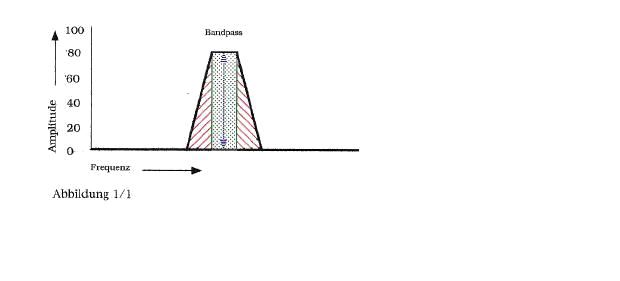
\includegraphics[width=1\textwidth]{images/nono/hph/ab_v_01.jpg}
\caption{}
\label{hph-img1}
\end{center}
\end{figure}

Mentre i due musicisti ed io abbiamo condotto i nostri esperimenti acustici, Luigi Nono deve aver aperto la porta del nostro studio e ascoltato gli esperimenti. All'improvviso entrò inaspettatamente, sorrise e disse: sono arrivato dopo tutto. 
Poi ha annotato i risultati tecnici e sonori e come sono stati creati. Soprattutto Roberto ha dovuto mostrargli il suo nuovo flauto contrabbasso. Nono studiò i singoli campi di tono e suono, mise i suoi appunti nella sua borsa e disse: Devo tornare all'Halden-Hotel e continuare a lavorare. E quello stesso pomeriggio e sera, Luigi Nono ha composto le prime battute per "A Pierre", che ha provato, corretto e perfezionato con i musicisti e i tecnici dello Experimental Studio il giorno successivo. 
Tornato a Venezia Nono finì immediatamente la versione finale di "A PIERRE", la prima esibizione avvenne pochi giorni dopo il 26 marzo 1985 a Baden-Baden, in occasione del 60 ° compleanno di Boulez. 
Quindi, fate la genesi di Luigi Nonos A Pierre. Nono aveva studiato i nostri esperimenti sonori con molta attenzione e integrato nel suo nuovo lavoro in una forma completamente nuova. Il tempo di ritardo 12 e 24 secondi sono stati adottati da lui. Ha fatto uso del fatto che il suono della ripetizione filtrata e poco riverberata è andato ad estendere lo strato dopo 12 secondi. 

\begin{figure}[htbp]
\begin{center}
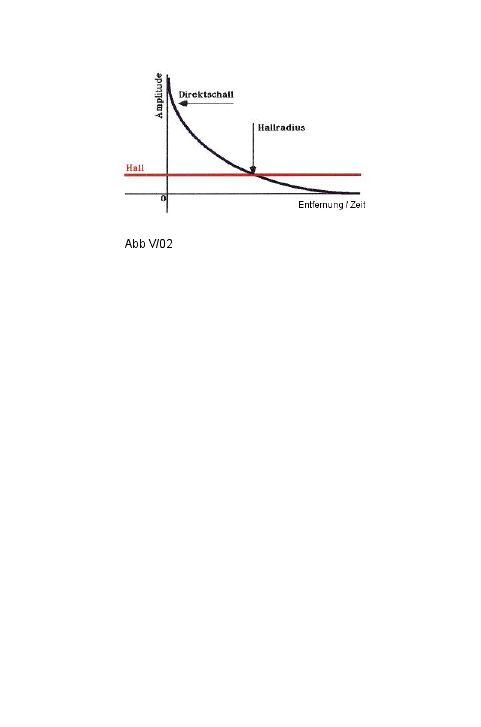
\includegraphics[width=1\textwidth]{images/nono/hph/ab_v_02.jpg}
\caption{}
\label{hph-img2}
\end{center}
\end{figure}

Conosciamo questo processo acustico come eco radiale, immagine 2. Con la diminuzione della dinamica del suono diretto e l'identica intensità del riverbero, percepiamo psicologicamente il suono diretto sempre più diffusamente in una distanza crescente. Questa estensione dello spazio sonoro diventa più chiara dalla trasformazione del suono diretto, dalla selezione del suono. Accanto al suono originale degli strumenti ci sono altri due livelli sonori, che sono enfatizzati dal loro ritardo di 12 e 24 secondi. Questa non è una dinamica, ma come accennato prima, un'estensione dello spazio dell'immagine sonora. 
Nono sapeva dai nostri esperimenti a Friburgo, che questo poteva essere realizzato con un'idea musicale speciale e creato una forma di composizione strettamente orizzontale. 

\begin{figure}[htbp]
\begin{center}
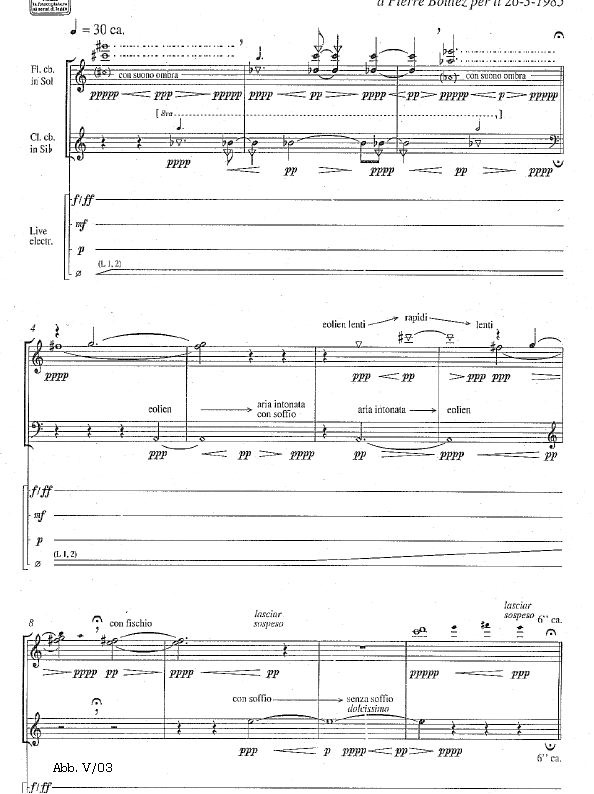
\includegraphics[width=1\textwidth]{images/nono/hph/ab_v_03.jpg}
\caption{}
\label{hph-img3}
\end{center}
\end{figure}


A prima vista, la partitura appare molto semplice, ma chiunque abbia studiato l'eccellente introduzione a A PIERRE nella Ricordi - avrà notato che Nono richiede per quasi ogni nota una forma di interpretazione individuale: dal fischio al fischietto. Per questo motivo, posso raccomandare lo studio di questi testi in tre lingue: italiano, inglese e tedesco. 
Nono crea strutture sonore piene di contrasti che, secondo il tono, variano da suoni e toni pacifici ad aggressivi. Oltre a questo, il compositore ha utilizzato una trasformazione del suono per gli strumenti. Questa trasformazione - un piccolo sept e un tritone più basso - era guidata da un yy slow vibrato, che portava a un controllo variabile del pitch. Al fine di evitare un effetto sirena, questa trasposizione deve essere controllata molto dolcemente. Questa ricchezza di schemi sonori di entrambi gli strumenti suona insieme alla selezione del suono nei filtri passa banda e la trasformazione del suono crea nuovi spettri sonori molto interessanti, che - come mostrato nella figura 3 - possono essere ascoltati nella forma orizzontale di composizione di Nono in tutte le sottigliezze e vari livelli di suoni. 
Certamente, Luigi Nono aveva già utilizzato materiali sonori simili per gli strumenti in "Amendes Klarsein" o in "Prometeo", ma insieme alla legenda tecnica finale come mostrato nel diagramma 4, il compositore realizza un'espressione musicale completamente nuova. 

\begin{figure}[htbp]
\begin{center}
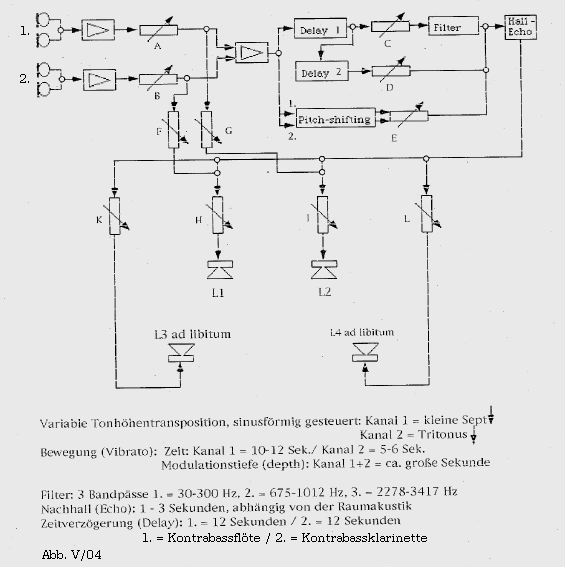
\includegraphics[width=1\textwidth]{images/nono/hph/ab_v_04.jpg}
\caption{}
\label{hph-img4}
\end{center}
\end{figure}

I singoli valori per il controllo dinamico e il tempo di riverbero sono indicati in percentuali relative e devono essere adattati all'acustica individuale della sala da concerto. La dinamica di Nono spazia da 5 pianissimos a forte, dove l'eruzione al forte appare solo una volta. Il più delle volte il volume varia attorno al pianissimo. Nono sviluppò ulteriormente la mia concezione di base dei miei esperimenti per evitare la ripetizione canonica udibile. Sulla base dei fermati a ripetizione continua di circa 6 secondi, la sequenza rigida di ripetizioni di 12 e 24 secondi si dissolve completamente. Così Nono impedisce una periodicità all'interno della sua musica che spesso si rivela molto differenziata e non ritmica, la cui forma interiore è composta in funzione del tempo. Pertanto, la direzione del suono deve essere così trasparente che l'ascoltatore non può verificare ciò che viene riprodotto in origine o ciò che viene riprodotto dagli altoparlanti. Due altoparlanti collocati dietro i solisti sono stati forniti per una performance. Successivamente, Nono collocò due altoparlanti aggiuntivi sul retro dell'auditorium, soprattutto nelle grandi sale da concerto, con la nota esplicita "ad libitum". Inoltre, il volume di questi 2 altoparlanti aggiuntivi 3 e 4 - dopo gli esperimenti con il compositore - deve essere controllato separatamente dagli altoparlanti 1 e 2. Il diagramma 5 mostra la relazione di dinamica tra gli altoparlanti. 

\begin{figure}[htbp]
\begin{center}
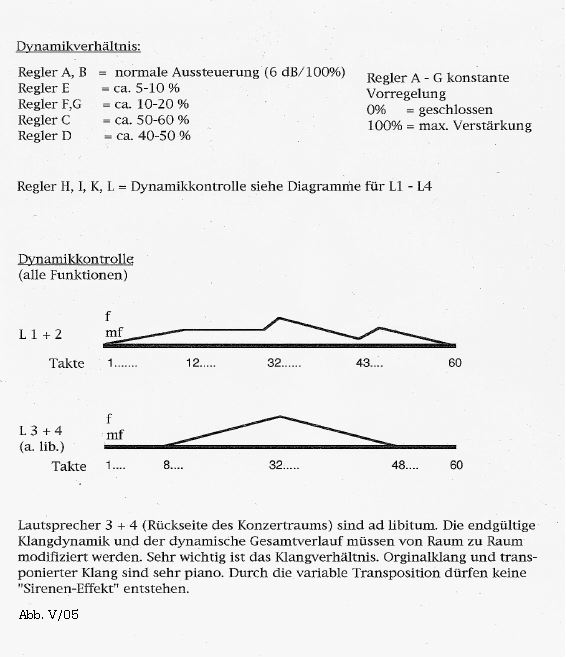
\includegraphics[width=1\textwidth]{images/nono/hph/ab_v_05.jpg}
\caption{}
\label{hph-img5}
\end{center}
\end{figure}

C'è stato il rimprovero che Live-Electronics, la trasformazione elettronica del suono sarebbe attributi di una composizione, che era stata aggiunta dopo il completamento del lavoro. Penso che non ci siano più composizioni tipiche di A Pierre e Omaggio a György Kurtag di Luigi Nono, che sconfiggono totalmente questo rimprovero. In entrambi i lavori, Nono ha incluso nel suo processo compositivo Live-Electronic come materiale equivalente accanto a strumenti meccanici tradizionali o voci. Entrambe le opere perderebbero la loro sostanza musicale senza l'estensione elettronica. 
Lo sperimenteremo soprattutto nella recensione di Omaggio a György Kurtag. Per questo ora ho preparato un piccolo esempio con flauto solo. Innanzitutto, ascolterai un paio di battute da "A Pierre" senza Live-Electronics, quindi la stessa parte con estensione sonora elettronica: 

Gli esempi sonori sono in mono. Il download completo è necessario prima dell'ascolto. 

suono esempio 1 (Martin Fahlenbrock, flauto contrabbasso) 
suono di esempio 2 

Ci sono esempi che mostrano chiaramente che senza la transistor elettronica del suono, l'estensione del suono, uno strumento, manca una parte della sostanza compositiva. Come ho detto prima, dagli esperimenti di Freiburger, Nono sapeva esattamente i risultati sonori delle doppie ripetizioni, originali e trasformati. Ha composto le note degli strumenti con questo risultato, creando così una perfetta armonia tra meccanica e strumento elettronico. Non nego che ci siano composizioni, ad esempio Emmanuel Nunes: "Wandlungen", che può essere eseguita con e senza Live-Electronics. Tuttavia ciò non è possibile con le opere di Nonos create in collaborazione con Experimental Studio. Esigono un equilibrio tra i suoni degli strumenti tradizionali e i suoni della trasformazione elettronica. Di conseguenza non è possibile organizzare né nelle parti strumentali né nelle parti vocali e tecniche senza distruggere il suono che il compositore aveva puntato all'originale. 

Ascoltiamo ora una sezione di "A Pierre" di Luigi Nono in una registrazione subito dopo il completamento della composizione, realizzata nel Freiburg Experimentalstudio (flauto di contrabbasso Roberto Fabbriciani e clarinetto contrabbasso Ciro Scarponi). 

suono di esempio 3 

\section{OMAGGIO A GYÖRGY KURTÁG}

La prima rappresentazione di "Omaggio a György Kurtág" il 10.6.83 a Firenze è stata una delusione per molti ascoltatori. È stata davvero una prima esibizione? 
Nono stava lavorando a "Guai ai gelidi mostri" e "Prometeo" in quell'anno. Molte prove sperimentali hanno avuto luogo con la cantante Susanne Otto, lo strumentista Roberto Fabricciani, Ciro Scarponi e Giancarlo Schiaffini nello studio di Friburgo, una di queste prove è stato il concerto a Firenze. La composizione "Omaggio a György Kurtág" consisteva in valori soglia musicali, che Nono aveva indicato per ogni interprete in tono, spettri sonori e dinamici. Il compositore aveva anche dato alcuni suggerimenti per la tecnica della trasformazione del suono, che, tuttavia, non aveva nulla da fare con la versione finale di "Omaggio". Va detto che Luigi Nono, Alvise Vidolin e io - con la collaborazione dei musicisti - avevamo presentato una introduzione sulla trasformazione del suono elettronico all'inizio del concerto. Vorrei dire che la performance è stata un concerto di lavoro con il titolo: Composizione in corso. Nono non ha tratto profitto da questa esperienza in concerto fino alla sua composizione "Post-Prae-Ludium Donau" del 1987 per tuba solo e live-electronics. In questa composizione, per il musicista, valori di soglia, altezza, spettro sonoro, strutture ritmiche, scale di toni, volume e, soprattutto, sono state definite le strutture temporali. Gli intervalli devono essere riempiti dall'interprete mediante improvvisazioni. Sono indicati funzioni sonore e programmi per l'elettronica. 
Quello che sto per dire ora si riferisce esclusivamente alla versione di "Omaggio", che è stata eseguita per la prima volta a Torino, il 6 giugno 1986. 
All'inizio della mia conferenza scrissi: composizioni, in cui Luigi Nono aveva integrato in modo stringente una funzione estesa del tempo. Per A Pierre, Nono applica un ritardo di segnali acustici nel tempo, ripetizioni senza feedback. Sebbene questi determinino formalmente la composizione, l'idea di base di "Omaggio a György Kurtag" era completamente diversa. 
Nono mi aveva comunicato il suo primo schizzo in una lettera: 

\begin{figure}[htbp]
\begin{center}
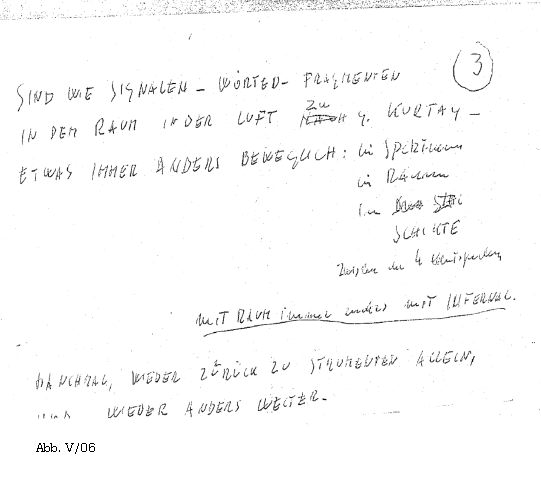
\includegraphics[width=1\textwidth]{images/nono/hph/ab_v_06.jpg}
\caption{}
\label{hph-img6}
\end{center}
\end{figure}

Cosa significa questo? 
1.) La musica dovrebbe essere come segnali, parole, frammenti nell'aria, in 
spazio a György Kurtag. 
2.) Riguardo l'uso della trasformazione del suono elettronico Nono scrive: 
Sempre nuovo, mai rigido, ma 
cambio dello spettro, filtro passa banda, 
cambiamento del suono dello spazio, varie posizioni del suono (4 altoparlanti), movimenti del suono, (esteso a 6 altoparlanti durante le prove), 
La modifica del feedback significa feedback diverso al ritardo dei segnali. 
3:) A volte solo strumenti, nient'altro che il suono strumentale e vocale originale. 
4.) E ancora con live-electronics. 
Per capire meglio, daremo un'occhiata alla foto 7, la leggenda tecnica, che ho registrato in questa forma durante le prove a Torino. 

\begin{figure}[htbp]
\begin{center}
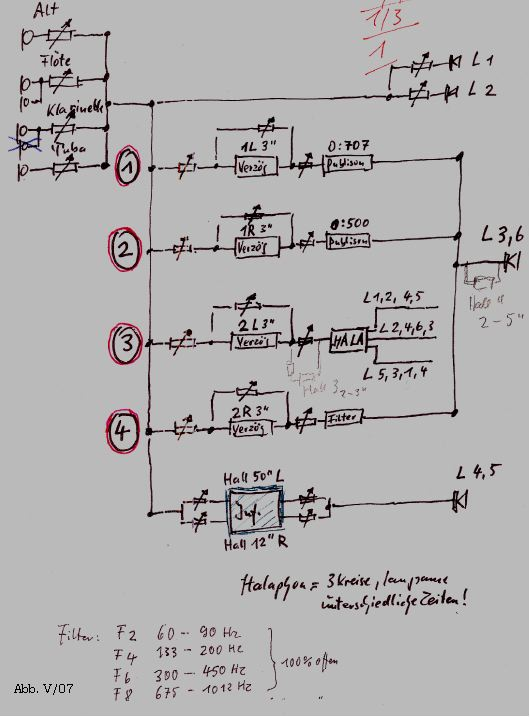
\includegraphics[width=1\textwidth]{images/nono/hph/ab_v_07.jpg}
\caption{}
\label{hph-img7}
\end{center}
\end{figure}

Per evitare equivoci, ho chiamato i programmi con combinazioni. Tutti e quattro sono ritardati di 3 secondi, con e senza feedback. A seconda della dinamica del feedback, i segnali di ingresso degli strumenti e la voce si attenuano in modo diverso. Al massimo una miscela di suoni nell'apparecchiatura di ritardo può essere memorizzata acusticamente per un periodo di tempo più lungo, alimentando le scale parzialmente orizzontali dei suoni originali sovrapposti, compressi e trasformati in una struttura verticale del suono. Nella sua lettera, Nono lo chiama: cambiamento nel feedback, che significa volume di feedback. Il cambiamento dello spettro sonoro - Nono non solo può ascoltarli durante le prove, ma anche vederli tridimensionalmente su uno schermo e battere con precisione - queste mutazioni sonore sono ottenute da tre possibilità: 

1.) suddivisione dello spettro sonoro nei suoi singoli toni parziali. Conosciamo queste selezioni dalla prima ripetizione su A Pierre. 
2.) Trasposizione di spettro in un harmonizer. Per "Omaggio" Nono ha scelto la trasposizione di un tritone e un'ottava più in basso. Mescolato con il suono originale, viene creato un nuovo spettro sonoro, dipendente dal volume di trasposizione. 

Da un lato, lo spazio sonoro è cambiato da varie classi con i segnali di uscita ai 6 altoparlanti, dall'altro un movimento sonoro '150; ricorda alla combinazione tre. I movimenti sonori sono realizzati in tre diverse direzioni di movimento lente con un'apparecchiatura di controllo dello spazio sonoro universale, l'halaphone e sono definiti con precisione dal compositore. I singoli movimenti di direzione sono controllati tramite altoparlanti. 
Fin dall'inizio, Luigi Nono ha avuto un'idea molto precisa dell'uso della trasformazione del suono elettronico per la sua composizione, che poi è stata resa più precisa durante le prove, Confrontiamo ancora una volta le figure 7 e 6. 

Immagine 6 

Immagine 7 

Spectre - combinazione 4 , 5 filtri passa banda 

spettro - combinazione 1 e 2 , trasformazione del suono 

Combinazione 3- spazio - classificazione di altoparlanti, movimento del suono 
Riverbero (12 + 50 secondi) 

Feedback: ritardo di tre secondi con vari feedback 

Corrispondente al suo schizzo tecnico, Nono ha composto la voce e la partitura strumentale: 

Contrariamente a una forma prevalentemente verticale di Pierre, soprattutto alla realizzazione del lungo riverbero e dei suoni compressi dal feedback. 

\begin{figure}[htbp]
\begin{center}
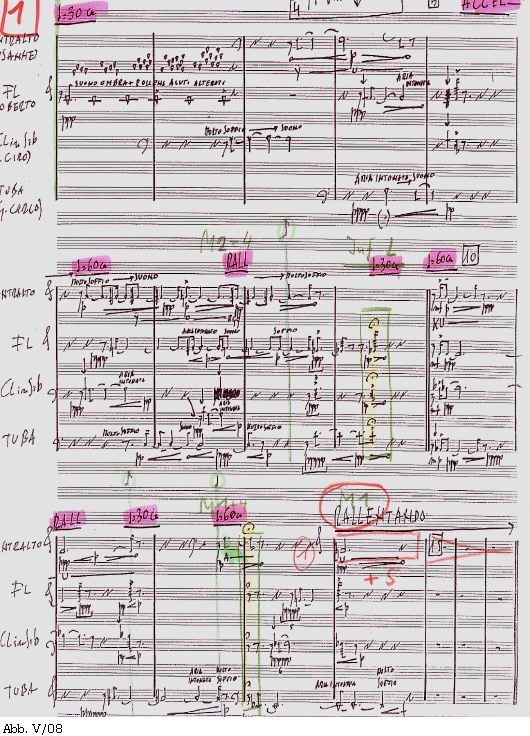
\includegraphics[width=1\textwidth]{images/nono/hph/ab_v_08.jpg}
\caption{}
\label{hph-img8}
\end{center}
\end{figure}

Nella figura 8 vediamo la prima pagina della partitura scritta a mano con note supplementari di controllo del suono, prima esecuzione, Torino. Nella barra 9, contrassegnata in verde, l'accordo dello strumento di ottone viene riverberato artificialmente per 50 secondi. Naturalmente, l'intensità di questo accordo - pianissimo - accorcia molto il riverbero. La durata del riverbero dipende dall'intensità del segnale di ingresso. Pertanto, Nono non indica una durata esatta, ma collega questo riverbero tecnicamente inesatto da un arresto. Ma ciò che può essere ascoltato, tuttavia, è il volume del suono, che corrisponde alla dimensione di una stanza geometrica di 50 secondi. Pertanto è importante che vengano utilizzate solo apparecchiature di ritardo con un volume di spazio controllato. La suddetta fermata consente al controllo del suono di variare in modo variabile attenuando il tempo di riverbero in base alle dimensioni della sala da concerto. Gli intervalli sonori realizzano lo schizzo di Nono. "come segnali a György Kurtag" Dove troviamo un intervallo sonoro più breve nella battuta 13, Nono impiega la prima versione di un intervallo sonoro di delay con feedback per il contralto nella barra da 14 a 17. Il tempo prescritto è un quarto di nota uguale a 60 , il tempo di ritardo con feed-back di 3 secondi. Con una mezza nota del contralto, si ottiene una ripetizione con un semplice feedback. La funzione di fadeout altrettanto breve del feedback è contrassegnata in rosso. Il suono originale della voce viene trasposto nel delay di un tritone in basso (combinazione 1). 

\begin{figure}[htbp]
\begin{center}
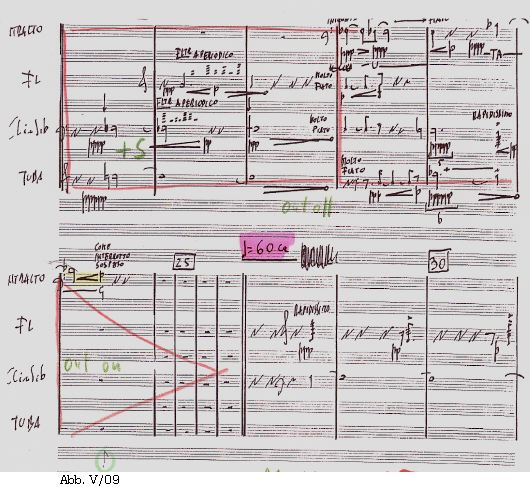
\includegraphics[width=1\textwidth]{images/nono/hph/ab_v_09.jpg}
\caption{}
\label{hph-img9}
\end{center}
\end{figure}

Nelle barre 18-20, Nono impiega la seconda versione dell'intervallo sonoro per ritardo con feedback. Tuttavia, vista formalmente, questa versione è completamente cambiata rispetto alla battuta 14. Il suono originale degli strumenti di ottone viene di nuovo ritardato di tre secondi con un feedback e una trasposizione di un tritone più in basso. Il risultato non può essere ascoltato immediatamente, ma viene riprodotto nella battuta 23 -27. Questo effetto acustico può essere chiamato eco con una lunga riverberazione, ovvero l'intensificazione del suono della barra 18-20 può essere percepita solo 20 secondi dopo. Un'idea compositiva, che combina due funzioni temporali in un unico complesso: durata della ripetizione con feedback e durata dell'eco. Nell'esempio 4, prima ascolteremo lo spazio sonoro ingrandito e il riverbero sovradimensionato. 

suono di esempio 4 

Il feedback è stato sbiadito. Nell'esempio seguente, ascolteremo un ritardo con feedback, formiamo uno senza cambiamenti nel tempo. Vorrei richiamare la tua attenzione sulla trasposizione in un tritone più in basso. 

suono di esempio 5 

La terza versione, il suono originale compresso e trasposto con riproduzione indietro spostato nel tempo. Il feedback si attenua lentamente, c'è un naturale sbiadimento dovuto alla dissoluzione della densità del suono. Questa procedura tecnica è particolarmente importante per una performance. 

esempio sonoro 6 

Questi esempi sonori sono continuamente modificati - come sappiamo dalla leggenda tecnica - durante l'intero lavoro. Così il compositore realizza il suo concetto: "Qualcosa è continuamente e diversamente flessibile" 

La restante parte di voce e strumento rimane invariata senza la trasformazione del suono. Con questo, Luigi Nono enfatizza la funzione di live-electronic, gli intervalli sonori creano nuove dimensioni del suono e del tempo. Citazione del compositore: nello spazio cosmico verso l'universo, altri spazi, altre terre, altri abissi, altre fantasie. (Fine della citazione). 
Con questi due lavori, "A Pierre" e "Omaggio a György Kurtág", Luigi Nono ha scoperto nuovi strati sonori, che ha potuto realizzare con l'aiuto della tecnica moderna, la trasformazione elettronica del suono. Sebbene diversi negli strumenti, diversi nella forma della composizione, entrambe le opere hanno un significato comune, un concetto spirituale comune. 

Ascoltiamo "Omaggio a György Kurtag" due volte. Durante il primo replay, ti mostrerò il punteggio sullo schermo, per dimostrare cosa intendevo mostrare. prima. Poi ascolteremo il breve brano, circa 15 minuti, ascolteremo la musica di Nono, senza essere distratti dalle impressioni visive. Quest'opera di Nono è stata pubblicata in un'ottima edizione dalla casa editrice Ricordi. Sto usando una copia della partitura originale, poiché ho usato i colori per tutte le funzioni di live-electronic durante le prove per la prima esibizione a Torino. 

Esempio 7 (con schermo) 
Esempio 8 (senza schermo) Si prega di ascoltare gli esempi 7 e 8 dal CD "luigi nono 3", AUVIDIS FRANCE, MO 782047.

% !TEX encoding = UTF-8 Unicode
% !TEX TS-program = pdflatex
% !BIB program = biber
% !TEX root = ../../2017-GS-COME01-INVITO-ASCOLTO.tex

%\input{../../_template/latextemplate/gs_article_style_01.tex}

%----------------------------------------------------------------------------------------
%	TITLE SECTION
%----------------------------------------------------------------------------------------

%\usepackage{fancyhdr} % Headers and footers
%\pagestyle{fancy} % All pages have headers and footers
%\fancyhead{} % Blank out the default header
%\fancyfoot{} % Blank out the default footer
%\fancyhead[C]{analisi di DIALOGUE DE L'OMBRE DOUBLE di Pierre Boulez  $\bullet$ Giuseppe Silvi }%$\bullet$ Vol. XXI, No. 1} % Custom header text
%\fancyfoot[RO,LE]{\thepage} % Custom footer text
%
%\title{\vspace{-15mm}\fontsize{24pt}{10pt}\selectfont\textbf{analisi di\\ \smallskip \emph{DIALOGUE DE L'OMBRE DOUBLE}\\ \smallskip di Pierre Boulez \\ [1.5em]}} % Article title
%
%\author{
%\large
%%\textsf{Storia e analisi del repertorio della musica elettronica ed elettroacustica I} \\[.7em]
%\textsf{Dipartimento di Nuove Tecnologie e Linguaggi Musicali} \\
%\textsf{Conservatorio di Musica S. Cecilia di Roma} \\[.7em]
%\textsc{\textbf{Giuseppe SILVI}} \thanks{Ringraziamento speciale al Mº Nicola Bernardini per la fornitura della partitura originale e di preziosi appunti d'esecuzione; a Sara Ferrandino per la traduzione del documento video \emph{Dialogue de l'ombre double de Pierre Boulez; un dialogue avec Jérôme Comte et Alain Damiens.}}\\ %[5mm] % Your name
%\normalsize grammaton [at] me [dot] com \\ % Your email address
%\vspace{-2em}
%}
%\date{{\small \today}}
%
%%----------------------------------------------------------------------------------------
%
%\begin{document}
%
%\hyphenation{cla-ri-net-to}
%
%\maketitle % Insert title
%
%\thispagestyle{empty} % All pages have headers and footers

%----------------------------------------------------------------------------------------
%	ARTICLE CONTENTS
%----------------------------------------------------------------------------------------

\clearpage

\thispagestyle{empty}

\includepdf[scale=1.03,
		    pagecommand={
		    	\begin{tikzpicture}[
					remember picture,
					overlay]
		    	\node [xshift=2cm,yshift=1cm] at (current page.south west) {\color{white}{\emph{Heinz \textbf{Karnine}}}};
				\end{tikzpicture}}
		    ]{images/stockhausen/stockhausen.pdf}

\clearpage

%-------------------------------------------------------------
%---------------------- LUIGI NONO - OMAGGIO A GYORGY KURTAG -
%-------------------------------------------------------------

\chapter*{1985. Pierre Boulez.\\\emph{Dialogue de l'ombre double}.}
\addcontentsline{toc}{chapter}{1985. Pierre Boulez. \emph{Dialogue de l'ombre double}.}

\section*{Scheda dell'opera}

\begin{table}[ht]
%\caption{default}
\begin{center}
\begin{tabular}{>{\sffamily}r>{\normalsize }p{7.5cm}}

\hline
\hline
											& \\
autore:										& Pierre Boulez (1925) \\
titolo:										& \textbf{Dialogue de l'ombre double} \\
											& \textsf{per clarinetto/primo sul palco} \\
											& \textsf{e clarinetto/doppio registrato} \\
											& \\											
dedica:										& \emph{A Luciano Berio per il suo sessantesimo compleanno} \\
data di composizione:						& 1984-85 \\
durata:										& 20' \\
											%& \\
Editore:									& Universal Edition \\
Codice di catalogo							& UE 18407 \\
produzione elettronica:						& IRCAM, Parigi \\
realizzazione:								& Andrew Gerzso \\
dispositivi:								& Suono su supporto \\
											%& \\
prima Esecuzione:							& Alain Damiens, 28 Ottobre 1985, Firenze \\
											& \\
\hline
\hline

\end{tabular}
\end{center}
%\label{default}
\end{table}%

%----------------------------------------------------------------------------------------
%	BEGIN MULTICOLS
%----------------------------------------------------------------------------------------

%\begin{multicols}{2} % Two-column layout throughout the main article text

\section*{Introduzione}

%\begin{description}
%{\small
%\item[Dialogo] - \textgreek{διάλογος}, da \textgreek{διαλέγομαι} “converso”.}
%\end{description}

Il \emph{Dialogue de l'ombre double}, composto e dedicato a Luciano Berio nel 1985, rappresenta, per diversi motivi, un brano di particolare interesse nel repertorio della musica elettroacustica. È un brano che si avvale del supporto elettronico per la sola registrazione del clarinetto/doppio, ma richiede una messa in scena sonora articolata nella diffusione in sala mediante una complessa regia del suono. Il brano, prodotto all'interno dell'IRCAM si avvale delle conoscenze e delle tecniche sviluppate intorno al live electronics, nel contesto di speculazione sullo spazio sonoro da cui è nato poco prima anche \emph{Répons}.%\footnote{\emph{Répons, per sei solisti, orchestra da camera e live electonics}}.

\clearpage

%%------------------------------------------------- IMMAGINE
%
%\begin{figure}[H]
%\begin{center}
%\includegraphics[width=.47\textwidth]{img/ED01_tetrarec_lucier13degrees_CG.jpg}
%\caption{Dettaglio della disposizione dei microfoni durante la registrazione Tetraedrica Spaziata. }
%\label{default}
%\end{center}
%\end{figure}
%
%%------------------------------------------------- IMMAGINE

\begin{flushright}
{\small
\textit{ 
L'ordine è il piacere della ragione:\\ma il disordine\\ è la delizia dell'immaginazione.\\ Però i calzini usati mettili in lavatrice.\\
 }\textbf{Paul Claudel}}%, La scarpina di raso}
\end{flushright}

%Quote rosso1 Il segreto della creatività è il saper nascondere le proprie fonti. Quote rosso2 
%~ Albert Einstein

\section*{Strutture}

%Dialogo doppia ombra, dedicato a Luciano Berio e scritto per il suo sessantesimo anniversario nel 1985, è stato creato 28 Ottobre 1985 a Firenze da Alain Damiens. Il lavoro viene svolto presso l'IRCAM di Andrew Gerzo, assistente musicale. Su suggerimento di Pascal Gallois, Pierre Boulez nel 1995 trascritto per fagotto, che aveva fatto in precedenza per i campi, un altro dei suoi lavori per clarinetto. In dialogo, la musica rimane la stessa, ma i diversi registri di entrambi gli strumenti richiedono trasposizioni.

Tra il 1946 e il 1958 Pierre Boulez fu direttore musicale della compagnia teatrale \emph{Renaud-Barrault}. In quel contesto incontrò Paul Claudel. \emph{L’ombra doppia} è il titolo di una scena della \emph{Scarpina di raso} di Claudel alla quale il \emph{Dialogue de l'ombre double} è ispirato, dove un gioco di luci proietta una doppia ombra sullo sfondo della scena. Qui, nell'opera di Boulez, è il clarinetto a sdoppiarsi in un intreccio dialogico tra le due parti.

\begin{quote}
{\small
\textbf{Dialogo} - La parte di uno scritto e, più spesso, di un’opera scenica, narrativa, o di un film, in cui sono introdotti a parlare due o più personaggi. -- \textbf{letteratura} Prescindendo dalle opere sceniche, dove è nel suo proprio luogo, e senza tener conto degli elementi dialogici contenuti nelle liriche, nei poemi, nella prosa narrativa, il d. come genere letterario si può dire nasca con Platone, per l’esigenza di presentare drammaticamente il processo di scoprimento e di conquista della verità, attraverso il contrasto di opposte opinioni. [\ldots] -- \textbf{musica} Composizione vocale (per due o più voci accompagnate) del 16º-17º sec., su testo religioso o profano, in forme dialogica. Il termine indicava anche un componimento per due o più strumenti, in stile concertante, in forme varie, coltivato nel 17º secolo.\footnote{http://www.treccani.it/enciclopedia/dialogo/}}
\end{quote}

La forma del dialogo si sviluppa tra il \emph{clarinette/première} e \emph{clarinette/double} nell'alternanza di \emph{strophe} (il primo) e \emph{transition} (il secondo). Entrambe sono eseguite dallo stesso musicista: il discorso si svolge dal vivo tra il clarinetto sul palco e il suo doppio pre-registrato e diffuso dagli altoparlanti. Alla presenza localizzata del primo, si oppone l'immagine diffusa dell'altra. Nello sviluppo dialogico, le strofe sono focalizzate su singole idee compositive mentre le transizioni si spostano gradualmente da un modello ad un altro.

Non c'è sovrapposizione tra l'esecuzione dal vivo ed il nastro pre-registrato, tranne nei periodi di passaggio, ma  senza creare polifonia, in un gioco di ombre che si succedono proseguendo la dimensione orizzontale del testo del discorso. Ora, un vero dialogo tra due soggetti comporta un corso irreversibile del tempo, mentre nella duplicazione della personalità lo sviluppo temporale, come in una riflessione interiore, il tempo non è lineare ma circolare. Formalmente il sistema è reso ancora più ampio e multi-direzionale dalla forma a due percorsi, identificati rispettivamente con numeri arabi o numeri romani.

%Acronimo finale: l'ombra sussurrò alterna passaggi (full circle) e improvvise interiezioni. Dal momento che il suono iniziale, prima filtrato si sviluppa a poco a poco ad essere trasmesso da tutti e tre gli altoparlanti alti.

In ciascuno dei percorsi l'alternanza tra strumento e ombra sviluppa il discorso musicale, a volte condiviso a volte smembrato fino alla fine, trovandosi d'accordo in un unisono.

Nella stesura formale del brano, il doppio, lo sdoppiamento, si gioca anche sul piano della scelta: l'esecutore può scegliere due percorsi tra strofe e transizioni, indicati il primo con \emph{cifre romane} ed il secondo con \emph{cifre arabe}. %La \emph{Sigla iniziale} e la \emph{Sigla finale} sono comuni ad entrambi

\thispagestyle{fancy} % All pages have headers and footers

\section*{Sigla Iniziale}

Entrambe le sigle sono suonate dal \emph{clarinetto/doppio}. La \emph{Sigla iniziale} è giocata interamente sull'articolazione della terzina come nocciolo dell'incedere cellulare. Cardine di questi brevi sviluppi è il \emph{Re3}\footnote{Espresso in suoni reali, un tono sotto alla notazione in partitura \emph{Mi3}} sul quale Boulez sospende ogni periodo, chiudendo le legature e posizionando la sorgente in punti doversi dello spazio. In un gioco di doppi, un omaggio a Berio non si può ritenere concluso senza intricare il racconto con riferimenti intarsiati nel discorso musicale. A sottolineare il legame tra i due compositori ci sono numerosi riferimenti. Uno di questi è proprio il \emph{Re3}, nota polarizzante sia dell'inizio che della fine della \emph{Sequenza IXa} di Berio.
Volendo indugiare nella ricerca di riferimenti, la stessa figura iniziale della terzina è cardinale nel rigo iniziale della \emph{Sequenza}. 

L'intero progetto delle \emph{Sequenze} di Berio descrive accuratamente il tentativo di spingere la pratica strumentale verso un'evoluzione si tecnica ma anche mentale, di approccio e ricerca con lo strumentista ed il suo strumento tradizionale. In un modo simile l'amico Boulez sfruttò il rapporto con Alain Damiens, clarinetto dell'Ensemble Inter-Contemporain, impostando il lavoro

\begin{quote}
{\small
in modo molto didattico, spingendo l'interprete fino ai limiti, affinché egli stesso ne verifichi le possibilità.
}
\end{quote}

%%%%%%%%%%%%%%%%%%%%%%%%%%%%%%%%%%%%%%%%%%%%%%%%%%
% STROFE
%%%%%%%%%%%%%%%%%%%%%%%%%%%%%%%%%%%%%%%%%%%%%%%%%%

\section*{Strofe}

La partitura comprende quindi sei strofe ordinate in modo diverso nel caso che si scelga la numerazione romana o araba. 

\begin{minipage}[t]{0.89\columnwidth}%

\begin{table}[H]
%\caption{default}
%\begin{center}
\begin{tabular}{c c c}

I 	& = & 2 \\
II	& = & 4 \\
III	& = & 1 \\
IV	& = & 6 \\
V	& = & 3 \\
VI	& = & 5 \\

\end{tabular}
%\end{center}
%\label{default}
\end{table}%

\end{minipage}%
\bigskip

La \emph{Strofa I(2)} si basa su un processo di scrittura che verrà ampiamente sviluppata durante il lavoro. %Clarinetto Monody è una giustapposizione di cellule alla maniera di un filo di perle. Queste cellule sono polarizzati (+/-), vale a dire che sono fatte da alci e finali (tempo / venduto). Le cellule regolarmente si alternano a cellule mezzo piano Mezzo Forte.

La \emph{Strofa II (4)} inizia in modo molto dolce, quando uno shock nervoso, un'eruzione vulcanica, appena traumatizzare il discorso. Queste pause appaiono sporadicamente, meno prominente. Tra questi, troviamo la sequenza di celle con valori ritmici meno tesa.

La \emph{Strofa III(1)} gioco di scrittura tra fili di suoni, tenuta e attacchi con terminazioni sforzando fuggitive.

La \emph{Strofa IV(6)} la scrittura, tritato sciolsero, opponendosi alla grande aumento nella quinta strofa.

La \emph{Strofa V(3)} la sequenza porta ad un clima nella parte centrale, dove le cellule sono notevolmente allungati nel tempo e suono, esaltata dalla riverberazione del pianoforte e diffusione di altoparlanti. Alla fine di questa stanza, le cellule riprendono le normali proporzioni e riverbero diminuisce.

La \emph{Strofa VI (5)} è la liberazione. Questa stanza si sviluppa alta vocalizzo, estensione vocale flessibile su una raffica. Le oscillazioni di tempo, in fuga instabile. Questa frase culmina verso acuto e stridente tenuta prima di cadere nella seconda parte del versetto, nel registro inferiore ancorato D, porto di partenza del clarinetto in questo pezzo. Fraseggio alterna linea continua e ornamenti flatterzunge.

\section*{Transizioni}

Attraverso il racconto di Alain Damiens si può ricostruire come l'idea stessa di evoluzione dialogica del brano sia passata negli anni attraverso più fasi compositive.

\begin{quote}
{\small
Il \emph{Dialogue}, nella storia del compositore, deriva da un brano che si chiama \emph{Domaines} che compose nel 1967, quando era professore di composizione al conservatorio. Chiese per esercizio agli allievi di comporre un pezzo per un strumento solista, deliberatamente asettico, con una simbologia numerica. Un brano contemporaneamente aperto e chiuso. In tutto questo si mise lui stesso ad eseguire l'esercizio e ne ricavò una piccola raccolta, il quaderno A, un “domaine” di circa 40 secondi. Poi sviluppò l'idea in 12 raccolte, 6 originali e 6 speculari e poi compose i \emph{Domaines} per gruppi di strumenti sempre da 1 a 6. Poi cambiò di nuovo idea e riscrisse tutto. Prese la prima raccolta ed i sei moduli per ensemble e sviluppò tutto per doppio clarinetto, elaborando la logica con cui in \emph{Domaines} faceva dialogare il solista con il gruppo. Il tutto passando dai 40 secondi iniziali ai 18 minuti.
}
\end{quote}

Il processo di sviluppo graduale del brano riguarda anche l'introduzione dell'elettronica, in quanto 
\begin{quote}
{\small
all'inizio prospettava due persone fisiche sulla scena ma questo poneva molti problemi tecnici e quindi ha optato per la registrazione: si suona sul proprio suono.
}
\end{quote}

In termini pratici, il racconto di Damiens ci fornisce i numeri per capire perché le strofe sono identiche per entrambi i percorsi (romano, arabo) ma con ordine diverso, mentre per le transizioni si hanno quattro identità e due particolarità:

\begin{minipage}[t]{0.89\columnwidth}%

\begin{table}[H]
%\caption{default}
%\begin{center}
\begin{tabular}{c c c}

I a II 		& = & 2 a 3 \\
II a III	& = & 4 a 5 \\
III a IV	& = & 1 a 2 \\
IV a V		& = &  \\
V a VI		& = & 3 a 4\\
			& = & 5 a 6 \\

\end{tabular}
%\end{center}
%\label{default}
\end{table}%

\end{minipage}%
\bigskip

Il numero delle transizioni è uguale al numero delle strofe meno uno quindi per ognuno dei due percorsi B. necessitava di cinque transizioni mentre, almeno secondo la testimonianza di Damiens, il processo compositivo di B. forniva blocchi di sei oggetti musicali, esattamente quelli che si hanno se si contano le righe della nostra tabella. 

\section*{Sigla Finale}

Come accade per la \emph{Sigla Iniziale}, anche nella \emph{Sigla Finale} l'ombra, il \emph{clarinetto/doppio}, inizia il suo discorso mormorando frasi in \emph{\textbf{pp}} nella gamma inferiore dello strumento, con improvvise  interpunzioni in \emph{\textbf{ff}} e progressive aperture nel registro acuto. Il tutto avviene in un crescendo dato dall'entrata progressiva di diffusori per poi scendere di nuovo all'inverso, in un processo di graduale chiusura di ciascun altoparlante fino alla fine del brano. Il \emph{clarinetto/primo} inizia a suonare un \emph{Do6} pianissimo  nel momento in cui tutti i diffusori sono aperti e lo porta fino alla fine del brano dove incontra il \emph{doppio} che tocca la stessa nota ma viene diffuso nell'altoparlante esterno al cerchio dei sei, quello dedicato all'effetto di distanza. L'ultimo contatto tra i due quindi segna l'allontanamento dell'ombra sullo stesso suono, ad indicareche c'è ancora un ultimo gesto da compiere, ma non è dialogico bensì teatrale: una uscita di scena, una uscita dallo spazio.


%\section{Citazioni}



\begin{quote}
{\small
[\ldots] si ha la sensazione che si riduca enormemente, con una sensazione di claustrofobia e poi si allarghi e si riempia. C'è un bel rapporto tra il pubblico e l'esecutore, molto differente ma entrambi completamente dentro, immersi, non soltanto assorbiti dalla musica ma anche dalla visione teatrale scenica e poi questa ultima posa di suono finale, questa nota che va tenuta indefinitamente davanti al pubblico, concetto incomprensibile di infinito, la musica continua verso la fine.
}
\end{quote}

\section*{Spazio Sonoro}

La spazializzazione del nastro pre-registrato può essere eseguita sia manualmente che in maniera automatizzata. Per al procedura automatizzata si può utilizzare il timecode presente sul secondo canale del tape. 

Le istruzioni per la spazializzazione tra metodo manuale e automatizzato sono minimamente diversificate, in modo che l'esecuzione automatizzata possa eseguire virtuosismi che manualmente sarebbero impossibili o estremamente complessi.

%----------------------------------------------------------------------------------------
%	INTRODUZIONE
%----------------------------------------------------------------------------------------

\section{dalle note tecniche, Introduzione}

Dialogue è una composizione per clarinetto dal vivo (\emph{premiere}) e clarinetto pre-registrato (\emph{double}). Il brano inizia con una sezione di \emph{tape} (\emph{Sigle Initial}) e poi prosegue in un'alternarsi di sezioni dal vivo (\emph{strophes}) e sezioni pre-registrate (\emph{transitions}) per concludere con una sezione di \emph{tape} (\emph{Sigle Final}).

Idealmente l'esecutore si dovrebbe posizionare al centro della sala, circondato dal pubblico. Attorno al pubblico è disposto un cerchio di sei altoparlanti attraverso il quale è riprodotto il \emph{tape} con lo strumento pre-registrato.

FIG 1a

Se non fosse possibile posizionare l'esecutore al centro della sala, si può procedere con il posizionamento tradizionale sul palcoscenico.

FIG 1b

Per ottenere un contrasto maggiore tra le sezioni dal vivo e quelle pre-registrate è necessario utilizzare un'illuminazione dedicata all'esecutore durante le \emph{Strophes}.

Il \emph{tape} dovrebbe essere pre-registrato dallo stesso esecutore. Esiste comunque una versione disponibile presso l'IRCAM.

La composizione è disponibile in due versioni chiamate rispettivamente \emph{Version aux chiffres romains} e \emph{Version aux chiffres arabes}

%----------------------------------------------------------------------------------------
%	STROPHES
%----------------------------------------------------------------------------------------

Durante le \emph{Strophes} il clarinetto dal vivo può essere amplificato attraverso un sistema composto da un microfono e due altoparlanti posizionati accanto al musicista. Nel caso di un'acustica troppo asciutta, lo strumento può essere leggermente riverberato. Durante le \emph{Strophes II, III, V} della versione \emph{aux chiffres romains} e le \emph{Strophes 1, 3, 4} della versione \emph{aux chiffres arabes}, il suono del clarinetto dal vivo è trasformato attraverso un pianoforte nel quale il pedale destro è tenuto abbassato così che le corde possano vibrare liberamente. 

FIG 2

%----------------------------------------------------------------------------------------
%	TRANSITIONS
%----------------------------------------------------------------------------------------

La registrazione monofonica utilizzata per le \emph{transitions} viene riprodotta attraverso sei altoparlanti equidistanti tra loro (1--6) che circondano il pubblico e un altoparlante fuori dal cerchio (7).

\begin{quote}
{\small
Questo ultimo altoparlante, utilizzato solo alla fine della \emph{Sigle Final}, deve suonare essere distante e può essere anche posizionato fuori dalla sala da concerto.


Seguendo i punti di riferimento scritti in partitura, il clarinetto pre-registrato viene inviato tra un altoparlante e un altro dando all'ascoltatore l'impressione che il suono si muova nello spazio fisico. 

D'ora ci riferiremo a questo col termine di “spazializzazione”
}

\end{quote}

Nel \emph{Dialogue} esistono due tipi di spazializzazione:

\begin{description}
\item[continuo] il suono si muove morbidamente tra gli altoparlanti
\item[discreto] il suono si muove bruscamente da un altoparlante all'altro
\end{description}

La spazializzazione può avvenire in due modi:

\begin{description}
\item[manualmente] il livello di ogni altoparlante è controllabile individualmente dai potenziometri di una piccola superficie di mixaggio
\item[automatizzata] la seconda traccia del \emph{tape} può contenere un \emph{timecode SMPTE} inviabile ad un decoder che controlli un sistema automatico in sincronismo con i riferimenti in partitura.

\end{description}

FIG 3

Confrontando le istruzioni manuali e automatizzate per la spazializzazione si può notare che sono praticamente le stesse (anche se spesso annotate in modi leggermente diversi) per quasi tutte le transizioni, fatta eccezione della \emph{Sigle Initial} (sia per la versione \emph{aux chiffres romains} che per la \emph{aux chiffres arabes} -- vedi tabella \ref{tab:diffsiginit}) e della \emph{Transition de IV à V} (quindi solo per la versione \emph{aux chiffres romains} -- vedi tabella \ref{tab:diffiv-v}). Nella \emph{Transition de IV à V} si hanno due procedure di spazializzazione diversificate, una più semplice realizzabile manualmente, una più complessa e virtuosistica automatizzata.

Le indicazioni dinamiche per gli altoparlanti vengono fornite in termini musicali: quando un altoparlante è acceso deve suonare tra il \emph{mezzoforte} e il \emph{forte}. Nella \emph{Transition de I à II} per esempio gli altoparlanti vengono modulati due volte consecutivamente, prima in \emph{forte} poi in \emph{mezzo-piano}. Questi due differenti livelli dinamici vengono determinati in prova e devono descrivere un chiaro effetto di gioco tra primo piano e sfondo. I tempi di crescita verso il \emph{forte} “il più veloce possibile”, mentre il decadimento al \emph{mezzo-piano} deve durare $ 0.5 sec $. Anche le indicazioni di modulazione tra un valore dinamico e l'altro sono espresse nei termini musicali di \emph{crescendo} e \emph{diminuendo}.




\begin{table*}[h]

\caption{confronto tra spazializzazione manuale ed automatizzata SIGLE INITIAL, uguale sia per le cifre romane che per le cifre arabe}
\begin{center}
%\begin{sf}{\footnotesize
\begin{tabular}{c c c c c}

\hline
\multicolumn{5}{c}{\emph{\textbf{Sigle Initial}}} \\
\hline

	&
\multicolumn{2}{c}{\textbf{Spazializzazione Manuale}} &
\multicolumn{2}{c}{\textbf{Spazializzazione Automatica}} \\

\hline

\textbf{cue number} 	& \textbf{speaker(s) ON}	& \textbf{speaker(s) OFF} 		& \textbf{speaker(s) ON} 		& \textbf{speaker(s) OFF} 		\\
1			&	1			&	-					&	1					&	2, 3, 4, 5, 6 		\\
2			&	3			&	1					&	3					&	1, 2, 4, 5, 6 		\\
3			&	5			&	3					&	5					&	1, 2, 3, 4, 6 		\\
4			&	2			&	5					&	2					&	1, 3, 4, 5, 6 		\\
5			&	5			&	2					&	5					&	1, 2, 3, 4, 6 		\\
6			& 	4			&	5					&	4					&	1, 2, 3, 5, 6 		\\
7			&	6			&	6					&	6					&	1, 2, 3, 4, 5		\\
8			&	3			&	6					&	3					&	1, 2, 4, 5, 6 		\\
9			&	6			&	-					&	3, 6				&	1, 2, 4, 5 			\\
10			&	2, 5		&	3, 6				&	2, 5				&	1, 3, 4, 6 			\\
11			&	4		 	&	5					&	2, 4				&	1, 3, 5, 6 			\\
12			&	1, 6		&	2, 4				&	1, 6				&	2, 3, 4, 5 			\\
13			&	2			&	6					&	1, 2				&	3, 4, 5, 6 			\\
14			&	4, 5		&	1, 2				&	4, 5				&	1, 2, 3, 6 			\\
15			&	3, 6		&	4, 5				&	3, 6				&	1, 2, 4, 5 			\\
16			&	2			&	6					&	2, 3				&	1, 4, 5, 6 			\\
17			&	4			&	-					&	2, 3, 4 			&	1, 5, 6 			\\
18			&	5			&	3					&	2, 4, 5 			&	1, 3, 6 			\\
19			&	1			&	4					&	1, 2, 5 			&	3, 4, 6 			\\
20			&	6			&	2					&	1, 5, 6 			&	2, 3, 4 			\\
21			&	-			&	1, 5				&	6 					&	1, 2, 3, 4, 5 		\\
22			&	4			&	-					&	4, 6 				&	1, 2, 3, 5			\\
23			&	1			&	-					&	1, 4, 6 			&	2, 3, 5 			\\
24			&	3			&	-					&	1, 3, 4, 6 			&	2, 5 				\\
25			&	2			&	-					&	1, 2, 3, 4, 6 		&	5 					\\
26			&	5			&	-					&	1, 2, 3, 4, 5, 6	&	- 					\\
27			&	-			&	1, 2, 3, 4, 5, 6	&	-					&	1, 2, 3, 4, 5, 6	\\

\end{tabular}
%}\end{sf}
\end{center}
\label{tab:diffsiginit}

\end{table*}

\bigskip

\begin{table*}[h]

\caption{confronto tra spazializzazione manuale ed automatizzata TRANSITION DE IV A V}
\begin{center}
%\begin{sf}{\footnotesize
\begin{tabular}{c c c c c}

\hline
\multicolumn{5}{c}{\emph{\textbf{Transition de IV à V}}} \\
\hline

	&
\multicolumn{1}{c}{\textbf{Spazializzazione Manuale}} &
\multicolumn{3}{c}{\textbf{Spazializzazione Automatica}} \\

\hline

\textbf{cue number}		&
\textbf{speaker(s) ON }	&
\textbf{speaker(s) ON}	&
\textbf{speaker(s) ON}	&
\textbf{speaker(s) OFF}	\\

&
&
\emph{forte} &
\emph{mezzo-piano} &
\\

% cue %	manuale ON			% auto on forte			% auto on mp
1	&	3					&	3					&	-	&	-	\\
2	&	6					&	1					&	3	&	-	\\
3	&	3					&	6					&	1	&	3	\\
4	&	5					&	3					&	6	&	1	\\
5	&	1					&	5					&	3	&	6	\\
6	& 	4					&	1					&	5	&	3	\\
7	&	5					&	5					&	1	&	-	\\
8	&	2					&	4					&	5	&	1	\\
9	&	1					&	3					&	4	&	5	\\
10	&	6					&	5					&	3	&	4	\\
11	&	3				 	&	2					&	5	&	3	\\
12	&	4					&	6					&	2	&	5	\\
13	&	2					&	1					&	6	&	2	\\
14	&	5					&	3					&	1	&	6	\\
15	&	3					&	2					&	3	&	1	\\
16	&	6					&	6					&	2	&	3	\\
17	&	1					&	3					&	6	&	2	\\
18	&	3					&	4					&	3	&	6	\\
19	&	3, 1				&	5					&	4	&	3	\\
20	&	3, 1, 2				&	4					&	5	&	-	\\
21	&	3, 1, 2, 4			&	1					&	4	&	5	\\
22	&	3, 1, 2, 4, 6		&	2					&	1	&	4	\\
23	&	3, 1, 2, 4, 6, 5	&	5					&	2	&	1	\\
24	&	-					&	4					&	5	&	2	\\
25	&						&	3					&	4	&	5	\\
26	&						&	6					&	3	&	4	\\
27	&						&	5					&	6	&	3	\\
28	&						&	3					&	5	&	6	\\
29	&						&	6					&	3	&	5	\\
30	&						&	1					&	6	&	3	\\
31	&						&	2					&	1	&	6	\\
32	&						&	1					&	2	&	-	\\
33	&						&	5					&	1	&	2	\\
34	&						&	6					&	5	&	1	\\
35	&						&	4					&	6	&	5	\\
36	&						&	3					&	4	&	6	\\
37	&						&	1, 3				&	-	&	4	\\
38	&						&	1, 2, 3				&	-	&	-	\\
39	&						&	1, 2, 3, 4			&	-	&	-	\\
40	&						&	1, 2, 3, 4, 6		&	-	&	-	\\
41	&						&	1, 2, 3, 4, 5, 6	&	-	&	-	\\
42	&						&	-					&	-	&	1, 2, 3, 4, 5, 6	\\

\end{tabular}
%}\end{sf}
\end{center}
\label{tab:diffiv-v}

\end{table*}

Nella \emph{transition de III à IV} ci sono descritti movimenti circolari in accelerando prima di fermarsi immobile in un solo altoparlante. In riferimento a questo, nel manuale tecnico si legge una nota importante:

\begin{quote}
{\small la massima velocità di rotazione non deve mai dare l'impressione all'ascoltatore di immobilità o suono proveniente da tutti gli altoparlanti contemporaneamente. 
}
\end{quote}

Nella \emph{Transition de I à II} si hanno due distinti livelli dinamici, il \emph{mezzo-piano} e il \emph{forte}. L'alternanza tra questi due livelli avviene tenendo un gruppo di cinque altoparlanti sul livello di \emph{mezzo-piano} e facendo uscire dal gruppo un solo diffusore con dinamica \emph{forte}. Questo movimento dinamico-spaziale crea delle emergenze del singolo altoparlante dallo sfondo creato dagli altri.

Anche nella \emph{Transition de V à VI} ci sono due livelli dinamici che si rapportano dialogicamente nel gioco figura/sfondo e sono il \emph{mezzo-piano} ed il \emph{forte}. In questo caso però il \emph{mezzo-piano} è ottenuto da un solo altoparlante, mentre il \emph{forte} avviene con un \emph{tutti}. L'alternanza qui produce un effetto contrario a quello precedentemente descritto.

\section{Luce e ombra}

L'illuminazione, oltre ad essere un retaggio dell'ispirazione teatrale, ha lo scopo di accentuare il contrasto tra lo strumento dal vivo e quello pre-registrato. In generale, durante le sezioni pre-registrate, il pubblico e l'esecutore sono al buio, mentre durante l'esecuzione dal vivo del \emph{clarinette/premiere} il clarinettista viene illuminato.

FIG. SCHEMA ILLUMINAZIONE.

\section{Stage}

Sono previste due disposizioni, una con il clarinetto al centro della sala, in mezzo al pubblico circondato dagli altoparlanti. L'altro con il clarinetto sul palco, separato dal pubblico. 

FIG. DESCRITTIVE.

%\section{Related Names bla bla}
%
%Incisione utilizzata: Alain Damiens, Ensemble intercontemporain, 1 cd Deutsche Grammophon, nº 451 603-2.
%
%\subsection{Andrew Gerzso}
%Born in Mexico City, Andrew GERZSO studied flute and composition at the New England Conservatory in Boston, California Institute of the Arts in Los Angeles and the Royal Conservatory in The Hague. 
%
%As a member of IRCAM's permanent staff since 1977 he has held over the years a number of positions: researcher, Technical Director, Director of Musical Research, Director of the Production Department and Manager of the IRCAM Forum, the institute's software user group. Since 2002 he is the director of the pedagogical department, coordinator of the Pôle Spectacle and is in charge of organizing the interaction between the artistic and scientific sectors of the institute. He has published articles on computer music in journals such as La Recherche, Pour la Science, Scientific American and Leonardo. 
%
%Since 1980 he has been a close collaborator of Pierre BOULEZ at IRCAM (for whom he did the electro-acoustic realization for Répons in 1981, Dialogue de l'Ombre Double in 1985, Explosante-fixe in 1991 and Anthèmes 2 in 1997) and at the College de France (for the annual seminars until 1995). The Deutsche Grammophon recordings of Explosante-fixe and Répons received Grammy awards in 1996 and 1999 respectively.
%
%Andrew Gerzso has been a member of IRCAM’s permanent staff since 1977 holding a number of positions beginning as researcher and leading up to his current position as Director of the Department for the Coordination of Scientific and Musical Research. The department manages musical research, the IRCAM Forum (the institute’s software user group) and several documentation projects. Since 1980 he has been a close collaborator of Pierre Boulez at IRCAM (for whom he did the electro-acoustic realization for “Répons” in 1981, “Dialogue de l’Ombre Double” in 1985, “Explosante-fixe” in 1991 and “Anthèmes 2” in 1997) and at the College de France (for the annual seminars until 1995). He is the coordinator of the European project CO-ME-DI-A that explores the use of high speed networks in music.
%
%\subsection{Pascal Gallois}
%Pascal Gallois studied with Maurice Allard and won unanimously the First Prize of bassoon at the Conservatoire de Paris (Paris Conservatoire), where he teaches in turn from 1994 to 2000. Appointed professor of bassoon at the Hochschule für Musik und Theater in Zurich, he also taught at Darmstadt since 2002 (International Musikinstitut Darmstadt). Pedagogy and repertoire development are two fundamental axes of the outreach work he is conducting at the Ensemble Intercontemporain, which he joined in 1981. In 1984, he gave the French premiere of In Freundschaft for solo bassoon, Karlheinz Stockhausen. Many composers have written for him, including Gyorgy Kurtag, Olga Neuwirth, Philippe Fenelon, Brice Pauset and Luciano Berio, who dedicated his Sequenza XII in 1995. The same year he created the version for bassoon of “Dialogue de l’ Ombre double’ by Pierre Boulez. His record Pascal Gallois Dialogues (Stradivarius, 2003) received the “Coup-de-coeur de l’ Académie Charles Cros” and “Choc du Monde de la Musique”

%\bibliography{references}

%\end{multicols}

%\end{document}

%!TEX TS-program = xelatex
%!TEX encoding = UTF-8 Unicode
% !TEX root = ../../2017-GS-COME01-INVITO-ASCOLTO.tex

\clearpage

\thispagestyle{empty}

\includepdf[offset=-10 0,
			scale=2.15,
		    pagecommand={
		    	\begin{tikzpicture}[
					remember picture,
					overlay]
		    	\node [xshift=4cm,yshift=1cm] at (current page.south west) {\color{white}{\emph{\textbf{Massimo Cacciari} e \textbf{Luigi Nono}, Venezia 1983}}};
				\end{tikzpicture}}
		    ]{images/nono/luigi-nono-massimo-cacciari.pdf}

%Massimo Cacciari e Luigi Nono, Venezia 1983.

\clearpage

%-------------------------------------------------------------
%------------------- LUIGI NONO - POST-PRAE LUDIUM PER DONAU -
%-------------------------------------------------------------

\chapter*{1987. Luigi NONO.\\\emph{Post-Prae Ludium per Donau}.}
\addcontentsline{toc}{chapter}{1987. Luigi NONO. \emph{Post-Prae Ludium per Donau}.}

\begin{quote}
	Il percorso della composizione è fissato nei suoi dettagli; la creazione è invece pensata come un appunto per l'esecutore. Nuove possibilità di tecnica dell'esecuzione di una tuba a sei cilindri danno all'interprete la continua libertà di superare questi appunti e creare eventi sonori casuali.

	La trasformazione elettronica del suono è intessuta nella composizione in maniera differenziata.

	La tuba deve captare, elaborare e rispondere ai processi di espansione del suono.

	La notazione data, la nuova tecnica dell'esecuzione e l'elettronica dal vivo, insieme sostituiscono l'effetto di una mia interpretazione\footnote{Luigi Nono, ottobre 1987}.
\end{quote}


%!TEX TS-program = xelatex
%!TEX encoding = UTF-8 Unicode
% !TEX root = ../../2017-GS-COME01-INVITO-ASCOLTO.tex

\clearpage

\thispagestyle{empty}

\includepdf[scale=1.05,
		    pagecommand={
		    	\begin{tikzpicture}[
					remember picture,
					overlay]
		    	\node [xshift=2cm,yshift=1cm] at (current page.south west) {\color{white}{\emph{Roberto \textbf{Masotti}}}};
				\end{tikzpicture}}
		    ]{images/lucier/lucier_road_cc.pdf}

\clearpage

%-------------------------------------------------------------
%-------- ALVIN LUCIER - NOTHING IS REAL (STRAWBERRY FIELDS) -
%-------------------------------------------------------------

\chapter*{1990. Alvin LUCIER. \\ \emph{Nothing is Real (Strawberry Fields)}.}
\addcontentsline{toc}{chapter}{1990. Alvin LUCIER. \emph{Nothing is Real (Strawberry Fields)}.}


%!TEX TS-program = xelatex
%!TEX encoding = UTF-8 Unicode
% !TEX root = ../../2017-GS-COME01-INVITO-ASCOLTO.tex

\clearpage

\thispagestyle{empty}

\includepdf[scale=1.05,
		    pagecommand={
		    	\begin{tikzpicture}[
					remember picture,
					overlay]
		    	\node [xshift=2cm,yshift=1cm] at (current page.south west) {\color{white}{\emph{Roberto \textbf{Masotti}}}};
				\end{tikzpicture}}
		    ]{images/lucier/lucier_road_cc.pdf}

\clearpage

%-------------------------------------------------------------
%------------------------------- ALVIN LUCIER - EVER PRESENT -
%-------------------------------------------------------------

\chapter*{1993. Michelangelo LUPONE. \\ \emph{Forma del Respiro}.}
\addcontentsline{toc}{chapter}{1993. Michelangelo LUPONE. \emph{Forma del Respiro}.}

	\begin{flushright}
		\textit{Nella nostra anima c'è una incrinatura che, se sfiorata, \\
		risuona come un vaso prezioso riemerso dalle profondità della terra} \\
		Wassilly Kandinsky - \emph{Lo Spirituale nell'Arte}
	\end{flushright}

	\begin{flushright}
		\textit{Music of Changes // John ChAnGEs} \\
		Pierre Boulez
	\end{flushright}

	\begin{flushright}
		\textit{Si dice che i compositori abbiano orecchio per la musica e \\
		di solito significa che non sentono nulla che arrivi alle loro orecchie. \\
		Le loro orecchie sono murate dai suoni di loro creazione.} \\
		John Cage - \emph{45' for a Speaker} (1954)
	\end{flushright}

\bigskip

\section*{Ever Present}

%\begin{multicols}{2}

\begin{quote}
	On 24 September 1960, I attended a concert by John Cage, David Tudor, Merce Cunningham and Carolyn Brown at La
	Fenice Theater in Venice. I had come to Venice that summer on a Fulbright Scholarship to study at the Benedetto
	Marcello Conservatory before going on to Rome where I would spent the next 2 years. The Cage-Tudor event came
	like a bolt out of the blue-all the protocols of the concert situation were violated.
	The concert began, as I remember, with David Tudor striding down the aisle of the theatre and diving under
	the piano, hitting the underside to make the first sound of the concert. Cage made an appearance playing
	a piano that rose up into the pit hydraulically. The four per- formers had cards upon which were written instructions
	regarding sound s or actions to be made and where to make them. The entire theatre was used-stage, aisles, balconies.
	The work was \emph{Music Walk with Dancers} (1958). During that concert a man walked down the aisle and struck the piano
	with an umbrella and announced: "Now I am composer!" At the height of the pandemonium, Cage was tuning a radio
	that he used as a sound source, and the Pope came on asking for peace on earth.

	That concert forever altered the way I thought about mu- sic. Until that time I had followed the conventional pattern of
	composer-performer-audience relationships. One would compose a work, wait for some soloist, ensemble or orchestra to perform it, then hope that the audience would like it. It was a lonely life; a waiting game.
\end{quote}

di John Cage, in luogo degli antichi Greci, come avrebbe continuato Kandinsky.
Ci deve essere un certo grado di consapevolezza in relazione al livello di
comprensione-incomprensione del pensiero di John Cage. Ma ammettendo di
averlo compreso, per quanto noi potremmo approfondire lo studio del suo
pensiero e della sua musica, potremmo solo arrivare ad imitarne alcuni tratti
stilistici. E se tentassimo di

\begin{lstlisting}[style=SuperCollider-IDE]
// oscillazione sinistra che sale
// questa deve uscire sul canale 1
{ SinOsc.ar(
  Line.kr(
    start: 60.midicps,
    end: 84.midicps,
    dur: 504,
), 0, 0.5) }.play;

// oscillazione destra che scende
// questa deve uscire sul canale 2
{ SinOsc.ar(
  Line.kr(
    start: 60.midicps,
    end: 56.midicps,
    dur: 252,
), 0, [0, 0.5]) }.play;

// come far suonare eventi in successione?

//   UP da c3 a c4 in 252
// DOWN da c3 a aes2 in 252
{ SinOsc.ar([Line.kr(60.midicps, 72.midicps, dur: 252), Line.kr(60.midicps, 56.midicps, dur: 252)], 0, 0.5) }.play;

//   UP da c3 a c4 in 252
// DOWN da c3 a aes2 in 252
{ SinOsc.ar([Line.kr(72.midicps, 84.midicps, dur: 252), Line.kr(56.midicps, 47.midicps, dur: 252)], 0, 0.5) }.play;

(
  SystemClock.sched(0.0,{
    "00:00 starting point".postln;
    x = SynthDef.new("sinosc", { Out.ar(0, SinOsc.ar([Line.kr(60.midicps, 72.midicps, 252), Line.kr(60.midicps, 56.midicps, 252.1)], 0, 0.5))}).play;
    nil;
});

  SystemClock.sched(252.0,{
    "252 bottom cue".postln;
    x.free;
    y = SynthDef.new("sinosc", { Out.ar(0, SinOsc.ar([Line.kr(72.midicps, 84.midicps, 252), Line.kr(56.midicps, 47.midicps, 252.1)], 0, 0.5))}).play;
    nil;
});

  SystemClock.sched(504.0,{
    "middle point".postln;
    y.free;
    nil;
});
  s.record(duration:504);
)
\end{lstlisting}

%\end{multicols}


%!TEX TS-program = xelatex
%!TEX encoding = UTF-8 Unicode
% !TEX root = ../../2017-GS-COME01-INVITO-ASCOLTO.tex

\clearpage

\thispagestyle{empty}

\includepdf[scale=1.05,
		    pagecommand={
		    	\begin{tikzpicture}[
					remember picture,
					overlay]
		    	\node [xshift=2cm,yshift=1cm] at (current page.south west) {\color{white}{\emph{Roberto \textbf{Masotti}}}};
				\end{tikzpicture}}
		    ]{images/lucier/lucier_road_cc.pdf}

\clearpage

%-------------------------------------------------------------
%------------------------------- ALVIN LUCIER - EVER PRESENT -
%-------------------------------------------------------------

\chapter*{1998. Alvin Lucier. \\ \emph{Waves Song}.}
\addcontentsline{toc}{chapter}{1998. Alvin Lucier. \emph{Waves Song}.}

	\begin{flushright}
		\textit{Nella nostra anima c'è una incrinatura che, se sfiorata, \\
		risuona come un vaso prezioso riemerso dalle profondità della terra} \\
		Wassilly Kandinsky - \emph{Lo Spirituale nell'Arte}
	\end{flushright}

	\begin{flushright}
		\textit{Music of Changes // John ChAnGEs} \\
		Pierre Boulez
	\end{flushright}

	\begin{flushright}
		\textit{Si dice che i compositori abbiano orecchio per la musica e \\
		di solito significa che non sentono nulla che arrivi alle loro orecchie. \\
		Le loro orecchie sono murate dai suoni di loro creazione.} \\
		John Cage - \emph{45' for a Speaker} (1954)
	\end{flushright}

\bigskip

\section*{Ever Present}

%\begin{multicols}{2}

\begin{quote}
	On 24 September 1960, I attended a concert by John Cage, David Tudor, Merce Cunningham and Carolyn Brown at La
	Fenice Theater in Venice. I had come to Venice that summer on a Fulbright Scholarship to study at the Benedetto
	Marcello Conservatory before going on to Rome where I would spent the next 2 years. The Cage-Tudor event came
	like a bolt out of the blue-all the protocols of the concert situation were violated.
	The concert began, as I remember, with David Tudor striding down the aisle of the theatre and diving under
	the piano, hitting the underside to make the first sound of the concert. Cage made an appearance playing
	a piano that rose up into the pit hydraulically. The four per- formers had cards upon which were written instructions
	regarding sound s or actions to be made and where to make them. The entire theatre was used-stage, aisles, balconies.
	The work was \emph{Music Walk with Dancers} (1958). During that concert a man walked down the aisle and struck the piano
	with an umbrella and announced: "Now I am composer!" At the height of the pandemonium, Cage was tuning a radio
	that he used as a sound source, and the Pope came on asking for peace on earth.

	That concert forever altered the way I thought about mu- sic. Until that time I had followed the conventional pattern of
	composer-performer-audience relationships. One would compose a work, wait for some soloist, ensemble or orchestra to perform it, then hope that the audience would like it. It was a lonely life; a waiting game.
\end{quote}

di John Cage, in luogo degli antichi Greci, come avrebbe continuato Kandinsky.
Ci deve essere un certo grado di consapevolezza in relazione al livello di
comprensione-incomprensione del pensiero di John Cage. Ma ammettendo di
averlo compreso, per quanto noi potremmo approfondire lo studio del suo
pensiero e della sua musica, potremmo solo arrivare ad imitarne alcuni tratti
stilistici. E se tentassimo di

\begin{lstlisting}[style=SuperCollider-IDE]
// oscillazione sinistra che sale
// questa deve uscire sul canale 1
{ SinOsc.ar(
  Line.kr(
    start: 60.midicps,
    end: 84.midicps,
    dur: 504,
), 0, 0.5) }.play;

// oscillazione destra che scende
// questa deve uscire sul canale 2
{ SinOsc.ar(
  Line.kr(
    start: 60.midicps,
    end: 56.midicps,
    dur: 252,
), 0, [0, 0.5]) }.play;

// come far suonare eventi in successione?

//   UP da c3 a c4 in 252
// DOWN da c3 a aes2 in 252
{ SinOsc.ar([Line.kr(60.midicps, 72.midicps, dur: 252), Line.kr(60.midicps, 56.midicps, dur: 252)], 0, 0.5) }.play;

//   UP da c3 a c4 in 252
// DOWN da c3 a aes2 in 252
{ SinOsc.ar([Line.kr(72.midicps, 84.midicps, dur: 252), Line.kr(56.midicps, 47.midicps, dur: 252)], 0, 0.5) }.play;

(
  SystemClock.sched(0.0,{
    "00:00 starting point".postln;
    x = SynthDef.new("sinosc", { Out.ar(0, SinOsc.ar([Line.kr(60.midicps, 72.midicps, 252), Line.kr(60.midicps, 56.midicps, 252.1)], 0, 0.5))}).play;
    nil;
});

  SystemClock.sched(252.0,{
    "252 bottom cue".postln;
    x.free;
    y = SynthDef.new("sinosc", { Out.ar(0, SinOsc.ar([Line.kr(72.midicps, 84.midicps, 252), Line.kr(56.midicps, 47.midicps, 252.1)], 0, 0.5))}).play;
    nil;
});

  SystemClock.sched(504.0,{
    "middle point".postln;
    y.free;
    nil;
});
  s.record(duration:504);
)
\end{lstlisting}

%\end{multicols}


%!TEX TS-program = xelatex
%!TEX encoding = UTF-8 Unicode
% !TEX root = ../../2017-GS-COME01-INVITO-ASCOLTO.tex

\clearpage

\thispagestyle{empty}

\includepdf[scale=1.05,
		    pagecommand={
		    	\begin{tikzpicture}[
					remember picture,
					overlay]
		    	\node [xshift=2cm,yshift=1cm] at (current page.south west) {\color{white}{\emph{Roberto \textbf{Masotti}}}};
				\end{tikzpicture}}
		    ]{images/lucier/lucier_road_cc.pdf}

\clearpage

%-------------------------------------------------------------
%------------------------------- ALVIN LUCIER - EVER PRESENT -
%-------------------------------------------------------------

\chapter*{1998. Michelangelo LUPONE. \\ \emph{Canto di Madre}.}
\addcontentsline{toc}{chapter}{1998. Michelangelo LUPONE. \emph{Canto di Madre}.}


%!TEX TS-program = xelatex
%!TEX encoding = UTF-8 Unicode
% !TEX root = ../../2017-GS-COME01-INVITO-ASCOLTO.tex

\clearpage

\thispagestyle{empty}

\includepdf[scale=1.05,
		    pagecommand={
		    	\begin{tikzpicture}[
					remember picture,
					overlay]
		    	\node [xshift=2cm,yshift=1cm] at (current page.south west) {\color{white}{\emph{Roberto \textbf{Masotti}}}};
				\end{tikzpicture}}
		    ]{images/lucier/lucier_road_cc.pdf}

\clearpage

%-------------------------------------------------------------
%------------------------------- ALVIN LUCIER - EVER PRESENT -
%-------------------------------------------------------------

\chapter*{2002. Alvin Lucier. \\ \emph{Ever Present}.}
\addcontentsline{toc}{chapter}{2002. Alvin Lucier. \emph{Ever Present}.}

	\begin{flushright}
		\textit{Nella nostra anima c'è una incrinatura che, se sfiorata, \\
		risuona come un vaso prezioso riemerso dalle profondità della terra} \\
		Wassilly Kandinsky - \emph{Lo Spirituale nell'Arte}
	\end{flushright}

	\begin{flushright}
		\textit{Music of Changes // John ChAnGEs} \\
		Pierre Boulez
	\end{flushright}

	\begin{flushright}
		\textit{Si dice che i compositori abbiano orecchio per la musica e \\
		di solito significa che non sentono nulla che arrivi alle loro orecchie. \\
		Le loro orecchie sono murate dai suoni di loro creazione.} \\
		John Cage - \emph{45' for a Speaker} (1954)
	\end{flushright}

\bigskip

\section*{Ever Present}

\begin{multicols}{2}

\begin{quote}
	On 24 September 1960, I attended a concert by John Cage, David Tudor, Merce Cunningham and Carolyn Brown at La
	Fenice Theater in Venice. I had come to Venice that summer on a Fulbright Scholarship to study at the Benedetto
	Marcello Conservatory before going on to Rome where I would spent the next 2 years. The Cage-Tudor event came
	like a bolt out of the blue-all the protocols of the concert situation were violated.
	The concert began, as I remember, with David Tudor striding down the aisle of the theatre and diving under
	the piano, hitting the underside to make the first sound of the concert. Cage made an appearance playing
	a piano that rose up into the pit hydraulically. The four per- formers had cards upon which were written instructions
	regarding sound s or actions to be made and where to make them. The entire theatre was used-stage, aisles, balconies.
	The work was \emph{Music Walk with Dancers} (1958). During that concert a man walked down the aisle and struck the piano
	with an umbrella and announced: "Now I am composer!" At the height of the pandemonium, Cage was tuning a radio
	that he used as a sound source, and the Pope came on asking for peace on earth.

	That concert forever altered the way I thought about mu- sic. Until that time I had followed the conventional pattern of
	composer-performer-audience relationships. One would compose a work, wait for some soloist, ensemble or orchestra to perform it, then hope that the audience would like it. It was a lonely life; a waiting game.
\end{quote}

di John Cage, in luogo degli antichi Greci, come avrebbe continuato Kandinsky.
Ci deve essere un certo grado di consapevolezza in relazione al livello di
comprensione-incomprensione del pensiero di John Cage. Ma ammettendo di
averlo compreso, per quanto noi potremmo approfondire lo studio del suo
pensiero e della sua musica, potremmo solo arrivare ad imitarne alcuni tratti
stilistici. E se tentassimo di

\begin{lstlisting}[style=SuperCollider-IDE]
// oscillazione sinistra che sale
// questa deve uscire sul canale 1
{ SinOsc.ar(
  Line.kr(
    start: 60.midicps,
    end: 84.midicps,
    dur: 504,
), 0, 0.5) }.play;

// oscillazione destra che scende
// questa deve uscire sul canale 2
{ SinOsc.ar(
  Line.kr(
    start: 60.midicps,
    end: 56.midicps,
    dur: 252,
), 0, [0, 0.5]) }.play;

// come far suonare eventi in successione?

//   UP da c3 a c4 in 252
// DOWN da c3 a aes2 in 252
{ SinOsc.ar([Line.kr(60.midicps, 72.midicps, dur: 252), Line.kr(60.midicps, 56.midicps, dur: 252)], 0, 0.5) }.play;

//   UP da c3 a c4 in 252
// DOWN da c3 a aes2 in 252
{ SinOsc.ar([Line.kr(72.midicps, 84.midicps, dur: 252), Line.kr(56.midicps, 47.midicps, dur: 252)], 0, 0.5) }.play;

(
  SystemClock.sched(0.0,{
    "00:00 starting point".postln;
    x = SynthDef.new("sinosc", { Out.ar(0, SinOsc.ar([Line.kr(60.midicps, 72.midicps, 252), Line.kr(60.midicps, 56.midicps, 252.1)], 0, 0.5))}).play;
    nil;
});

  SystemClock.sched(252.0,{
    "252 bottom cue".postln;
    x.free;
    y = SynthDef.new("sinosc", { Out.ar(0, SinOsc.ar([Line.kr(72.midicps, 84.midicps, 252), Line.kr(56.midicps, 47.midicps, 252.1)], 0, 0.5))}).play;
    nil;
});

  SystemClock.sched(504.0,{
    "middle point".postln;
    y.free;
    nil;
});
  s.record(duration:504);
)
\end{lstlisting}

\end{multicols}


%!TEX TS-program = xelatex
%!TEX encoding = UTF-8 Unicode
% !TEX root = ../../2017-GS-COME01-INVITO-ASCOLTO.tex

\clearpage

\thispagestyle{empty}

\includepdf[offset=80 0,
			scale=2.2,
		    pagecommand={
		    	\begin{tikzpicture}[
					remember picture,
					overlay]
		    	\node [xshift=2cm,yshift=1cm] at (current page.south west) {\color{white}{\emph{Kai \textbf{Bienart}}}};
				\end{tikzpicture}}
		    ]{images/discipio/SCIP030BN.pdf}

%-------------------------------------------------------------
%---------------------------------- AGOSTINO DI SCIPIO - AE2 -
%-------------------------------------------------------------

\chapter*{2003. Agostino di Scipio. \\ \emph{Audible Ecosystemic 2A}.}
\addcontentsline{toc}{chapter}{2003. Agostino di Scipio. \emph{Audible Ecosystemic 2A}.}

	\begin{flushright}
		\textit{una citazione} \\
		Un Autore - \emph{Un Titolo}
	\end{flushright}

\bigskip

\begin{multicols}{2}

\begin{quote}
	\lipsum[1-2]
\end{quote}

\lipsum[3-5]


\end{multicols}


%%!TEX TS-program = xelatex
%!TEX encoding = UTF-8 Unicode
% !TEX root = ../../2017-GS-COME01-INVITO-ASCOLTO.tex

%-------------------------------------------------------------
%----------------------------- SUONO. SEGNO. INTERPRETAZIONE -
%-------------------------------------------------------------

\appendix*{Ecoute}
\addcontentsline{toc}{appendix}{Ecoute}


\appendix


\entry{Aardvark}{ahrd-vahrk}{Noun}{A nocturnal badger-sized burrowing mammal of Africa, with long ears, a tubular snout, and a long extensible tongue, feeding on ants and termites. Also called antbear.}


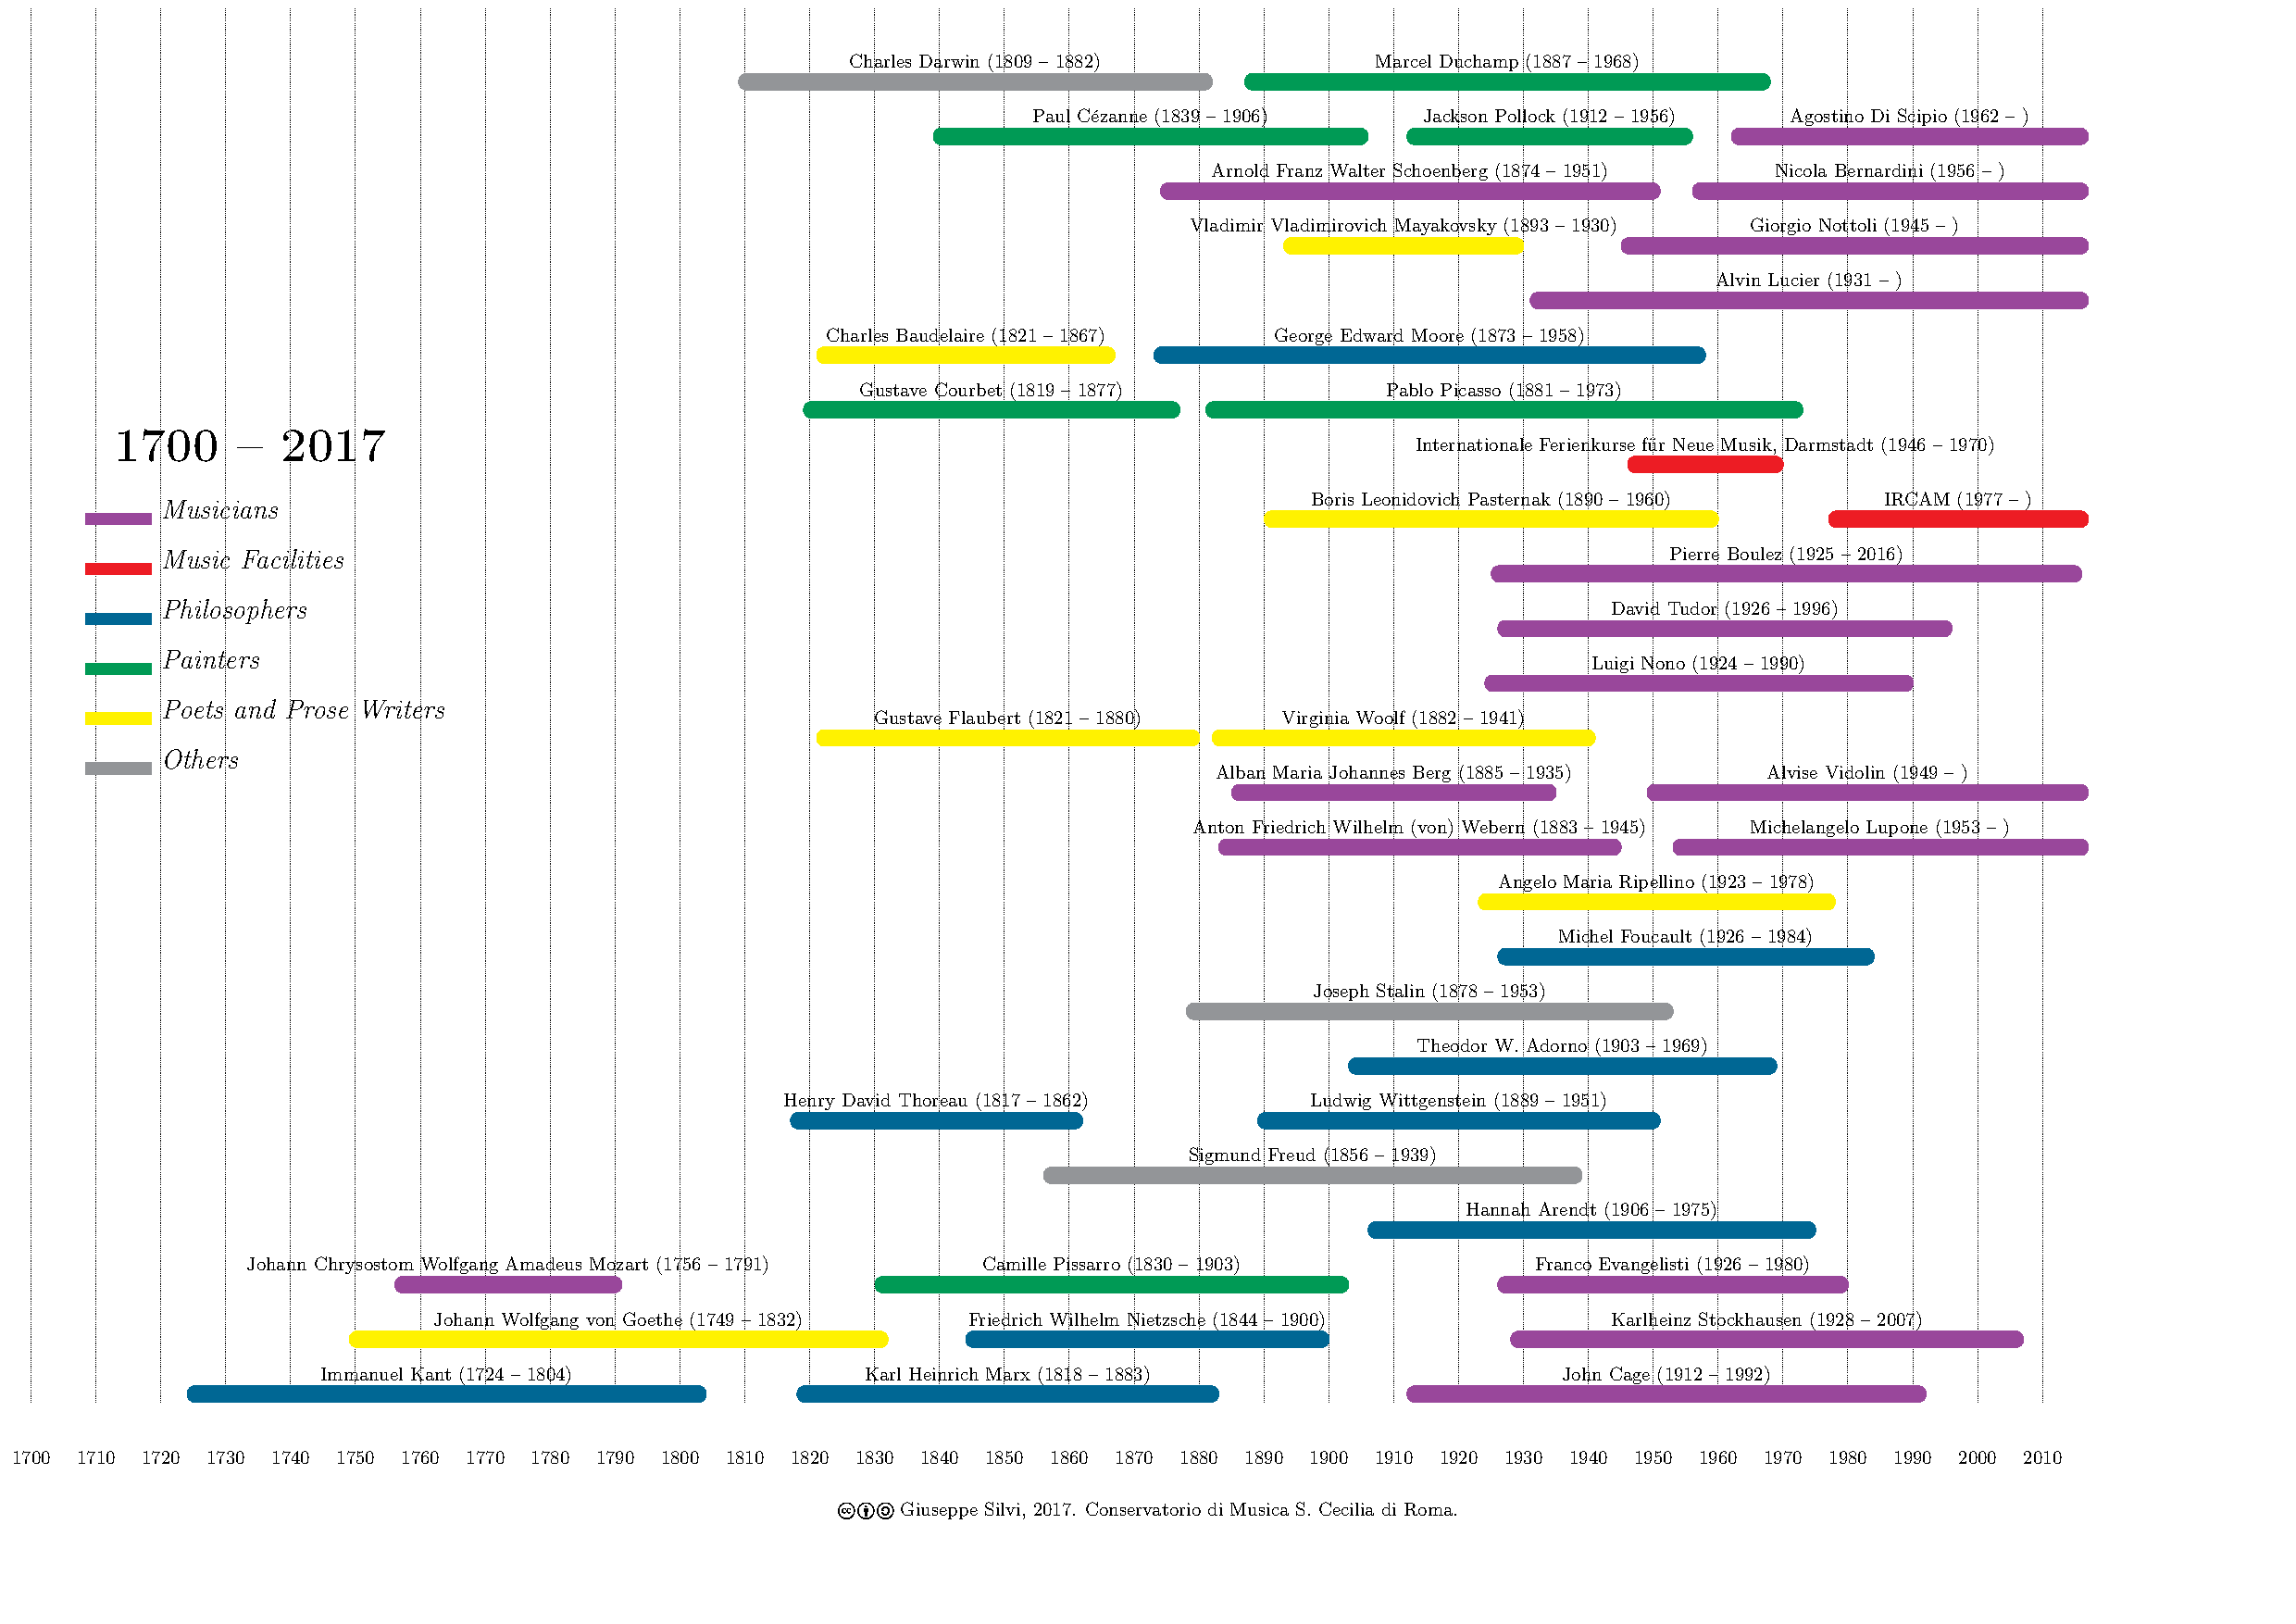
\includepdf[scale=2, offset= -250 0]{includes/_timeline/cosmologia.pdf}
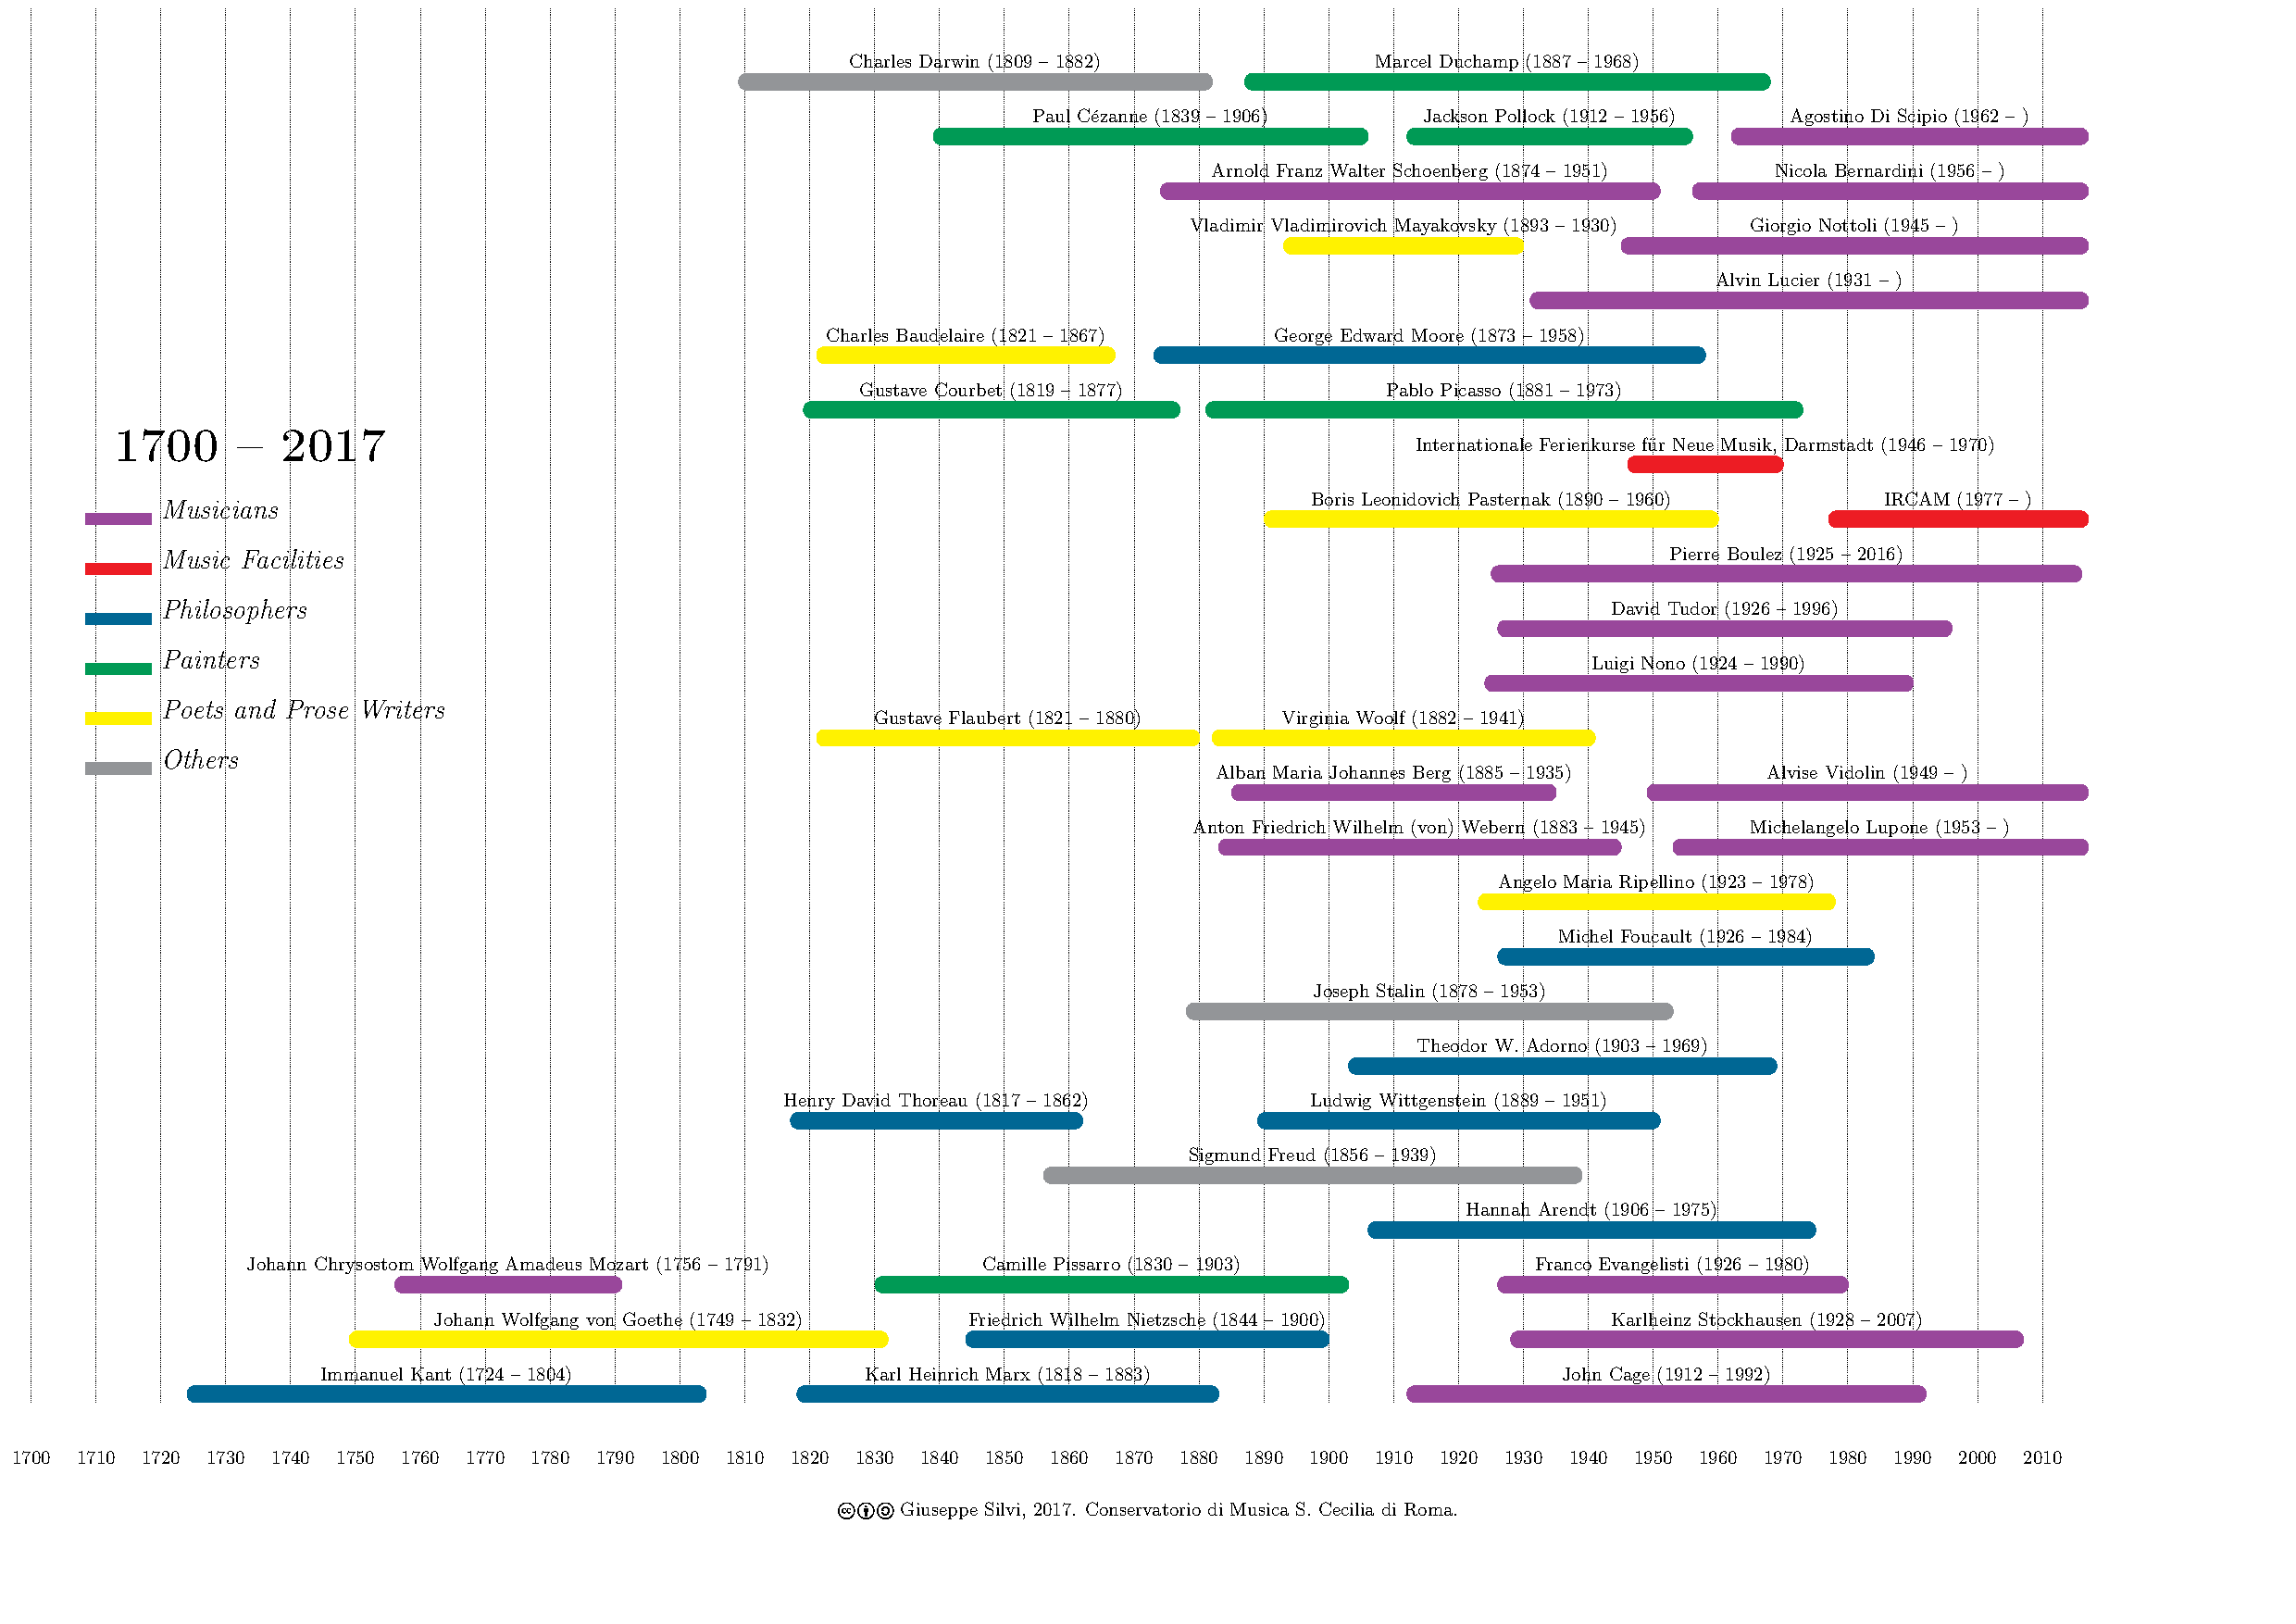
\includepdf[scale=2, offset= -210 0]{includes/_timeline/cosmologia.pdf}

\clearpage

\printindex

\clearpage

\printbibliography

\end{document}
